\documentclass[../MathsNotesBase.tex]{subfiles}




\date{\vspace{-6ex}}


\begin{document}
\searchableChapter{Analysis}{analysis}\clearpage

	\searchableSection{Real Analysis}{analysis}
	
	\searchableSubsection{Sets of Real Numbers}{analysis}{\bigskip		
		\subsubsection{Supremum and Infimum}
		\boxeddefinition{\textbf{(Bounded Set)} An \textit{upper bound} on a set A is a value $x$ such that,
			\[ \forall a \in A, \, a \leq x \]
			and a \textit{lower bound} is similarly defined as a value $y$ such that,
			\[ \forall a \in A, \, a \geq y. \]
			A set is said to be \textit{upper-bounded} if there exists some upper-bound on the set and is said to be \textit{lower-bounded} if there exists some lower bound on the set. If there exists both upper and lower bounds then the set is said to be \textit{bounded}.
		}
		
		\boxedaxiom{\textbf{(Continuum Property)} Every non-empty set of real numbers that is bounded above has a least upper bound and every non-empty set of real numbers that is bounded below has a greatest upper bound.}\label{axiom:continuum-property}
		
		\boxeddefinition{\textbf{(Supremum)} The \textit{supremum} of an upper-bounded set $A$ is a value $\sigma_A$ such that $\sigma_A$ is an upper bound on $A$ and, 
			\[ \sigma_A' < \sigma_A \iff \exists a \in A \suchthat a > \sigma_A' \]
			which is to say that if $\sigma_A' < \sigma_A$ then $\sigma_A'$ is not an upper bound on $A$ and, if $\sigma_A'$ is not an upper bound on $A$ then it must be less than $\sigma_A$ since $\sigma_A$ is an upper bound on A.\\
			
			An alternative, equivalent definition is: For $\sigma_A$, an upper bound on $A$,
			\[ \forall \epsilon > 0, \, \exists a \in A \suchthat a > \sigma_A - \epsilon. \]
		}\label{def:supremum}

		\note{Rearranging the alternative definition we obtain,
		\begin{align*}
			&&  \forall \epsilon > 0 \logicsep \exists a \in A &\suchthat a + \epsilon > \sigma_A  \\
			&\iff &\forall \epsilon > 0 \logicsep \exists a \in A &\suchthat \epsilon > \sigma_A - a  &\sidecomment{}
		\end{align*}
		which shows us that for any positive epsilon there needs to be an $a$ close enough to the value of $\sigma_A$ that the difference in their values is less than epsilon. Since $a$ can approach arbitrarily close to $\sigma_A$ this is achievable for any positive epsilon. This property seems to be equivalent to the fact that $\sigma_A$ is a \textit{limit point} of $A$ (see: Topology).}
		
		\boxeddefinition{The \textbf{infimum} of a lower-bounded set $A$ is defined similarly to the supremum: as a value $\tau_A$ such that $\tau_A$ is a lower bound on $A$ and, 
			\[ \tau_A' > \tau_A \iff \exists a \in A \suchthat a < \tau_A' \]
			or alternatively,
			\[ \forall \epsilon > 0, \, \exists a \in A \suchthat a < \tau_A + \epsilon. \]
		}\label{def:infimum}
		\notation{The supremum of $A$ is denoted ${ \sup A }$ and the infimum is denoted ${ \inf A }$.}
		
		
		
		\biggerskip		
		\labeledProposition{If a bounded set $A \subset \R{}$ has the property that,
			\[ \forall x,y \in A \logicsep \abs{x - y} < 1 \]
			then it follows that,
			\[ (\sup A - \inf A) \leq 1. \]
		}{sup_minus_inf_max_difference}
		\begin{proof}\nl[8]
			Let ${ \sigma_A = \sup A }$ and ${ \tau_A = \inf A }$. Then,
			\[ 
			\forall \epsilon_1 > 0 \logicsep \exists x \in A \suchthat x - \epsilon_1 < \tau_A \eqand 
			\forall \epsilon_2 > 0 \logicsep \exists y \in A \suchthat y + \epsilon_2 > \sigma_A. 
			\]
			If we let
			\[ 0 < \epsilon < \min \left\{ \epsilon_1, \epsilon_2 \right\} \]
			then ${ \forall \epsilon_1,\epsilon_2 > 0 \logicsep \exists x,y \in A }$ such that
			\[  (x - \epsilon < \tau_A) \; \land (y + \epsilon > \sigma_A) \]
			and so
			\begin{equation}
				\sigma_A - \tau_A < (y + \epsilon) - (x - \epsilon) = (y - x) + 2\epsilon. \tag{*}
			\end{equation}
			
			\nl[8]
			If we then, further constrict the value of $\epsilon$ so that
			\[ 0 < \epsilon < \min \left\{ \epsilon_1, \epsilon_2, \frac{\sigma_A - \tau_A}{2} \right\} \]
			then equation (*) becomes			
			\[ \sigma_A - \tau_A < (y - x) + 2\epsilon < (y - x) + (\sigma_A - \tau_A) \]
			so that ${ y - x > 0 }$.
			
			\nl[8]
			Now suppose, for contradiction, that ${ (\sigma_A - \tau_A) > 1 }$. Then we can say that,
			\[ \exists r > 0 \logicsep (\sigma_A - \tau_A) = 1 + r. \] 
			If we then, once again, further constrict $\epsilon$ such that,
			\[ 0 < \epsilon < \min \left\{ \epsilon_1, \epsilon_2, \frac{\sigma_A - \tau_A}{2}, \frac{r}{2} \right\} \]
			then equation (*) further becomes,
			\[\begin{aligned}
				&& \sigma_A - \tau_A &< (y - x) + 2\epsilon \\
				&\iff & \sigma_A - \tau_A &< (y - x) + r &\sidecomment{} \\
				&\iff & 1 + r &< (y - x) + r &\sidecomment{} \\
				&\iff & 1 &< y - x. 
			\end{aligned}\]
			
			Since ${ y - x > 0 }$ we, therefore, have
			\[ \abs{y - x} > 1 \]
			which contradicts the set property that $ \forall x,y \in A, \, \abs{x - y} < 1 $. So this shows that $ (\sigma_A - \tau_A) \leq 1 $.
		\end{proof}
		
		
		\bigskip
		\labeledProposition{Let $A \subset \R{}$ be a bounded set and let $B$ be the set defined by
			\[ B = \setc{b}{b = f(a), \; a \in A} \]
			where the function $f$ is some strictly monotonic function.
			Then it follows that,
			\[ \sup B = f(\sup A). \]
		}{monotonic_functions_preserve_supremum}
		\begin{proof}
			A is bounded and so ${ \sigma_A = \sup A }$ exists. So, using the supremum properties we have,
			\begin{align*}
				&& \forall a \in A \logicsep a &\leq \sigma_A  \\
				&\iff & \forall a \in A \logicsep f(a)  &\leq f(\sigma_A)  &\sidecomment{by monotonicity of f}\\
				&\iff & \forall b \in B \logicsep b  &\leq f(\sigma_A) 
			\end{align*}
			which is to say that $\sigma_B = f(\sigma_A)$ is an upper bound on $B$.\\
			Furthermore, using the other supremum property, we have that,
			\begin{align*}
				&& \sigma_A' < \sigma_A &\implies \exists a \in A \suchthat a > \sigma_A' \\
				&\iff & f(\sigma_A') < f(\sigma_A)  &\implies \exists a \in A \suchthat f(a) > f(\sigma_A')  &\sidecomment{by strict monotonicity of f}\\
				&\iff & \sigma_B' < \sigma_B  &\implies \exists b \in B \suchthat b > \sigma_B'.	
			\end{align*}
			Therefore $\sigma_B$ satisfies both requirements of the supremum and we have shown that,
			\[ \sup B = f(\sup A). \]
		\end{proof}



	
		
% -------------- break ----------------
\pagebreak



		\subsubsection{Open and Closed Sets in \texorpdfstring{$\R{}$}{R}}
		\note{\question{This material depends on sequence convergence covered later. Is it possible to fix this ordering?}}
		\bigskip
		\boxeddefinition{\textbf{(Neighbourhood)} The interval $ (L - \epsilon, L + \epsilon) $ is called the \textit{\mbox{$\epsilon$-neighbourhood of $L$}}.}
		
		\boxeddefinition{\textbf{(Open Sets in $\R{}$)} A set ${ X \subseteq \R{} }$ is an \textit{open set} iff every ${ x \in X }$ has an $\epsilon$-neighbourhood around it that is wholly contained in the set. That's to say,
			\[ \exists \epsilon > 0 \logicsep (x - \epsilon, x + \epsilon) \subseteq X. \]
		\label{def:open-set}}
	
		\boxeddefinition{\textbf{(Closed Set)} A set is a \textit{closed set} iff every convergent sequence of values in the set converges to a value contained in the set.\\
			
		Formally, if a set ${ X \subseteq \R{} }$ is a \textit{closed set} then every convergent sequence $(x_n)$ with ${ x_n \in X }$ for all ${ n \in \N{} }$ has
		\[ \lim_{n \to \infty} x_n \; \in X. \]
		\label{def:closed-set}}
		
		\note{Note that sets may be both open and closed or neither open or closed. For example:
			\begin{itemize}
				\item The set of all real numbers $\R{}$ is both open and closed; and
				\item the interval ${ (0,1] }$ is neither open nor closed.
			\end{itemize}
			It's also worth noting that ${ [1, \infty) }$ may appear to be neither open nor closed but is, in fact, closed.
		}
	
	
		\nl[12]
		\labeledProposition{The union of a collection of open sets is an open set.}{union-of-open-sets-is-an-open-set}
		\begin{proof}
			Let $I$ be some indexing set and ${ \setc{U_i}{i \in I} }$ be an indexed collection of sets. Then, if each $U_i$ is an open set, then we have, by the definition of an open set (\ref{def:open-set}), for all ${ i \in I }$,
			\[ \forall x \in U_i \logicsep \exists \epsilon > 0 \logicsep (x - \epsilon, x + \epsilon) \subseteq U_i. \]
			But also
			\[ (x - \epsilon, x + \epsilon) \subseteq U_i \; \implies \; (x - \epsilon, x + \epsilon) \subseteq \bigcup_{i \in I} U_i. \]
			Therefore, if each $U_i$ is an open set it follows that $\bigcup_{i \in I} U_i$ is an open set also.
		\end{proof}
	
		\bigskip
		\labeledProposition{The intersection of a collection of finitely many open sets is an open set.}{intersection-of-finitely-many-open-sets-is-an-open-set}
		\begin{proof}
			Let ${ I = \N{}_n = \{ 1, 2, \dots, n \} }$ and let every set in the indexed family ${ \setc{A_i}{i \in I} }$ be an open set. Then, if ${ x \in \bigcap_{i \in I} A_i }$ it follows that, for each ${ i \in I }$,
			\[ x \in A_i \; \implies \; \exists \epsilon_i \logicsep (x - \epsilon_i, x + \epsilon_i) \subseteq A_i. \]
			Since there are a finite number, $n$, of sets $A_i$ and so the set ${ \setc{\epsilon_i}{i \in I} }$ is also finite, then it has a minimum. If we take
			\[ \epsilon = \min \setc{\epsilon_i}{i \in I} \]
			then we have,
			\[ \forall i \in I \logicsep (x - \epsilon, x + \epsilon) \subseteq A_i \; \implies \; (x - \epsilon, x + \epsilon) \subseteq \bigcap_{i \in I} A_i.  \qedhere \]
		\end{proof}
	
		\bigskip
		\labeledProposition{The intersection of a collection of infinitely many open sets is not, in general, an open set.}{intersection-of-infinitely-many-open-sets-is-not-necessarily-an-open-set}
		\begin{proof}
			Let ${ \setc{U_i}{i \in \N{}} }$ be a family of open sets such that ${ U_i = (-1/i, 1/i) }$. Then, for ${ x \in \bigcap_{i \in I} U_i }$ it follows that, for each ${ i \in I }$,
			\[ x \in U_i \; \implies \; \exists \epsilon_i \logicsep (x - \epsilon_i, x + \epsilon_i) \subseteq U_i. \]
			However, in this case, if we take the minimum of the $\epsilon_i$, there is no minimum and instead we have an infimum,
			\[ \inf \setc{\epsilon_i}{i \in I} = \inf \setc{1/i}{i \in \N{}} = 0. \]
			Therefore, the widest neighbourhood that is contained in all the $U_i$ is ${ (x - 0, x + 0) }$ which is to say, no neighbourhood. So there is only a single element in ${ x \in \bigcap_{i \in I} U_i }$ and the only element that it can be is 0.
		\end{proof}
	
		
		\bigskip
		\labeledProposition{A set ${ C \subset \R{} }$ is closed iff its complement ${ \R{}\setminus C }$ is open.}{subset-of-R-is-closed-iff-complement-is-open}
		\begin{proof}
			Assume $C$ is closed. Then, by the definition of a closed set (\ref{def:closed-set}), for every sequence $(x_n)$,
			\[ \forall n \in \N{} \logicsep x_n \in C \; \implies \; \lim_{n \to \infty} x_n \; \in C. \]
			Suppose, for contradiction, that ${ \R{} \setminus C }$ is not open so that, negating the definition of an open set (\ref{def:open-set}), there exists some ${ x \in \R{} \setminus C }$ such that,
			\[ \forall \epsilon > 0 \logicsep (x - \epsilon, x + \epsilon) \centernot\subseteq \R{} \setminus C. \]
			But then, there exists some sequence $(x_n)$ with ${ \abs{x_n - x} = 1/n = \epsilon }$ such that
			\[ \forall n \in \N{} \logicsep x_n \in C \; \land \; \lim_{n \to \infty} x_n = x \; \centernot\in C. \]
			This contradicts the hypothesis that $C$ is a closed set and so ${ \R{} \setminus C }$ is open.\\
			
			\nl
			Conversely, suppose ${ \R{} \setminus C }$ is open and suppose, for contradiction, that $C$ is not closed. Then there exists some sequence $(x_n)$, such that
			\[ \forall n \in \N{} \logicsep x_n \in C \; \land \; \lim_{n \to \infty} x_n \; \centernot\in C. \]
			But then there is some ${ y = \lim_{n \to \infty} x_n \in \R{} \setminus C }$ with, for every ${ \epsilon > 0 }$, some $x_n$ such that
			\[ \abs{x_n - y} < \epsilon \; \implies \; x_n \in (y - \epsilon, y + \epsilon) \]
			which, since ${ x_n \in C }$, implies that
			\[ (y - \epsilon, y + \epsilon) \centernot\subseteq \R{} \setminus C \]
			contradicting the hypothesis that ${ \R{} \setminus C }$ is open. Therefore $C$ is closed.
		\end{proof}
	
		
		\nl[6]
		\sep
		\begin{exe}
			\ex Any open interval is an open set but the reverse is not, in general, the case. For example,
			\[ S = (1,2) \cup (3,4) \]
			is an open set but is not an open interval (it is not an interval at all).
			
			\bigskip
			\ex Let ${ I = (1,\infty) }$ be an indexing set and define the indexed collection of sets,
			\[ C = \setc{A_i}{i \in I} \suchthat A_i = (1/i, 2]. \]
			Then,
			\[ \bigcup_{i \in I} A_i = (0, 2]. \]
			
			\nl[12]
			For any ${ A_i \in C }$ we have ${ A_i \subseteq (0, 2] }$ and
			\[ \forall i \in I \logicsep A_i \subseteq (0, 2] \; \implies \; \bigcup_{i \in I} A_i \subseteq (0, 2]. \]
			Conversely, if ${ x \in (0, 2] }$ then ${ 0 < x \leq 2 }$. Since ${ I = (1,\infty) }$, for any ${ x \in (0, 2] }$, there exists ${ i \in I }$ such that
			\[ i > 1/x \; \implies \; 1/i < x \leq 2 \; \implies \; x \in A_i \; \implies \; x \in \bigcup_{i \in I} A_i. \]
			Therefore ${ (0, 2] \subseteq \bigcup_{i \in I} A_i }$.
		\end{exe}
	
	
		\nl[16]
		\subsubsubsection{Open and Closed Sets in \texorpdfstring{$\R{m}$}{Rm}}
		\nl[4]
		\boxeddefinition{\textbf{(Open Ball)} For ${ \x \in \R{m} }$ and ${ \epsilon > 0 \in \R{} }$, the \textit{open ball of radius $\epsilon$ around $\x$} is defined as the set,
		\[ B_{\epsilon}(\x) = \setc{\y}{ \norm{\x - \y} < \epsilon }. \]
		\label{def:open-ball}}
	
		\boxeddefinition{\textbf{(Open Set in $\R{m}$)} A set ${ X \subseteq \R{m} }$ is \textit{open} iff, for any ${ \x \in X }$, there exists ${ \epsilon > 0 }$ such that,
			\[ B_{\epsilon}(\x) \subseteq X. \]
		\label{def:open-set-in-Rm}}
	
		\biggerskip
		\labeledProposition{Any open ball is an open set.}{open-ball-is-open-set}
		\begin{proof}
			Let ${ B_\epsilon(\x) }$ be an open ball around an element ${ \x \in X \subseteq \R{m} }$. Then for any ${ \y \in B_\epsilon(\x) }$ there exists
			\[ \delta = \epsilon - \norm{\x - \y} > 0 \]
			such that, for any ${ \z \in B_\delta(\y) }$,
			\[ \norm{\x - \z} = \norm{\x - \y + \y - \z} \leq \norm{\x - \y} + \norm{\y - \z} < \norm{\x - \y} + \delta = \epsilon. \]
			Therefore ${ \z \in B_\epsilon(\x) }$ and so
			\[ B_\delta(\y) \subseteq B_\epsilon(\x). \]
			So ${ B_\epsilon(\x) }$ is an open set.
		\end{proof}
	
		\bigskip
		\labeledProposition{Theorem 5.7}{}
		\begin{proof}
			\nl[6]\TODO{complete this}
		\end{proof}
	
	
		\biggerskip
		\subsubsection{Compactness}
		\bigskip
		\boxeddefinition{\textbf{(Compact Set)} A set ${ C \subseteq \R{m} }$ is \textit{compact} iff, any sequence with all its terms in $C$, has a convergent subsequence converging to a point in $C$.
		\label{def:compact-set}}
	
		\biggerskip
		\labeledTheorem{\textbf{(Heine-Borel Theorem)} A set ${ C \subseteq \R{m} }$ is \textit{compact} iff it is both closed and bounded.}{heine-borel}
		\begin{proof}
			\nl[6]\TODO{complete this}
		\end{proof}
	
		\labeledTheorem{Theorem 5.11}{}
		\begin{proof}
			\nl[6]\TODO{complete this}
		\end{proof}
	}



	
% --------------- break ---------------	
\pagebreak


	\searchableSubsection{Sequences}{analysis}{
	
		\biggerskip
		\boxeddefinition{\textbf{(Sequence)} A (real-valued) \textit{sequence} is a function from the naturals to the reals,
			\[ f: \N{}\longmapsto \R{}. \]
			The value $f(n)$ is called the \textit{n\textsuperscript{th} term} of the sequence.\\
			
			A sequence may be defined either:
			\begin{itemize}
				\item{Explicitly, by defining the function $f$ as an expression of the term number $n$,
					\[ f(n) = h(n) \]
					where $h$ is some real-valued function of arity 1.
				}
				\item{Inductively, by specifying one or more initial terms and a recurrence that specifies term $n$ as a function of one or more previous terms,
					\[\begin{aligned}
						&f(1) = \alpha_1, \, \dots , \, f(k) = \alpha_k, \nn
						&f(n) = h(f(n-1), \dots, f(n-k))
					\end{aligned}\]
					where ${ \alpha_1, \dots, \alpha_k \in \R{} }$ and $h$ is some real-valued function of arity $k$.
				}
			\end{itemize}
		}
		\notation{A sequence may be denoted $(f(n))_{n=1}^\infty$ or $(f(n))$, where $f$ is the function that defines the sequence or, a more informal notation is common where $(a_n)_{n=1}^\infty$ or $(a_n)$ (or sometimes $\{a_n\}$) is used to denote the sequence with $a_n$ referring to the $n$-th term.
		}
		
		\bigskip
		\boxeddefinition{\textbf{(Bounded Sequence)} If $a_n$ is a sequence and $ S = \setc{a_n}{n \in \N{}} $ then $a_n$ is said to be \textbf{bounded below} if $S$ has a lower bound and \textbf{bounded above} if $S$ has an upper bound, and \textbf{bounded} if it is bounded above and below.
		}\label{def:bounded-sequence}
		
		\boxeddefinition{An \textbf{increasing} sequence is a sequence $a_n$ such that,
			\[ \forall n \in \N{} \logicsep a_{n+1} \geq a_n \]
			and \textbf{decreasing} if,
			\[ \forall n \in \N{} \logicsep a_{n+1} \leq a_n \]
			and \textbf{monotonic} if either increasing or decreasing.
		}
	
		\subsubsection{Limits of Sequences}
		\bigskip
		\boxeddefinition{\textbf{(Sequence Convergence)} A sequence $a_n$ is said to \textit{tend} to $L$ or have the \textit{limit} $L$ iff,
			\[ \forall \epsilon > 0 \in \R{} ,\, \exists N \in \N{} \suchthat \forall n > N ,\, \abs{a_{n} - L} < \epsilon. \]
			In such a case, the sequence is said to be \textit{convergent}.
		}\label{def:seq-tends-to-L}
		
		\boxeddefinition{\textbf{(Sequence Divergence)} A sequence $a_n$ is said to \textit{tend to infinity} iff,
			\[ \forall M > 0 \in \R{} ,\, \exists N \in \N{} \suchthat \forall n > N ,\, a_{n} > M \]
			and \textit{tend to minus-infinity} iff,
			\[ \forall M < 0 \in \R{} ,\, \exists N \in \N{} \suchthat \forall n > N ,\, a_{n} < M. \]
			In either case, or if the sequence oscillates without converging, the sequence is described as \textit{divergent}.
		}\label{def:seq-diverges}
		
		\note{A mnemonic for the taxonomy of convergence/divergence behaviours.\\\\
			\begin{tabular}[h!]{|c|c|c|c|}
				\cline{1-4}
				convergent & \multicolumn{3}{c|}{divergent}\\
				\cline{1-4}
				bounded & bounded & \multicolumn{2}{c|}{unbounded} \\
				\cline{2-4}
				& oscillatory & oscillatory & non-oscillatory \\
				\cline{3-4}
				& & unbounded oscillatory & ${ \to \infty }$ or ${ \to -\infty }$\\
				\cline{1-4}
			\end{tabular}
		}		
		
		\bigskip
		\note{Note that if we were to use a less formal description of a limit, for example, if we say that a sequence tends to some value $L$ when the terms of the sequence \textit{get closer and closer to} $L$, then we encounter the following problems:
			\begin{itemize}
				\item{that the sequence gets closer and closer to many numbers so that this does not specify a single specific limit.}
				\item{that the sequence can have a limit but it's not the case that every term is closer than the previous term to the limit. For example,
					\[ a_{2k} = 1/k, \; a_{2k - 1} = \frac{1}{k+1} \]
					tends to 0 but $ a_{2k} > a_{2k - 1} $.
				}
			\end{itemize}
		}
	
		
		
			
		\bigskip	
		\labeledProposition{A sequence has at most one limit. In other words, a sequence can only converge, if at all, to a single unique value.}{uniqueness_of_limits}
		\begin{proof}
			Suppose $L_1$ and $L_2$ are both limits of the sequence $a_n$ and that
			\[  L_1 \neq L_2 \implies \abs{L_2 - L_1} = d > 0. \]
			By the definition of the limit of a sequence \ref{def:seq-tends-to-L},
			\[ \forall \epsilon_1 > 0 \in \R{} \logicsep \exists N_1 \in \N{} \logicsep \forall n > N_1 \logicsep \abs{a_n - L_1} < \epsilon_1, \]
			\[ \forall \epsilon_2 > 0 \in \R{} \logicsep \exists N_2 \in \N{} \logicsep \forall n > N_2 \logicsep \abs{a_n - L_2} < \epsilon_2. \]
			Let ${ \epsilon_1 = \epsilon_2 = \epsilon }$ so that, for all $\epsilon$,
			\[ \exists N = \max \{ N_1, N_2 \} \logicsep \forall n > N \logicsep \abs{a_n - L_1} < \epsilon \; \land \; \abs{a_n - L_2} < \epsilon. \]
			Then,
			\[ \abs{L_2 - L_1} = \abs{(L_2 - a_n) + (a_n - L_1)} \leq \abs{L_2 - a_n} + \abs{L_1 - a_n} < 2\epsilon. \]	
			So, if we restrict the value of $\epsilon$ so that
			\[ 0 < \epsilon < \frac{d}{2} \]
			then
			\[ \abs{L_2 - L_1} < 2\epsilon < d. \]
			But this is a contradiction of the hypothesis that ${ \abs{L_2 - L_1} = d }$ and we can therefore deduce that ${ L_1 = L_2 }$.
		\end{proof}	
		
		\bigskip
		\begin{lemma}
			Any finite set of elements from an ordered field has a minimum and a maximum.
		\end{lemma}
		\begin{proof}
			This can be proven quite easily using induction. Taking the base case of a set of cardinality one, clearly there is a maximum and a minimum both of which are the sole element of the set. Then, the induction step is to say, given a set $S$ that has a maximum, $s_{max}$, and a minimum, $s_{min}$, if we add a new element $e$, then if $e$ is greater than $s_{max}$ it is the maximum of the new set and if it is less than $s_{min}$ it is the minimum of the new set. Otherwise, the previous maximum and minimum also pertain to the new set. Therefore, adding a new element to a set that has a maximum and a minimum creates a new set with a maximum and a minimum.
			\note{This is in fact the \textit{Well-Ordering Principle} (see: \ref{sssection:well-ordering-theorem}).}
		\end{proof}
	
		\bigskip
		\labeledProposition{Any convergent sequence is bounded.}{convergent_seqs_bounded}
		\begin{proof}
			Let $a_n$ be an arbitrary convergent sequence so that,
			\[ \forall \epsilon > 0 \in \R{} \logicsep \exists N \in \N{} \logicsep \forall n > N \logicsep \abs{a_n - L} < \epsilon. \]
			Now choose some value of $\epsilon$ and then there exists some ${ N \in \N{} }$ such that ${ \forall n > N }$,
			\[\begin{aligned}
				&& \abs{a_n - L} &< \epsilon \\
				&\iff & -\epsilon < a_n - L &< \epsilon  &\sidecomment{} \\
				&\iff & L - \epsilon < a_n &< L + \epsilon.
			\end{aligned}\]
			That's to say, the sequence for values of ${ n > N }$ is bound within the $\epsilon$-neighbourhood of $L$.\\
			
			Meanwhile the sequence for values of ${ n \leq N }$ is a finite set of values in $\R{}$, an ordered field. So, by the \textit{Well-Ordering Principle} (see: \ref{sssection:well-ordering-theorem}), it has a minimum and a maximum, which we denote $m_1$ and $M_1$ respectively,
				\[ m_2 = \min \setc{a_n}{n \leq N}  \eqand  M_1 = \max \setc{a_n}{n \leq N}. \]
			On the other hand, for the values of the sequence for ${ n > N }$,
				\[ m_2 = \min \setc{a_n}{n > N} = L - \epsilon \eqand M_2 = \max \setc{a_n}{n > N} = L + \epsilon. \]
			So clearly then, all values in the whole sequence are bounded below by the minimum of these two minima,
				\[ S_{min} = \min \setc{a_n}{n \in N} = \min \{m_1, m_2\}, \]
			and above by the maximum of these maxima,
				\[ S_{max} = \max \setc{a_n}{n \in N} = \max \{M_1, M_2\}. \]
			Therefore, the sequence $a_n$ is bounded.
		\end{proof}
		
		
		\bigskip
		\labeledProposition{Any increasing sequence that is bounded above has a limit.}{increasing_bounded_seqs_have_limit}
		\begin{proof}
			Let $a_n$ be an increasing sequence that is bounded above. Then,
			\[ \forall n \in \N{} \logicsep a_{n+1} \geq a_n \]
			and let ${ S = \setc{a_n}{n \in \N{}} }$. Since $a_n$ is bounded above, by the Continuum Property (\autoref{axiom:continuum-property}) it has a supremum. Let $ \sigma = \sup S $ be the supremum so that,
			\[ \forall a_n \in S \logicsep a_n \leq \sigma \eqand \forall \epsilon > 0 \in \R{} \logicsep \exists a_n \in S \logicsep a_n > \sigma - \epsilon. \]
			So if we choose any fixed value of $\epsilon$ then there exists some ${ a_n \in S }$ such that
			\[ a_n > \sigma - \epsilon \iff a_n - \sigma > -\epsilon \iff \sigma - a_n < \epsilon. \]
			Furthermore, since $\sigma$ is an upper bound on the values $a_n$, the expression ${ \sigma - a_n }$ is positive and so this last result implies
			\[ \sigma - a_n = \abs{a_n - \sigma} < \epsilon. \]
			Since the sequence is increasing and ${ a_{n+1} \geq a_n }$,
			\[ -a_{n+1} \leq -a_n \iff \sigma - a_{n+1} \leq \sigma - a_n < \epsilon \implies \sigma - a_{n+1} < \epsilon. \]
			Again, because $\sigma$ is an upper bound on the values of the sequence we have,
			\[  \sigma - a_{n+1} = \abs{a_{n+1} - \sigma} < \epsilon. \]
			Therefore, we have shown that,
			\[ \abs{a_n - \sigma} < \epsilon \implies \abs{a_{n+1} - \sigma} < \epsilon \]
			and so we can reason inductively that, if we let ${ N = n }$, then
			\[ \forall n > N \logicsep \abs{a_n - \sigma} < \epsilon. \]
			This result was shown for an arbitrary, strictly positive, value of $\epsilon$ so we therefore have,
			\[ \forall \epsilon > 0 \in \R{} \logicsep \exists N \in \N{} \logicsep \forall n > N \logicsep \abs{a_n - \sigma} < \epsilon \]
			which, by the definition of the limit of a sequence (\ref{def:seq-tends-to-L}), is to say that the sequence $a_n$ converges to the limit $\sigma$.
		\end{proof}
		
		\medskip
		\begin{corollary}\label{coro:increasing-seq-bounded-above-converges-to-supremum}
			Any increasing sequence that is bounded above converges to the supremum of its elements (terms, values, etc.).
		\end{corollary}
		\begin{corollary}\label{coro:decreasing-seq-bounded-below-converges-to-infimum}
			A decreasing sequence that is bounded below converges to the infimum of its elements.
		\end{corollary}
	
		\bigskip
		\labeledProposition{If a sequence $a_n$ converges to $L$ and ${ a_n \geq M }$ for all ${ n \in \N{} }$ then,
			\[ L \geq M. \]
		}{if-a-seq-is-geq-M-and-converges-to-L-then-L-is-geq-M}
		\begin{proof}
			By the definition of the limit of a sequence (\ref{def:seq-tends-to-L}),
			\[ \forall \epsilon > 0 \in \R{} \logicsep \exists N \logicsep \forall n > N \in \N{} \logicsep \abs{a_n - L} < \epsilon. \]
			Suppose, for contradiction, that ${ L < M }$. Then there exists ${ \epsilon = M - L > 0 \in \R{} }$ and since ${ a_n \geq M }$, we have for all $n$,
			\[ a_n \geq M \iff a_n - L \geq M - L = \epsilon. \]
			But the definition of the limit of $a_n$ implies that
			\[ -\epsilon < a_n - L < \epsilon \]
			and so, ${ L < M }$ and ${ a_n \geq M }$ together, contradict the convergence of $a_n$ to $L$.\\
			It follows that ${ L \geq M }$.
		\end{proof}
	
		\bigskip
		\labeledProposition{If a sequence $(a_n)$ converges to $L$ and a sequence $(b_n)$ converges to $M$ then,
			\[ \forall n \in \N{} \logicsep a_n \leq b_n \implies L \leq M. \]
		}{seq-terms-geq-implies-seq-limit-geq}
		\begin{proof}
			Assume for contradiction that ${ L > M }$. Then there exists some ${ \epsilon = \frac{L - M}{4} > 0 \in \R{} }$ so that,
			\[ \exists N_1 \logicsep \forall n > N_1 \in \N{} \logicsep \abs{a_n - L} < \epsilon = \frac{L - M}{4} \]
			and also
			\[ \exists N_2 \logicsep \forall n > N_2 \in \N{} \logicsep \abs{b_n - M} < \epsilon = \frac{L - M}{4} \]
			so we can take ${ N = \max \{N_1,N_2\} }$ and then, for all ${ n > N \in \N{} }$,
			\[ \abs{(a_n - b_n) + (M - L)} = \abs{(a_n - L) + (M - b_n)} \leq \abs{a_n - L} + \abs{b_n - M} < 2\epsilon. \]
			It follows then that,
			\[\begin{aligned}
				&& \abs{(a_n - b_n) + (M - L)} &< \frac{L - M}{2} \nn
				&\iff & \frac{M - L}{2} < (a_n - b_n) + (M - L) &<  \frac{L - M}{2} &\sidecomment{} \nn
				&\iff & \frac{1}{2}(L - M) < a_n - b_n &<  \frac{3}{2}(L - M).
			\end{aligned}\]
			But the assumption ${ L > M }$ implies that ${ L - M > 0 }$ so the above result implies that ${ a_n - b_n > 0 }$ also. This contradicts the construction of the sequences in which ${ a_n \leq b_n }$ for all $n$.
		\end{proof}

	
		
	
		\nl[40]
		\labeledProposition{
			Let $a_n$ and $b_n$ be convergent sequences with limits $ a $ and $ b $,
			respectively. Let $ C $ be a real number and let $ k $ be a positive integer. Then as $n \to \infty$,
			\begin{enumerate}[label=\alph*)]
				\item{$ Ca_n \to Ca $}
				\item{$ \abs{a_n} \to \abs{a} $}
				\item{$ a_n + b_n \to a + b $}
				\item{$ a_nb_n \to ab $}
				\item{$ {a_n}^k \to a^k $}
				\item{if, for all $n,\, b_n \neq 0$ and $b \neq 0$, then $\frac{1}{b_n} \to \frac{1}{b}$}.
			\end{enumerate}
			\smallskip
		}{seq_limit_properties}	
		\begin{proof}
			We prove each property individually in the given order.
			
			\subheading{Proof of (a) $ Ca_n \to Ca $} 
			If $ C = 0 $ then $ Ca_n = 0 = Ca $ for all $n$ and the proposition holds trivially. If $ C \neq 0 $ then, since $a_n \to a$,
			\[ \forall \epsilon' > 0 \logicsep \exists N \logicsep \forall n > N \in \N{} \logicsep \abs{a_n - a} < \epsilon'. \]
			Now let $ \epsilon = \abs{C}\epsilon' $. Then,
			\begin{align*}
				&& \forall \epsilon' > 0 \logicsep \exists N \logicsep \forall n > N \in \N{} &\logicsep \abs{C}\abs{a_n - a} < \abs{C}\epsilon' = \epsilon  \\
				&\iff & \forall \epsilon > 0 \logicsep \exists N \logicsep \forall n > N \in \N{} &\logicsep \abs{Ca_n - Ca} < \epsilon. &\sidecomment{$\abs{x}\abs{y} = \abs{xy}$ \ref{prop:product-of-absolute-vals-is-absolute-val-of-product}} \\
			\end{align*}
			
			\subheading{Proof of (b) $ \abs{a_n} \to \abs{a} $} 
			\begin{align*}
				&& \abs{a_n} = \abs{a_n - a + a} &\leq \abs{a_n - a} + \abs{a}  &\sidecomment{by triangle inequality \ref{sssection:triangle-inequality}}\\
				&\iff & \abs{a_n} - \abs{a} &\leq \abs{a_n - a}. &\sidecomment{(1)} \\
			\end{align*}
			\begin{align*}
				&& \abs{a} = \abs{a - a_n + a_n} &\leq \abs{a - a_n} + \abs{a_n}  &\sidecomment{by triangle inequality \ref{sssection:triangle-inequality}}\\
				&\iff & \abs{a} - \abs{a_n} &\leq \abs{a - a_n} = \abs{a_n - a} &\sidecomment{} \\
				&\iff & \abs{a_n} - \abs{a} &\geq -\abs{a_n - a}. &\sidecomment{(2)} \\
			\end{align*}
			Putting (1) and (2) together we have,
			\begin{align*}
				&& -\abs{a_n - a} &\leq \abs{a_n} - \abs{a} \leq \abs{a_n - a} &\sidecomment{by triangle inequality \ref{sssection:triangle-inequality}}\\
				&\iff & \abs{\abs{a_n} - \abs{a}} &\leq \abs{a_n - a}. \\
			\end{align*}
			The fact that $a_n$ converges to $a$ implies that $ \abs{a_n - a} $ converges to zero. Since it is an upper bound on the value of ${ \abs{\abs{a_n} - \abs{a}} }$, the value ${ \abs{\abs{a_n} - \abs{a}} }$ must also converge to zero. Specifically any value of $ n, \epsilon $ such that ${ \abs{a_n - a} < \epsilon }$ will also satisfy ${ \abs{\abs{a_n} - \abs{a}} \leq \abs{a_n - a} < \epsilon }$.
			
			\subheading{Proof of (c) $ a_n + b_n \to a + b $}
			Using, again, the "triangle inequality" \ref{sssection:triangle-inequality},
			\[ \abs{(a_n + b_n) - (a + b)} = \abs{(a_n - a) + (b_n - b)} \leq \abs{a_n - a} + \abs{b_n - b}. \]
			So, ${ \abs{a_n - a} + \abs{b_n - b} }$ is an upper bound on the value of ${ \abs{(a_n + b_n) - (a + b)} }$. If we take any arbitrary ${ \epsilon > 0 }$ then,
			\[ \exists N_1 \logicsep \forall n > N_1 \in \N{} \logicsep \abs{a_n - a} < \frac{\epsilon}{2} \]
			and
			\[ \exists N_2 \logicsep \forall n > N_2 \in \N{} \logicsep \abs{b_n - b} < \frac{\epsilon}{2}. \]
			Then, if we take $ N = \max \{N_1, N_2\} $, we have,
			\[ \forall n > N \in \N{} \logicsep \abs{(a_n + b_n) - (a + b)} \leq \abs{a_n - a} + \abs{b_n - b} < \epsilon. \]
			
			\subheading{Proof of (d) $ a_nb_n \to ab $}
			Again using the triangle inequality \ref{sssection:triangle-inequality},
			\begin{align*}
				&& \abs{a_nb_n - ab} = \abs{a_nb_n - ab_n + ab_n - ab} &\leq \abs{b_n(a_n - a)} + \abs{a(b_n - b)}  &\sidecomment{}\\
				&\iff & \abs{a_nb_n - ab} &\leq \abs{b_n}\abs{a_n - a} + \abs{a}\abs{b_n - b}.
			\end{align*}
			Since $b_n$ converges, by \autoref{prop:convergent_seqs_bounded}, it is bounded. Therefore, $\abs{b_n}$ has some upper bound which we shall call $B_U$. Then, if we take some arbitrary value of ${ \epsilon > 0 }$,
			\[ \exists N_1  \in \N{} \logicsep \forall n > N_1 \logicsep \abs{a_n - a} < \frac{\epsilon}{2B_U} \]
			and
			\[ \exists N_2 \in \N{} \logicsep \forall n > N_2 \logicsep \abs{b_n - b} < \frac{\epsilon}{2\abs{a}}. \]
			Now if we let ${ N = \max \{N_1, N_2\} }$ then
			\[\begin{aligned}
				&& \forall n > N \logicsep B_U\abs{a_n - a} + \abs{a}\abs{b_n - b} &< \epsilon \\
				&\iff & \forall n > N \logicsep \abs{a_nb_n - ab} &< \epsilon.
			\end{aligned}\]
			
			
			\subheading{Proof of (e) $ {a_n}^k \to a^k $}
			Using (d) - and because $k$ is a positive integer - we can do induction on the power $k$.\\
			Base cases 0 and 1 are clearly true as ${ k = 0 }$ results in $a_n$ being the constant 1 for all $n$ and so trivially converges to ${ a = 1 }$; and ${ k = 1 }$ results in the same sequence as $a_n$.\\
			So, we perform the induction step for ${ k \geq 2 }$. Then, by the induction hypothesis, ${ {a_n}^{k-1} \to a^{k-1} }$. But ${ {a_n}^k = {a_n}^{k-1}a_n }$ and, by (d) and the induction hypothesis, we have that ${ {a_n}^{k-1}a_n \to a^{k-1}a = a^k }$. Therefore, ${ {a_n}^k \to a^k. }$
			
			\subheading{Proof of (f) $ \forall n \logicsep b_n, b \neq 0 \implies \frac{1}{b_n} \to \frac{1}{b} $}
			Again invoking \autoref{prop:convergent_seqs_bounded} and letting the lower bound on the sequence $b_n$ be $B_L$,
			\[ \abs{\frac{1}{b_n} - \frac{1}{b}} = \abs{\frac{b - b_n}{b_nb}} = \abs{\frac{b_n - b}{b_nb}} = \frac{ \abs{b_n - b} }{ \abs{b_n}\abs{b} } \leq \frac{1}{B_L\abs{b}}\abs{b_n - b}. \]
			Now, since $\frac{1}{B_L\abs{b}}$ is a constant we can define the constant ${ C = \frac{1}{B_L\abs{b}} }$ and then we see that in (a) we have already proven that ${ C\abs{b_n - b} }$ converges to 0. In (a) we used that to prove that ${ Cb_n \to Cb }$ but here it proves that ${ \frac{1}{b_n} \to \frac{1}{b}. }$
		\end{proof}
	
	
		
		
		
		\nl[20]
		\begin{lemma}\label{lem:one-plus-h-to-the-power-n-is-geq-one-plus-hn}
			For all ${ n \in \N{} }$ and any fixed ${ h > 0 \in \R{} }$,
			\[ (1 + h)^n \geq 1 + hn. \]
		\end{lemma}
		\begin{proof}
			Clearly the hypothesis holds for ${ n = 0 }$
			\[ (1 + h)^0 = 1 = 1 + 0, \]
			and for ${ n = 1 }$
			\[ (1 + h)^1 = 1 + h. \]
			Assume the hypothesis is correct for some ${ n-1 > 1 }$. Then,
			\[\begin{aligned}
				(1 + h)^n &= (1 + h)(1 + h)^{n-1} \\
				&\geq (1 + h)(1 + (n-1)h) &\sidecomment{by induction hypothesis} \\
				&= 1 + nh + (n-1)h^2 \\
				&> 1 + nh.  &\sidecomment{${ \because (n-1),h > 0 }$}
			\end{aligned}\]	
		\end{proof}
	
		\bigskip
		\labeledProposition{If $x_n$ is a sequence and $\abs{x_n}$ tends to infinity as ${ n \to \infty }$ then the sequence diverges.}{if-abs-value-of-seq-tends-to-infinity-seq-diverges}
		\begin{proof}
			Assume for contradiction that $x_n$ converges to some finite limit $L$. Then,
			\[ \forall \epsilon > 0 \in \R{} \logicsep \exists N_1 \logicsep \forall n > N_1 \logicsep \abs{x_n - L} < \epsilon. \]
			But, since $\abs{x_n}$ tends to infinity as ${ n \to \infty }$, we also have,
			\[ \forall M > 0 \in \R{} \logicsep \exists N_2 \logicsep \forall n > N_2 \abs{x_n} > M. \]
			Therefore, if we choose any such arbitrary value of $\epsilon$ and let ${ M = \epsilon + \abs{L} }$, then there exists some ${ N = \max \{N_1,N_2\} }$ such that, for all ${ n > N }$,
			\[ \abs{x_n} > M \implies \abs{x_n} > \epsilon + \abs{L} \]
			and also
			\[ \abs{x_n} = \abs{x_n - L + L} \leq \abs{x_n - L} + \abs{L} < \epsilon + \abs{L}. \]
			This is clearly a contradiction and so we conclude that $x_n$ does not converge to a finite limit.
		\end{proof}
	
		\bigskip
		\labeledProposition{If $x_n$ is a sequence and $\abs{x_n}$ tends to 0 as ${ n \to \infty }$ then the sequence converges to 0. That's to say,
			\[ \lim_{n \to \infty} \abs{x_n} = 0 \implies \lim_{n \to \infty} x_n = 0. \]
		}{abs-val-of-seq-tends-to-0-then-seq-tends-to-0}
		\begin{proof}
			This follows from the fact that ${ \abs{x_n} = \abs{\abs{x_n}} = \abs{\abs{x_n} - 0} }$ so that
			\[ \abs{x_n} < \epsilon \iff \abs{\abs{x_n} - 0} < \epsilon. \]
		\end{proof}
		\note{Note that this \textbf{only} applies when the limit is 0. If we had ${ \lim_{n \to \infty} \abs{x_n} = 1 }$ for instance, then it could be that the sequence was divergently oscillating between 1 and -1.}
	
		\bigskip
		\labeledProposition{A sequence of the form,
			\[ x_n = a x_{n-1} \]
			with initial value $x_0$, can only diverge or converge to 0 or $x_0$.
		}{geometric-progression-sequence-diverges-or-converges-to-0-or-initial-value}
		\begin{proof}
			Consider the sequence $\abs{x_n}$, 
			\[ \abs{x_n} = \abs{a^n x_0} = \abs{a^n} \abs{x_0} = \abs{a}^n \abs{x_0}. \]
			
			Now we divide the possible values of $\abs{a}$ into 3 cases:
			\begin{enumerate}[label=(\roman*)]
				\item{${ \abs{a} > 1 }$\\
					
					Observe that
					\[ \abs{a} > 1 \implies \exists h > 0 \in R{} \suchthat \abs{a} = 1 + h. \]
					By \autoref{lem:one-plus-h-to-the-power-n-is-geq-one-plus-hn}, for all ${ n \in \N{} }$,
					\[ \abs{a}^n = (1 + h)^n \geq 1 + hn. \]
					If we choose any arbitrarily large ${ M \in \R{} }$ then, because
					\[ 1 + hn > M \iff hn > M - 1 \iff n > \frac{M - 1}{h}, \]
					there exists
					\[ N = \frac{M - 1}{h} \in \R{} \]
					such that
					\[ \forall n > N \in \N{} \logicsep 1 + hn > M \implies \abs{a}^n > M. \]
					Therefore $\abs{a}^n$ tends to infinity and so also
					\[ \abs{a}^n \abs{x_0} = \abs{x_n} \]
					tends to infinity as ${ n \to \infty }$. So, by \autoref{prop:if-abs-value-of-seq-tends-to-infinity-seq-diverges}, we can conclude that $x_n$ diverges.
				}
				\bigskip
				\item{${ \abs{a} = 1 }$\\
					
					In this case, either:
					\begin{itemize}
						\item{${ a = 1 }$ and for all ${ n \in \N{} }$, ${ x_n = x_0 }$ so that the sequence converges to $x_0$; or else}
						\item{${ a = -1 }$ and the sequence alternates between 1 and -1 and so diverges.}
					\end{itemize} 
				}
				\bigskip
				\item{${ 0 < \abs{a} < 1 }$\\
					
					Here we have,
					\[ 0 < \abs{a} < 1 \implies \exists h > 0 \in R{} \suchthat \abs{a} = \frac{1}{1 + h}. \]
					By \autoref{lem:one-plus-h-to-the-power-n-is-geq-one-plus-hn}, for all ${ n \in \N{} }$,
					\[ (1 + h)^n \geq 1 + hn \implies \abs{a}^n < \frac{1}{1 + hn}. \]
					For any arbitrary ${ \epsilon > 0 \in \R{} }$ then,
					\[ \frac{1}{1 + hn} < \epsilon \iff 1 + hn > \frac{1}{\epsilon} \iff n > \frac{1 - \epsilon}{h\epsilon} \]
					and so, there exists 
					\[ N = \frac{1 - \epsilon}{h\epsilon} \]
					such that,
					\[ \forall n > N \logicsep \frac{1}{1 + hn} < \epsilon \implies \abs{a}^n = \abs{\abs{a}^n - 0} < \epsilon \]
					which implies that $\abs{a}^n$ converges to 0 as ${ n \to \infty }$. Therefore, applying property (a) of \autoref{prop:seq_limit_properties},
					\[ \lim_{n \to \infty} \abs{a}^n = 0 \implies \lim_{n \to \infty} \abs{a}^n x_0 = x_0 (\lim_{n \to \infty} \abs{a}^n) = 0 \]
					so $\abs{x_n}$ also converges to 0 as ${ n \to \infty }$. It follows then, by \autoref{prop:abs-val-of-seq-tends-to-0-then-seq-tends-to-0}, that $x_n$ also converges to 0.
				}
			\end{enumerate}
		\end{proof}
		

	
		\bigskip
		\labeledTheorem{\textbf{(Sandwich Theorem)} Let ${ a_n, b_n, c_n }$ be sequences such that,
			\[ \text{for all } n,\; a_n \leq b_n \leq c_n \hspace{10pt} \text{and} \hspace{10pt} \lim_{n \to \infty} a_n = L = \lim_{n \to \infty} c_n. \]
			Then ${ \lim_{n \to \infty} b_n = L. }$
		}{sandwich-theorem}
		\begin{proof}
			${ \lim_{n \to \infty} a_n = L }$ means that, for any ${ \epsilon > 0 }$
			\begin{align*}
				&& \exists N_1 \logicsep \forall n > N_1 \in \N{} &\logicsep \abs{a_n - L} < \epsilon  &\sidecomment{} \\
				&\iff & \exists N_1 \logicsep \forall n > N_1 \in \N{} &\logicsep -\epsilon < a_n - L < \epsilon  &\sidecomment{} \\
				&\iff & \exists N_1 \logicsep \forall n > N_1 \in \N{} &\logicsep L - \epsilon < a_n < L + \epsilon.  &\sidecomment{}
			\end{align*}
			By the same reasoning we also have, for the same value of $\epsilon$,
			\[ \exists N_2 \logicsep \forall n > N_2 \in \N{} \logicsep L - \epsilon < c_n < L + \epsilon. \]
			So, if we let ${ N = \max \{N_1, N_2\} }$ then we have,
			\[ \forall n > N \in \N{} \logicsep L - \epsilon < a_n, c_n < L + \epsilon \]
			and since we also know that ${ a_n \leq b_n \leq c_n }$ it follows that,
			\[ \forall n > N \in \N{} \logicsep L - \epsilon < a_n \leq b_n \leq c_n < L + \epsilon. \]
			This shows that,
			\[ \forall \epsilon > 0 \logicsep \exists N \logicsep \forall n > N \in \N{} \logicsep \abs{b_n - L} < \epsilon. \]
		\end{proof}

	
	
		\sep
		\begin{exe}
			\ex {\textbf{Non-convergent Oscillation}\\\\
				The sequence $ a_n = (-1)^n $ is divergent despite always remaining bounded within the interval $ [-1, 1] $ as it neither converges to 1 or to -1.\\
				
				To prove this formally we can assume for contradiction that $a_n$ converges to some finite limit $L$ and then take ${ 0 < \epsilon < 1 \in \R{} }$. Then, by the definition of the limit, for any such value of $\epsilon$,
				\[ \exists N \logicsep \forall n > N \in \N{} \logicsep \abs{a_n - L} < \epsilon. \]
				But for all $n$,
				\[ \abs{a_{n+1} - a_n} = 2 \]
				and so
				\[ 2 = \abs{a_{n+1} - a_n} = \abs{a_{n+1} - L + L - a_n} \leq \abs{a_{n+1} - L} + \abs{a_n - L} \]
				but also
				\[ \abs{a_{n+1} - L} + \abs{a_n - L} < 2\epsilon < 2. \]
				So we have obtained a contradiction.\\
				\note{We could also have proved this by using the fact that $a_n$ and $a_{n+1}$ need to be converging to the same limit and then show that, in fact, they converge to two different limits: 1 for even $n$ and -1 for odd $n$.}
			}\label{ex:flipping_sign}
			\bigskip
			\ex {\textbf{Limit of an Infinite Recurrence}\\\\
				Take the (convergent) sequence given by,
				\[ a_1 = 1, \; a_{n+1} = \frac{a_n}{2} + \frac{3}{2a_n} \;\; (n \ge 1). \]
				Assume there is an equilibrium value, $a^*$, then
				\begin{align*}
					&&a^* &= \frac{a^*}{2} + \frac{3}{2a^*}  \nn
					&\iff &2 {a^*}^2  &= {a^*}^2 + 3  &\sidecomment{}\nn
					&\iff &{a^*}^2  &= 3  &\sidecomment{}\nn
					&\iff &a^*  &= \sqrt{3}.  &\sidecomment{$\forall n, a_n \geq 0$}
				\end{align*}
				So $\sqrt{3}$ is the steady-state value that this recurrence converges to as $n \to \infty$. If the recurrence didn't converge then the assumption of an equilibrium value would result in a contradiction. Note, however, that the fact that there is an equilibrium value does \textit{not}, by itself, prove that this sequence converges (although this sequence does).\\
				That's to say, given that this sequence is convergent, its limit will be the equilibrium value but, if it weren't convergent, then the equilibrium value would never be obtained.
			}\label{ex:infinite_recurrence}
			\bigskip
			\ex {${ \bm{\abs{a} < 1 \implies \lim_{n \to \infty} a^n = 0.} }$\\\\
				First of all, note that if ${ \abs{a} = 0 }$ then ${ a = 0 = a^n }$ for all n and so the limit holds trivially. For this reason, from here on, we will consider only the case where ${ a \neq 0 }$.\\
				There are 3 parts to this proof:
				\begin{enumerate}
					\item{${ \abs{a} < 1 \implies \lim_{n \to \infty} \abs{a}^n = 0, }$ }
					\item{${ \abs{a}^n = \abs{a^n}, }$ }
					\item{${ \lim_{n \to \infty} \abs{a^n} = 0 \implies \lim_{n \to \infty} a^n = 0 }$.}
				\end{enumerate}
				\smallskip
				\begin{enumerate}
					\item{${ \bm{\abs{a} < 1 \implies \lim_{n \to \infty} \abs{a}^n = 0} }$}\label{geom_prog_common_ratio_less_than_one_tends_to_zero_1}
					\note{
						It would be natural to prove this by showing that,
						\[ \forall \epsilon > 0 \logicsep \exists N \logicsep \forall n > N \in \N{} \logicsep \abs{\abs{a}^n - 0} = \abs{a}^n < \epsilon. \]
						We can show this by "reverse engineering" the value of $N$ from the requirement that ${ \abs{a}^n }$ be less than $\epsilon$,
						\[ \abs{a}^n < \epsilon \iff n\ln{\abs{a}} < \ln{\epsilon} \iff n > \frac{ \ln{\epsilon} }{ \ln{\abs{a}} } \]
						with the last step changing the direction of the inequality because we divide by $\ln{\abs{a}}$ which - remembering that ${ \abs{a} < 1 }$ - is a negative value. So, in this way, we have shown that ${ N = \frac{ \ln{\epsilon} }{ \ln{\abs{a}} } }$ is a general formula that relates a value of $N$ with the required property with any arbitrary $\epsilon$.\\
						However, this proof is not valid because it uses the concept of the logarithm which requires a lot of analysis that has not been proven at this stage. Since we are trying to build the fundamental basis of analysis, at this point we can only use concepts that are pre-requisites (axiomatic) in analysis or have been proven at this stage.
					}				
					\smallskip
					Without using logs we can still prove this in (at least) a few ways. One way is to use \autoref{prop:geometric-progression-sequence-diverges-or-converges-to-0-or-initial-value} with ${ x_0 = 1 }$.\\
					Another way is to reason as follows: Let $x_n$ be the sequence ${ x_n = \abs{a}^n }$. Then, because ${ 0 < \abs{a} < 1 }$,
					\[ x_{n+1} = x_n \cdot x = \abs{a}^n\abs{a} < \abs{a}^n = x_n \]
					so that $x_n$ is a decreasing sequence. Additionally, ${ \forall n \in \R{} \logicsep \abs{a}^n \geq 0 }$ so 0 is a lower bound on the sequence. Therefore, the sequence converges to a limit (note we haven't yet established that 0 is the limit - only that it is a candidate).
					
					\note{At this point, the logical thing to do is to try to show that 0 is the supremum of the sequence of values to apply \autoref{coro:decreasing-seq-bounded-below-converges-to-infimum} but this again leads to the problem of not being able to use logs.}
					
					Instead we use the recurrent nature of the sequence,
					\[ x_{n+1} = \abs{a}^{n+1} = \abs{a}^n\abs{a}, \]
					and reason that, if ${ x_n \to L }$, then ${ x_{n+1} \to L }$ also. But, putting these two facts together, along with property (d) of limits of sequences (\autoref{prop:seq_limit_properties}), we have,
					\[\begin{aligned}
						L &= \lim_{n \to \infty} \abs{a}^{n+1} \nn
						&= \lim_{n \to \infty} \abs{a}^n\abs{a} &\sidecomment{} \nn
						&= (\lim_{n \to \infty} \abs{a}^n)(\lim_{n \to \infty} \abs{a}) &\sidecomment{by prop. (d) of \ref{prop:seq_limit_properties}} \nn
						&= \abs{a}(\lim_{n \to \infty} \abs{a}^n) &\sidecomment{} \nn
						&= \abs{a}L.
					\end{aligned}\]
					So,
					\[ L = \abs{a}L \iff L(1 - \abs{a}) = 0 \]
					and, since we know that ${ \abs{a} \neq 1 }$, therefore $L$ must be 0.\\
					
					A third way is to use the Sandwich Theorem \autoref{theo:sandwich-theorem} by observing that,
					\[ 0 < \abs{a} < 1 \implies \exists h > 0 \in R{} \suchthat \abs{a} = \frac{1}{1 + h}. \]
					By \autoref{lem:one-plus-h-to-the-power-n-is-geq-one-plus-hn}, for all ${ n \in \N{} }$,
					\[ (1 + h)^n \geq 1 + hn \implies \abs{a}^n < \frac{1}{1 + hn}. \]
					%				\[ 0 < x < 1 \implies \exists h > 0 \in \R{} \suchthat x = \frac{1}{1 + h} \]
					Then we have the sequence
					\[ x^n = \frac{1}{(1 + h)^n} \leq \frac{1}{1 + hn} \]
					such that,
					\[ 0 < x^n \leq \frac{1}{1 + hn}. \]
					Since $h$ is some fixed value, clearly,
					\[ \lim_{n \to \infty} \frac{1}{1 + hn} = 0 \]
					and, obviously, the limit of the constant 0 is always 0 so, by the Sandwich Theorem,
					\[ \lim_{n \to \infty} x^n = 0. \]
					
					\bigskip
					\item{${\bm{ \abs{a}^n = \abs{a^n} }}$}\label{geom_prog_common_ratio_less_than_one_tends_to_zero_2}\\
					
					The exponent here is an integer because it is the natural number $n$ used as the sequence index. For integer exponents, the proposition ${ \abs{a}^n = \abs{a^n} }$ can be shown by induction on \autoref{prop:product-of-absolute-vals-is-absolute-val-of-product}. If we had to show this for real-valued exponents, an approach something like \ref{sssection:real-number-exponentiation} would need to be used.
					
					\bigskip
					\item{${\bm{ \lim_{n \to \infty} \abs{a^n} = 0 \implies \lim_{n \to \infty} a^n = 0 }}$}\\
					
					This follows directly from \autoref{prop:abs-val-of-seq-tends-to-0-then-seq-tends-to-0}.
				\end{enumerate}
			}\label{ex:geom_prog_common_ratio_less_than_one_tends_to_zero}
		\end{exe}
	}




% ---------------- break ------------------
\pagebreak


		\subsubsection{Subsequences}
		\bigskip
		\boxeddefinition{\textbf{(Subsequence)} Let ${ (a_n)_{n \in \N{}} }$ be a sequence and let $f$ be a strictly increasing function ${ \N{} \longmapsto \N{} }$. Then the sequence ${ (a_{f(n)})_{n \in \N{}} }$ is called a \textit{subsequence} of the sequence ${ (a_n)_{n \in \N{}} }$.\\

		Equivalently, if ${ A = \setc{f(n)}{n \in \N{}} \subseteq \N{} }$ then the subsequence ${ (a_{f(n)})_{n \in \N{}} }$ can also be referred to as ${ (a_{n})_{n \in A} }$.
		}\label{def:subsequence}
	
		\medskip
		\labeledProposition{If $a_n$ is a sequence that tends to a limit, then any subsequence of it tends to the same limit.}{subseq-tends-to-same-limit}
		\begin{proof}
			Firstly, notice that if the $n$th index of some subsequence is $k_n$ then $k_n \geq n$ (because the subsequence can only skip terms of the original - it can't add in terms). So then, if we have a sequence $a_n$ that tends to a limit $a$ and an arbitrary subsequence $a_{k_n}$ then,
			\[ \forall \epsilon > 0 \logicsep \exists N \logicsep \forall n > N \in \N{} \logicsep \abs{a_n - a} < \epsilon \implies \abs{a_{k_n} - a} < \epsilon \]
			because ${ k_n \geq n > N }$.
		\end{proof}
	
		\bigskip
		\labeledProposition{Every sequence has a monotonic subsequence.}{every-seq-has-monotonic-subseq}
		\begin{proof}
			Either there is an infinite number of terms that are greater than all the following terms or there is not. If there is not, then after the last such term all terms have a term that follows them that is greater than or equal to them.\\
			In the first case we have a strict monotonic decreasing sequence and in the second we have a non-strict monotonic increasing sequence.
		\end{proof}
		\note{It might be tempting to reason: Pick a term $a_{k_1}$ and either it is a max. or a min. or neither of the remaining sequence $(a_n)_{n > k_1 \in \N{}}$. If it is a max. then select as $a_{k_2}$ the max. of the remaining terms and continue likewise to obtain a monotonically decreasing sequence. If it is a min. then do the same in reverse to obtain an increasing sequence. If it is neither then simply move $k_1$ to the max. of the remaining sequence and then proceed to obtain a decreasing sequence.\\\\
		But the sequence need not have a maximum or a minimum! A sequence may not be bounded above or below. For example:
			\[ a_n = (-1)^n \floor*{\frac{n+1}{2}} \]
		has values: ${ 0, -1, 1, -2, 2, -3, 3, \dots }$
		}
	
		\labeledTheorem{\textbf{The Bolzano-Weierstrass Theorem}\\
			Every bounded sequence has a convergent subsequence.
		}{every_bounded_seq_has_convergent_subseq}
		\begin{proof}
			By the definitions of a bounded sequence and a subsequence (\ref{def:bounded-sequence}, \ref{def:subsequence}) we can see that, because a subsequence of a bounded sequence has terms that are a subset of the terms of the original sequence, the bounds of the original sequence must also be bounds of the subsequence. By \autoref{prop:every-seq-has-monotonic-subseq}, every sequence has a monotonic subsequence so a bounded sequence must therefore have a monotonic, bounded subsequence which, by \autoref{prop:increasing_bounded_seqs_have_limit}, must therefore be convergent.
		\end{proof}



		\sep
		\begin{exe}
			\ex {\textbf{\small{ Let ${ (a_n)_{n \in \N{}} }$ be a sequence, and let ${ (b_n)_{n \in \N{}} }$ be the sequence defined by 
						${ b_n = \abs{a_n} }$ for ${ n \in \N{} }$. Which of the following two statements implies the other? }}\\\\
				Answer: ${ a_n }$ converges ${ \implies b_n }$ converges also but ${ b_n }$ converges ${ \centernot\implies a_n }$ converges.\\
				The first implication is because,
				\begin{align*}
				&& \abs{a_n} = \abs{a_n - a + a} &\leq \abs{a_n - a} + \abs{a}  \\
				&\iff &  \abs{a_n} - \abs{a} &\leq \abs{a_n - a}  &\sidecomment{} \\
				\end{align*}
				\begin{align*}
				&& \abs{a} = \abs{a - a_n + a_n} &\leq \abs{a_n - a} + \abs{a_n}  \\
				&\iff & \abs{a} - \abs{a_n} &\leq \abs{a_n - a}  &\sidecomment{} \\
				&\iff & \abs{a_n} - \abs{a} &\geq -\abs{a_n - a}  &\sidecomment{} \\
				\end{align*}
				which both together imply that ${ \abs{ \abs{a_n} - \abs{a} } \leq \abs{a_n - a} }$.\\
				The latter non-implication is easy to see if one thinks of a sequence that consists of two subsequences that converge to 2 and -2. Then, their absolute value would converge to 2 but their values do not converge. Remember \autoref{prop:subseq-tends-to-same-limit}, for a sequence to converge to a limit, every subsequence of it must converge to the same limit.\\
			}
			\bigskip
			\ex {\textbf{\small{ What is the behaviour as ${ n \to \infty }$ of the following: }}\\\\
				\begin{enumerate}[label=(\roman*)]
					\item{${ \frac{2n^3 + 1}{n + 1}\left(\frac{3}{4}\right)^n }$}\\\\
						As ${ n \to \infty }$, clearly, 0 is a lower bound on the value. This means that the expression cannot be tending to a negative number so, when we are also able to upper bound it by an expression that tends to 0 as follows:
						\[ 0 < \frac{2n^3 + 1}{n + 1}\left(\frac{3}{4}\right)^n < \frac{3n^3}{n}\left(\frac{3}{4}\right)^n = 3n^2\left(\frac{3}{4}\right)^n \to 0, \]
						then we can apply the Sandwich Theorem (\autoref{theo:sandwich-theorem}) to conclude that the original expression tends to 0 also.
					\item{${ \frac{2^{2n} + n}{n^33^n + 1} }$}
						\[ \frac{2^{2n} + n}{n^33^n + 1} = \frac{4^n + n}{n^33^n + 1} > \frac{4^n}{2n^33^n} = \frac{(4/3)^n}{2n^3} \to \infty \]
				\end{enumerate}
			}
			\bigskip
			\ex {\textbf{\small{ Let $(a_n)$ be a sequence of non-negative numbers. Prove that if ${ a_n \to L }$ as ${ n \to \infty }$ then ${ \sqrt{a_n} \to \sqrt{L} }$ as ${ n \to \infty }$.}}
				\note{I can't see anything wrong with proving this proposition using property (e) of \autoref{prop:seq_limit_properties} as follows:
					\[\begin{aligned}
						&& \lim_{n \to \infty} (\sqrt{a_n})^2 &= \left[ \lim_{n \to \infty} \sqrt{a_n} \right]^2 \nn
						&\iff &  \lim_{n \to \infty} a_n &= \left[ \lim_{n \to \infty} \sqrt{a_n} \right]^2 &\sidecomment{${ \because \forall n \logicsep a_n \geq 0 }$} \nn
						&\iff &  \sqrt{\lim_{n \to \infty} a_n} &= \lim_{n \to \infty} \sqrt{a_n} &\sidecomment{} \nn
						&\iff &  \sqrt{L} &= \lim_{n \to \infty} \sqrt{a_n}.
					\end{aligned}\]
					But, for some reason LSE Abstract Maths pages 169,175 insist that it shouldn't be proved in this manner and that instead we should prove it directly from the definition of the limit. \question{Is there anything wrong this proof?}
				}
				\begin{proof}
					We are told that ${ a_n \to L }$ as ${ n \to \infty }$ so we have,
					\[ \forall \epsilon' > 0 \logicsep \exists N \logicsep \forall n > N \in \N{} \logicsep \abs{a_n - L} < \epsilon'. \]
					We are also told that $(a_n)$ is non-negative so ${ L \geq 0 }$.\\
					
					There are two methods of proof that work for ${ L > 0 }$ but not for ${ L = 0 }$, so first we need to prove the ${ L = 0 }$ case. If ${ L = 0 }$ then ${ \abs{a_n} < \epsilon' }$ for ${ n > N }$. But,
					\[ \abs{a_n} = (\sqrt{a_n})^2 < \epsilon' \iff \sqrt{a_n} < (\epsilon')^2 \]
					so that taking ${ \epsilon = (\epsilon')^2 }$ we obtain,
					\[ \forall \epsilon > 0 \logicsep \exists N \logicsep \forall n > N \in \N{} \logicsep \abs{\sqrt{a_n}} < \epsilon. \]
					The remaining possibility is that ${ L > 0 }$. Notice that the expression we're looking to bound can be rewritten as follows:
					\[ \abs{\sqrt{a_n} - \sqrt{L}} = \abs{(\sqrt{a_n} - \sqrt{L})\frac{\sqrt{a_n} + \sqrt{L}}{\sqrt{a_n} + \sqrt{L}}} = \abs{\frac{a_n - L}{\sqrt{a_n} + \sqrt{L}}}. \]
					Furthermore, since ${ a_n \to L }$ and ${ L > 0 }$, clearly ${ 0 < L/2 < L }$ and there will be some ${ \epsilon < L/2 }$ such that,
					\[ L - L/2 < L - \epsilon < a_n < L + \epsilon < L + L/2 \iff \abs{a_n - L} <\epsilon < L/2. \]
					This means that, inside this $\epsilon$-neighbourhood of $L$, we can find a constant lower bound on ${ \sqrt{a_n} + \sqrt{L} }$ as,
					\[ \sqrt{a_n} + \sqrt{L} > \sqrt{L/2} + \sqrt{L} = C \]
					for constant $C$. Now we have
					\[ \abs{\sqrt{a_n} - \sqrt{L}} = \abs{\frac{a_n - L}{\sqrt{a_n} + \sqrt{L}}} < \frac{\abs{a_n - L}}{C} < \frac{\epsilon'}{C} \]
					\note{Note that this is where this proof fails for ${ L = 0 }$ because that would result in ${ C = 0 }$.}
					so we can take ${ \epsilon = \epsilon'/C }$ to obtain ${ \abs{a_n - L} < \epsilon }$ as required.
				\end{proof}
				\begin{proof}
					This is an alternative proof of the ${ L > 0 }$ case using the fact that
					\[ \sqrt{x + y} \leq \sqrt{x} + \sqrt{y}. \]
					Choose $\epsilon$ such that ${ 0 < \epsilon \leq \sqrt{L} }$ and take $N$ so that, for ${ n > N }$, ${ \abs{a_n - L} < \epsilon^2 }$, or in other words ${ L - \epsilon^2 < a_n < L + \epsilon^2 }$. Then we have
					\[ \sqrt{L} - \epsilon \leq \sqrt{L - \epsilon^2} < \sqrt{a_n} < \sqrt{L + \epsilon^2} \leq \sqrt{L} + \epsilon \]
					\note{Note that this proof fails here for ${ L = 0 }$ because if ${ \epsilon > \sqrt{L} }$ then ${ \sqrt{L - \epsilon^2} }$ is complex.}
					which places $\sqrt{a_n}$ in $\epsilon$-neighbourhood of $L$, so we're done.
				\end{proof}
			}
			\bigskip
			\ex {\textbf{\small{ Let $a_n$ be a positive decreasing sequence. Show that, if there exist numbers $N$ and $\alpha$ such that
						\[ 0 < \frac{a_{n+1}}{a_n} < \alpha < 1 \hspace{20pt} \forall n > N \]
						then ${ a_n \to 0 }$ as ${ n \to \infty }$. But if, on the other hand, we have
						\[ 0 < \frac{a_{n+1}}{a_n} < 1 \hspace{20pt} \forall n > N \]
						then we cannot conclude that ${ a_n \to 0 }$.
				 }}\\\\
				\note{The basic principle here is that, if a convergent sequence converges to a non-zero limit, then the ratio of consecutive terms must tend to 1. If the ratio of consecutive terms remains below 1 then the sequence must go to zero.}
				If ${ \frac{a_{n+1}}{a_n} < \alpha }$ then $\alpha$ is an upper bound on the ratio of consecutive terms so we can deduce that,
				\[ a_{n+1} < \alpha a_n < a_n \hspace{30pt} \sidecomment{since ${ \alpha < 1 }$} \]
				and that, if we let ${ a_N }$ be the value of the sequence at ${ n = N }$ and consider the sequence for ${ n > N }$,
				\[ a_n < \alpha^{n - N}a_N \]
				which is of the form,
				\[ a_n < \alpha^n C \]
				for constant $C$. So we have bound the values of the sequence below ${ \alpha^n C }$ which clearly goes to 0 as ${ n \to \infty }$. Since we are told that the sequence is positive so that $a_n$ is also bounded below by 0, we can conclude, by Sandwich Theorem, that ${ a_n \to 0 }$ as ${ n \to \infty. \hspace{10pt}\qed}$\\\\
				An alternative way of showing the same thing is to use the algebra of limits and the fact that, in a convergent sequence, any subsequence must also converge to the same limit (\autoref{prop:subseq-tends-to-same-limit}) to deduce that if ${ a_n \to L }$ then we must also have ${ a_{n+1} \to L }$. Then, if ${ L \neq 0 }$ we can apply the algebra of limits to obtain,
				\[ \lim_{n \to \infty} \frac{a_{n+1}}{a_n} = \frac{L}{L} = 1 \]
				which contradicts ${ \frac{a_{n+1}}{a_n} < \alpha < 1 }$. Therefore, ${ L = 0.  \hspace{10pt}\qed}$\\\\
				On the other hand, if ${ \frac{a_{n+1}}{a_n} \to 1 }$ as ${ n \to \infty }$ then the sequence may converge to 0 or to some other value. For example:
				\begin{enumerate}[label=(\roman*)]
					\item{${\bm{ a_n = \frac{1}{n} + 1 }}$}
					\[ \frac{a_{n+1}}{a_n} = \frac{n(n+2)}{(n+1)^2} =\frac{n^2 + 2n}{n^2 + 2n + 1} \to 1 \text{ as } n \to \infty \]
					and clearly,
					\[ \lim_{n \to \infty} \frac{1}{n} + 1 = 1. \]
					But also,
					\item{${\bm{ a_n = \frac{1}{n} }}$}
					\[  \frac{a_{n+1}}{a_n} = \frac{n}{n+1} \to 1 \text{ as } n \to \infty \]
					even though
					\[ \lim_{n \to \infty} \frac{1}{n} = 0. \]
				\end{enumerate}
			}
						
			\ex The sequence $n^{(-1)^n}$ has a subsequence that goes infinite (when the exponent is positive) and another which converges to 0 (when the exponent is negative).
			\label{convergent-subsequence-of-a_n-does-not-prove-that-a_n-converges}
		\end{exe}



		\biggerskip
		\subsubsection{Sequences in Euclidean m-space}
		\bigskip
		\boxeddefinition{\textbf{(Bounded Subset of $\R{m}$)} A subset $B$ of $\R{m}$ is described as \textit{bounded} iff
			\[ \exists M \geq 0 \in \R{} \logicsep \forall \x,\y \in B \logicsep \norm{\x - \y} \leq M \]
			where ${ \norm{\x - \y} }$ denotes the Euclidean norm (\ref{def:euclidean-norm}).
		}\label{def:bounded-subset-of-euclidean-m-space}
	
	
		\biggerskip
		\subheading{Intuition of Bounded Subsets in $\R{2}$}
		\bigskip
		Figures \ref{fig:bounded-subset-of-Rm-around-origin} and \ref{fig:bounded-subset-of-Rm-not-around-origin} show two bounded subsets: one around the origin and the other not containing the origin.
		\note{Note that there is no reason that an arbitrary subset need be circular even though the examples here are.}
		Notice that, whether the subset is centred on the origin or not, ${ \x - \y }$ and ${ \x - \z }$ are the same vector in both cases with the maximum length vector being ${ \x - \z }$. So both subsets have the same $M$ such that ${ \forall \x,\y \logicsep \norm{\x - \y} \leq M }$.\\
		
		Addition of vectors, however, does not exhibit the same invariance as can be seen by the difference in ${ \x + \y }$ in the two subsets.
		
		\begin{figure}[h!]
			\begin{minipage}{0.9\textwidth} 
				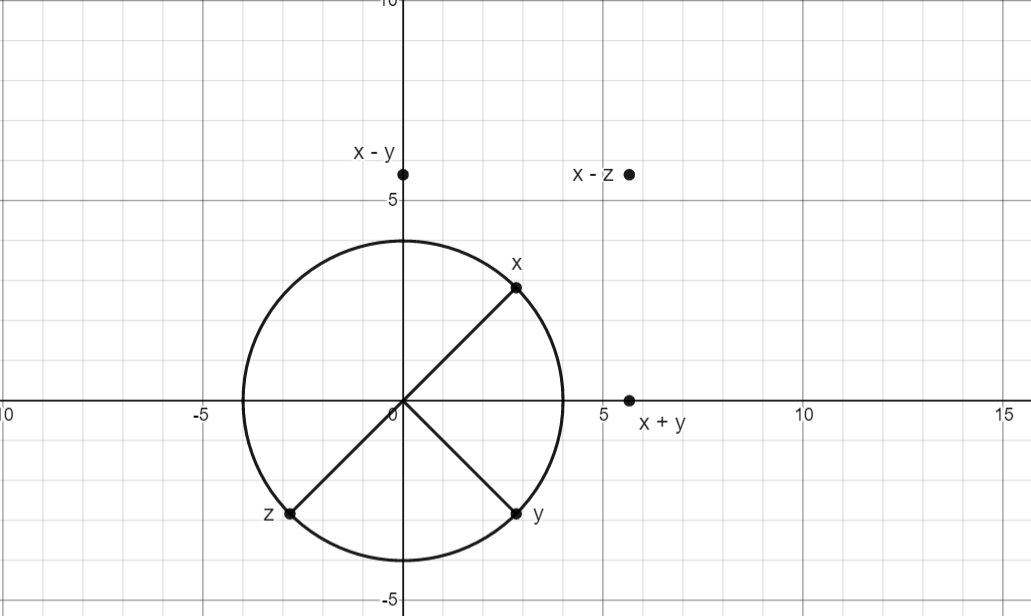
\includegraphics[width=\linewidth]{\resourceDir/img/Analysis/bounded_subset_of_Rm_centred_on_the_origin.png}    
				\caption{A bounded subset of $\R{m}$ centred on the origin.}
				\label{fig:bounded-subset-of-Rm-around-origin}  
			\end{minipage}
			  
			\vspace{0.75cm}
			\begin{minipage}{0.9\textwidth} 
				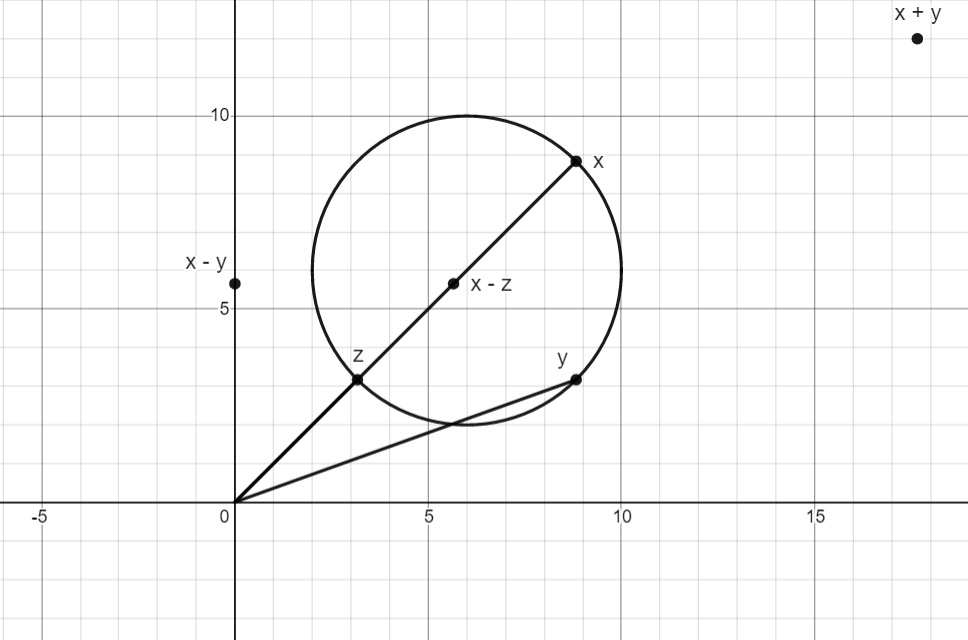
\includegraphics[width=\linewidth]{\resourceDir/img/Analysis/bounded_subset_of_Rm_not_centred_on_the_origin.png}    
				\caption{A bounded subset of $\R{m}$ not centred on the origin.}
				\label{fig:bounded-subset-of-Rm-not-around-origin}   
			\end{minipage}			
		\end{figure}

		\biggerskip
		\labeledProposition{A subset $B$ of $\R{m}$ is bounded iff
			\[ \exists M \geq 0 \in \R{} \logicsep \forall \x \in B \logicsep \norm{\x} \leq M. \]
		}{bounded-subset-contains-bounded-length-vectors}
		\begin{proof}
			Using the unique additive inverse of a vector (\autoref{prop:unique_additive_inverse}) and the general norm properties (\autoref{prop:norm-properties}), for any ${ \x,\y \in \R{m} }$,
			\[\begin{aligned}
				&& \norm{\x} &= \norm{\x - \y + \y} &\sidecomment{by additive inverse of vectors}\\
				&\iff & \norm{\x} &\leq \norm{\x - \y} + \norm{\y} &\sidecomment{by triangle inequality of norms} \\
				&\iff & \norm{\x} - \norm{\y} &\leq \norm{\x - \y}  &(1)
			\end{aligned}\]
			and
			\[\begin{aligned}
				&& \norm{\x - \y} &= \norm{\x + (-\y)} &\sidecomment{by additive inverse of vectors}\\
				&\iff & \norm{\x - \y} &\leq \norm{\x} + \norm{-\y} &\sidecomment{by triangle inequality of norms} \\
				&\iff & \norm{\x - \y} &\leq \norm{\x} + \abs{-1}\norm{\y} &\sidecomment{by norm properties} \\
				&\iff & \norm{\x - \y} &\leq \norm{\x} + \norm{\y}.  &(2)
			\end{aligned}\]
			\nl
			If, ranging over ${ \x \in B }$, $\norm{\x}$ is unbounded then, for some fixed $\y$ and $\norm{\y}$, ${ \norm{\x} - \norm{\y} }$ is unbounded. But then (1) tells us that ${ \norm{\x - \y} }$ is also unbounded. Therefore, the definition of a bounded subset of $\R{m}$ (\ref{def:bounded-subset-of-euclidean-m-space}) implies the proposition,
			\[ \exists M \logicsep \forall \x,\y \in B \logicsep \norm{\x - \y} \leq M \; \implies \; \exists K \logicsep \forall \x \in B \logicsep \norm{\x} \leq K. \]
			Conversely, if $\norm{\x}$ is bounded by a constant $K$ then ${ \norm{\x} + \norm{\y} }$ is bounded by $2K$. Then (2) allows us to deduce that the proposition also implies the definition of a bounded subset of $\R{m}$,
			\[ \norm{\x - \y} \leq \norm{\x} + \norm{\y} \leq 2K \; \implies \; \exists M = 2K \logicsep \forall \x,\y \in B \logicsep \norm{\x} + \norm{\y} \leq M. \]
		\end{proof}
	
	
	
		\biggerskip
		\subheading{Convergence of Sequences in $\R{m}$}
		\nl[6]
		\boxeddefinition{\textbf{(Sequence Convergence in $\R{m}$)} Sequence convergence in $\R{m}$ is similar to convergence in $\R{}$ except that the absolute value becomes the vector norm. So, the sequence $(\x_n)$ \textit{tends to} $\y$ iff
			\[ \forall \epsilon > 0 \in \R{} ,\, \exists N \in \N{} \suchthat \forall n > N ,\, \norm{\x_{n} - \y} < \epsilon. \]
		\label{def:seq-tends-to-y-in-Rm}}
	
		\boxeddefinition{\textbf{(Neighbourhood in $\R{m}$)} The \textit{\mbox{$\epsilon$-neighbourhood of $\y$}} in $\R{m}$ is similar to a bounded subset (\ref{def:bounded-subset-of-euclidean-m-space}) except that it's open. That's to say, it's the set $B$ such that,		
			\[ \exists \epsilon \geq 0 \in \R{} \logicsep \forall \x \in B \logicsep \norm{\x - \y} < \epsilon. \]
		}
		
		\boxeddefinition{\textbf{(Sequence Divergence in $\R{m}$)} A sequence $(\x_n)$ in $\R{m}$ diverges to infinity if
			\[ \forall M > 0 \in \R{} ,\, \exists N \in \N{} \suchthat \forall n > N ,\, \norm{x_{n}} > M. \]
			That's to say, any set that contains the sequence is unbounded and, conversely, any sequence in a bounded set cannot exhibit this behaviour.\\
			
			A sequence in $\R{m}$ may also oscillate boundedly without converging on any point (in this case the sequence would be divergent and yet contained within a bounded set) but unbounded oscillation would come under the concept of diverging to infinity as the norm is non-negative and goes to infinity in this case.\\
			
			\question{Is the concept of divergence in $\R{m}$ actually used in practice?}
		\label{def:seq-diverges-in-Rm}}
		
		\note{A mnemonic for the taxonomy of convergence/divergence behaviours in $\R{m}$. Note that there are fewer classes of behaviour because we use the non-negative norm.\\\\
			\begin{tabular}[h!]{|c|c|c|}
				\cline{1-3}
				convergent & \multicolumn{2}{c|}{divergent}\\
				\cline{1-3}
				bounded & bounded & unbounded \\
				\cline{2-3}
				& oscillatory & ${ \to \infty }$ \\
				\cline{1-3}			
			\end{tabular}
		}
	
		\notation{For a sequence $(\x_n)$ in $\R{m}$, denote the $m$ components of the $n$-th term of the sequence $\x_n$ as ${ x_{1n}, x_{2n}, \dots, x_{mn} }$.}
	
		\biggerskip
		\labeledProposition{A sequence $(\x_n)$ in $\R{m}$ converges to ${ \y \in \R{m} }$ iff each sequence $(x_{in})$ converges to $y_i$ for ${ 1 \leq i \leq m }$.
		}{seq-in-Rm-converges-iff-every-component-converges-to-same-point}
		\begin{proof}
			For any ${ n \in \N{} }$,
			\[ \norm{\x_n - \y} = \sqrt{ (x_{1n} - y_1)^2 + (x_{2n} - y_2)^2 + \cdots + (x_{mn} - y_m)^2 }. \]
			Let
			\[ \epsilon_{max} = \max_{1 \leq i \leq m} x_{in} - y_i. \]
			Then
			\[\begin{aligned}
				&& \norm{\x_n - \y} &\leq \sqrt{m\, {\epsilon_{max}}^2} \nn
				&\iff & \norm{\x_n - \y} &\leq \sqrt{m}\, \epsilon_{max}.
			\end{aligned}\]
			If each sequence $(x_{in})$ converges to $y_i$ then, for all ${ \epsilon > 0 \in \R{} }$, there exists some $N$ such that
			\[ \forall n > N \in \N{} \logicsep \epsilon_{max} < \frac{\epsilon}{\sqrt{m}} \; \implies \; \norm{\x_n - \y} < \epsilon \]
			so $(\x_n)$ converges to $\y$.\\
			
			Conversely, the norm of a vector is greater than or equal to the norm of each component. So, if ${ \norm{\x_n - \y} < \epsilon }$ for some ${ \epsilon }$, then
			\[ \epsilon_{max} \leq \norm{\x_n - \y} < \epsilon \]
			and so for ${ 1 \leq i \leq m }$
			\[ \norm{x_{in} - y_i} < \epsilon \]
			which shows that convergence of $\x_n$ to $\y$ implies convergence of each $x_{in}$ to each $y_i$.
		\end{proof}


% -------------- break ----------------
\pagebreak


	\searchableSubsection{Series}{analysis, real analysis}{
		\bigskip
		\boxeddefinition{\textbf{(Series)} Let $(a_n)_{n=1}^\infty$ be a sequence and let, for ${ n \in \N{} }$,
			\[ s_n = a_1 + a_2 + \cdots + a_n = \sum_{i=1}^n a_i \]
			be the $n$-th partial sum of the terms of the sequence $(a_n)_{n=1}^\infty$. Then, the sequence $(s_n)_{n=1}^\infty$ is called a \textit{series}, denoted $\sum a_n$, with $n$-th term $a_n$ and $n$-th partial sum $s_n$.
		}
		\boxeddefinition{\textbf{(Series Convergence)} A series $\sum a_n$ is \textit{convergent} iff the sequence of partial sums $(s_n)_{n=1}^\infty$ is convergent and divergent iff the sequence of partial sums is divergent.\\
			
		If this sequence converges to a finite value $L$ we say that the \textit{series converges to $L$} or the series \textit{has sum $L$}.
		}\label{def:series-convergence}
	
		\boxeddefinition{\textbf{(Series Rearrangement)} A \textit{rearrangement} of a series ${ \sum a_n }$ is a series ${ \sum a_{f(n)} }$ where $f$ is a permutation of $\N{}$. In other words, the rearrangement contains the same terms as the original series but appearing in a different order.}
	
		\boxeddefinition{\textbf{(Non-negative Series)} A series is described as \textit{non-negative} if all its terms are non-negative. That's to say, the sequence $\sum a_n$ is non-negative iff
			\[ \forall n \in \N{} \logicsep a_n \geq 0. \]
		}\label{def:non-negative-series}
	
		\boxeddefinition{\textbf{(Alternating Series)} A series is described as \textit{alternating} if its terms are alternately positive and negative.}
		
		\notation{The series $(s_n)_{n=1}^\infty$ with $n$-th term $a_n$ is typically denoted ${ \sum a_n }$ but some authors use the notation ${ \sum_{n=1}^\infty a_n }$ which has the disadvantage that it may be confused with the sum to infinity of the series (which may or may not exist depending on whether the series converges).}
		
		\note{A series may also be finite but finite series necessarily converge and so are not a subject of study in Analysis (but may be studied in Calculus).}
	
	
	
		\biggerskip
		\labeledProposition{If a series $\sum a_n$ converges then the terms ${ a_n \to 0 }$ as ${ n \to \infty }$.}{convergent-series-has-terms-that-go-to-0}
		\begin{proof}
			Let ${ f: \N{}\longmapsto \N{} }$ be defined as
			\[ f(n) = n-1. \]
			Then $f$ is a strictly increasing function over the naturals and so, by the definition \ref{def:subsequence}, $(s_{f(n)})$ is a subsequence of the sequence of partial sums $(s_n)$ of the series $\sum a_n$. By \autoref{prop:subseq-tends-to-same-limit} then, the subsequence $(s_{f(n)})$ tends to the same limit as $(s_n)$.\\
			Since both sequences tend to some finite limit $L$, we can use \autoref{prop:func-finite-limit-algebra} to evaluate the limit,
			\[ \lim_{n \to \infty} (s_{f(n)} - s_n) = L - L = 0. \]
			Since ${ f(n) = n-1 }$, it follows that
			\[ (s_{f(n)} - s_n) = (s_{n-1} - s_n) = a_n \]
			and so
			\[ \lim_{n \to \infty} (s_{f(n)} - s_n) = \lim_{n \to \infty} a_n = 0.  \qedhere \]
		\end{proof}
	
	
		\bigskip
		\labeledProposition{\textbf{(Algebra of Series)} Let ${ \sum a_n }$ be a series that converges to $L$ and ${ \sum b_n }$ be a series that converges to $M$. Then for any real number $C$,
			\begin{enumerate}[label=(\roman*)]
				\item{${ \sum_{n=1}^\infty C a_n = C L }$}
				\item{${ \sum_{n=1}^\infty (a_n + b_n) = L + M }$}
			\end{enumerate}
		}{series-limit-algebra}
		\begin{proof}\nl
			\begin{enumerate}[label=(\roman*)]
				\item Let
					\[ s_n = \sum_{i=1}^n a_i \]
					be the $n$-th partial sum of ${ \sum a_n }$. Then
					\[ t_n = \sum_{i=1}^n C a_i = C \sum_{i=1}^n a_i = C s_n. \]
					Using \autoref{prop:func-finite-limit-algebra}, we can therefore deduce
					\[ \lim_{n \to \infty} s_n = L \implies \lim_{n \to \infty} t_n = \lim_{n \to \infty} C s_n = C L.  \]
				
				\bigskip
				\item Let
					\[ s_n = \sum_{i=1}^n a_i, t_n = \sum_{i=1}^n b_i \]
					be the $n$-th partial sums of ${ \sum a_n }$ and ${ \sum b_n }$ respectively.
					Then
					\[ u_n = \sum_{i=1}^n a_i + b_i = \sum_{i=1}^n a_i + \sum_{i=1}^n b_i = s_n + t_n \]
					and we can use \autoref{prop:func-finite-limit-algebra} to deduce
					\[ \lim_{n \to \infty} u_n = \lim_{n \to \infty} s_n + t_n = L + M. \]
			\end{enumerate}
		\end{proof}
		\note{Note that linear combinations of series conform to the algebra of (finite) limits of sequences \autoref{prop:func-finite-limit-algebra}; which is to be expected as the series is a sum of the terms of a sequence. Also, as expected, due to the lack of distributivity of addition over multiplication, the series algebra does not work for products --- e.g. if ${ \sum a_n }$ and ${ \sum b_n }$ converge then it does \textbf{not} follow that the product series ${ \sum a_n b_n }$ converges (see: \ref{ex:absolutely-convergent-series-whose-square-diverges}).}
	
	
		\biggerskip
		\subsubsection{Non-negative Series}
		{\tiny 
			\hyperref[ssssection:well-known-non-negative-series]{Well-Known Series} \hspace{20pt} \hyperref[ssssection:convergence-tests-for-non-negative-series]{Convergence Tests}
		}
		\biggerskip
		\labeledProposition{If a series is non-negative then its partial sums are monotonically increasing.}{non-negative-series-is-monotonically-increasing}
		\begin{proof}
			Let $s_n$ be the $n$-th partial sum of the sequence $\sum a_n$. For all $n$, 
			\[ a_n \geq 0 \implies s_n - s_{n-1} \geq 0 \iff s_n \geq s_{n-1}. \]
			Therefore, the sequence of partial sums $(s_n)_{n=1}^\infty$ is monontonically increasing. 
		\end{proof}
				
		\bigskip
		\labeledProposition{If a series $\sum a_n$ is non-negative (\ref{def:non-negative-series}), then either the series converges or it goes to infinity. That's to say, if the series diverges, then the $n$-th partial sum ${ s_n \to \infty }$ as ${ n \to \infty }$.}{non-negative-series-either-converges-or-goes-to-infinity}
		\begin{proof}
			By \autoref{prop:non-negative-series-is-monotonically-increasing}, the sequence of $n$-th partial sums $(s_n)$ is increasing. In addition, the sequence either has an upper bound or it does not. By \autoref{prop:increasing_bounded_seqs_have_limit}, if it has an upper bound then it converges which, by the definition \ref{def:series-convergence}, is to say that the sequence $\sum a_n$ converges.\\
			
			Alternatively, if does not have an upper bound then
			\[ \forall K \in \R{} \logicsep \exists N \logicsep \forall n > N \in \N{} \logicsep s_n > K \]
			which, by the definition \ref{def:seq-diverges}, is to say that ${ \lim_{n \to \infty} s_n = \infty }$.
		\end{proof}
	
	
		
		\nl[20]
		\subsubsubsection{Well-known Non-negative Series}\label{ssssection:well-known-non-negative-series}
		\medskip
		\labeledTheorem{\textbf{(Geometric Series)} Let ${ a, r \in \R{} }$. Then the series ${ \sum ar^{n-1} }$,
			\begin{enumerate}[label=(\roman*)]
				\item{converges to ${ \frac{1}{a-r} }$ if ${ \abs{r} < 1 }$;}
				\item{diverges if ${ \abs{r} \geq 1 }$.}
			\end{enumerate}
		}{geometric-series-convergence-conditions}
		\begin{proof}\nl
			The sum of a geometric progression, for ${ r = 1 }$ is given by ${ s_n = na }$ and, for ${ r \neq 1 }$, is given by
			\[ s_n = \frac{ar^n - a}{r - 1} = \frac{a}{r - 1} (r^n - 1). \]
			So, the limit of this sum as ${ n \to \infty }$ is given by,
			\[ \lim_{n \to \infty} s_n = \lim_{n \to \infty} \frac{a}{r - 1} (r^n - 1) = \frac{a}{r - 1} \lim_{n \to \infty} (r^n - 1). \]
			Then, by \autoref{prop:geometric-progression-sequence-diverges-or-converges-to-0-or-initial-value},
			\begin{enumerate}[label=(\roman*)]
				\item{if ${ \abs{r} < 1 }$, then
					\[ \lim_{n \to \infty} r^n = 0 \implies \lim_{n \to \infty} (r^n - 1) = -1 \implies \lim_{n \to \infty} s_n = -\frac{a}{r - 1} = \frac{a}{1 - r}. \]
				}
				\item{if ${ \abs{r} \geq 1 }$, then either:
					\begin{itemize}
						\item{${ \abs{r} > 1 }$ and so
							\[ \lim_{n \to \infty} r^n \text{ diverges } \implies \lim_{n \to \infty} s_n \text{ diverges, } \]
							\note{if ${ r < -1 }$, the sequence $(r^n)$ oscillates unboundedly}
						}
						\item{${ \abs{r} = 1 \iff r \in \{-1, 1\} }$ and, if ${ r = 1 }$ then
							\[ \lim_{n \to \infty} s_n = \lim_{n \to \infty} na = a \lim_{n \to \infty} n = \infty \]
							or else ${ r = -1 }$ and ${ \lim_{n \to \infty} r^n = \lim_{n \to \infty} (-1)^n }$ which alternates between -1 and 1 and so diverges in a bounded oscillatory fashion.
						}
					\end{itemize}
				}
			\end{enumerate}
		\end{proof}
	
	
		\bigskip
		\labeledTheorem{\textbf{Harmonic Series} The harmonic series ${ \sum \frac{1}{n} }$ diverges.}{harmonic-series-diverges}
		\begin{proof}\nl[2]
			Let ${ s_n = \sum_{i=1}^n \frac{1}{i} }$ be the $n$-th partial sum of the series ${ \sum \frac{1}{n} }$ and let ${ f: \N{} \longmapsto \N{} }$ be the monotonically increasing function,
			\[ f(n) = 2^{n-1} n \]
			so that $(s_{f(n)})$ is a subsequence of $(s_n)$.\\
			
			Suppose, for contradiction, that $(s_n)$ converges to a finite limit $L$. Then, by \autoref{prop:subseq-tends-to-same-limit}, $(s_{f(n)})$ also converges to $L$ and so, by \autoref{prop:convergent-series-has-terms-that-go-to-0},
			\[ \lim_{n \to \infty} (s_{f(n)} - s_{f(n-1)}) = 0. \tag{*} \]
			\nl
			If we expand out the expression ${ s_{f(n)} - s_{f(n-1)} }$, we can deduce that, for all ${ n \in \N{} }$,
			\[\begin{aligned}
				s_{f(n)} - s_{f(n-1)} &= s_{2m} - s_m  &\sidecomment{for some ${ m \in \N{} }$} \nn
				&= \sum_{i=1}^{2m} \frac{1}{i} - \sum_{i=1}^m \frac{1}{i} &\sidecomment{} \nn
				&= \sum_{i=m+1}^{2m} \frac{1}{i} &\sidecomment{} \nn
				&= \frac{1}{m+1} + \frac{1}{m+2} + \cdots + \frac{1}{2m} &\sidecomment{} \nn
				&> \frac{1}{2m} + \frac{1}{2m} + \cdots + \frac{1}{2m} = \frac{m}{2m} = \frac{1}{2}.
			\end{aligned}\]
			\nl
			But by \autoref{prop:if-a-seq-is-geq-M-and-converges-to-L-then-L-is-geq-M} we have
			\[ \forall n \logicsep (s_{f(n)} - s_{f(n-1)}) \geq \frac{1}{2} \implies \lim_{n \to \infty} (s_{f(n)} - s_{f(n-1)}) \geq \frac{1}{2} \]
			which contradicts (*).\\
			
			Therefore, the series diverges.
		\end{proof}
		\note{Compare with 
			\[ \int_a^{ab} \frac{1}{t} \dif t = \int_1^b \frac{a}{au} \dif u= \int_1^b \frac{1}{u} \dif u = \ln(b) \]
			which is to say that the value of integral of $1/t$ between $a$ and $ab$ doesn't depend on the value of $a$. In other words, if the interval of integration is from some $x$ to $cx$ for constant $c$, then the value of the integral is ${ \ln(c) }$.
		}
	
		\bigskip
		\labeledProposition{The series ${ \sum \frac{1}{n^k} }$,
			\begin{enumerate}[label=(\roman*)]
				\item diverges if ${ k \leq 1 }$;
				\item converges if ${ k > 1 }$.
			\end{enumerate}
		}{series-n-exp-minus-k-diverges-if-k-leq-1-and-converges-if-k-gt-1}
		\begin{proof}\nl
			Let $(s_n)$ be the sequence of partial sums of ${ \sum 1/n^k }$.
			\begin{enumerate}[label=(\roman*)]
				\item Assume ${ k \leq 1 \in \R{} }$. Then, for all ${ n \in \N{} }$,
				\[ n^k < n \iff \frac{1}{n^k} > \frac{1}{n}. \]
				Furthermore, since both ${ \sum 1/n }$ and ${ \sum 1/n^k }$ are non-negative series, by \autoref{prop:non-negative-series-either-converges-or-goes-to-infinity}, they can only converge to a finite limit or go to infinity. By \autoref{theo:harmonic-series-diverges}, the harmonic series ${ \sum 1/n }$ goes to infinity. Therefore, ${ \sum 1/n^k }$ must be unbounded and also go to infinity.
				
				\bigskip
				\item Assume ${ k > 1 }$. The series ${ \sum 1/n^k }$ is non-negative and so it is monotonically increasing (\autoref{prop:non-negative-series-is-monotonically-increasing}). It follows then that
				 \[ 2^n - 1 \geq n \implies s_{2^n - 1} \geq s_n \]
				 and so the subsequence $(s_{2^n - 1})$ is an upper bound on the sequence $(s_n)$. If $(s_{2^n - 1})$ is upper bounded then this will imply that $(s_n)$ is upper bounded and then, by \autoref{prop:increasing_bounded_seqs_have_limit}, $(s_n)$ must converge.\\
				 
				 Consider the partial sums of $(s_{2^n - 1})$,
				 \[\begin{aligned}
				 	s_{2^n - 1} &= \sum_{i=1}^{2^n - 1} \frac{1}{i^k} \nnn
				 	&= \frac{1}{1^k} + \frac{1}{2^k} + \cdots + \frac{1}{(2^n - 1)^k} &\sidecomment{} \nnn
				 	&= 1 + \left(\frac{1}{2^k} + \frac{1}{3^k}\right) + \left(\frac{1}{4^k} + \frac{1}{5^k} + \frac{1}{6^k} + \frac{1}{7^k}\right) + \cdots \nn
				 	&\hspace{20pt} + \left(\frac{1}{(2^{n-1})^k} + \frac{1}{(2^{n-1} + 1)^k} + \cdots + \frac{1}{(2^n - 1)^k}\right) &\sidecomment{} \\
				 \end{aligned}\]
			 	 where we have grouped terms into groups of $1, 2, 4, 8, \dots, 2^{n-1}$ terms. The sum of each such group is of the form, for ${ m \in \N{} \cup \{0\} }$,
			 	 \[ \frac{1}{(2^m + 0)^k} + \frac{1}{(2^m + 1)^k} + \cdots + \frac{1}{(2^m + (2^m - 1))^k} \leq \frac{2^m}{(2^m)^k} = \frac{1}{2^{m(k-1)}}. \]
			 	 Therefore, if we let ${ t_n =  }$
			 	 \[\begin{aligned}
			 	 	s_{2^n - 1} &\leq \sum_{m=0}^{n-1} \frac{1}{2^{m(k-1)}} \nn
			 	 	&= \frac{\frac{1}{2^{n(k-1)}} - 1}{\frac{1}{2^{(k-1)}} - 1}
			 	 \end{aligned}\]
		 	 	\nl
		 	 	and the limit as ${ n \to \infty }$ of this upper bound on $s_{2^n - 1}$ is
		 	 	\[ \lim_{n \to \infty} \frac{\frac{1}{2^{n(k-1)}} - 1}{\frac{1}{2^{(k-1)}} - 1} = \frac{0 - 1}{\frac{1}{2^{(k-1)}} - 1} = \frac{1}{1 - \frac{1}{2^{(k-1)}}} = \frac{1}{1 - 2^{(1-k)}}. \]
		 	 	So we have found a convergent sequence that is an upper bound on $(s_{2^n - 1})$ and so $(s_{2^n - 1})$ is upper bound and, therefore, $(s_n)$ converges.
			\end{enumerate}
		\end{proof}
	
		
		
		\nl[20]
		\subsubsubsection{Convergence Tests for Non-negative Series}\label{ssssection:convergence-tests-for-non-negative-series}
		\bigskip
		\labeledTheorem{\textbf{(Comparison Test)} Suppose $(a_n)$ and $(b_n)$ are non-negative sequences. Then:
			\begin{enumerate}[label=(\roman*)]
				\item If ${ a_n \leq b_n }$ for all ${ n \in \N{} }$, then
					\begin{itemize}
						\item if ${ \sum b_n }$ converges then ${ \sum a_n }$ converges and 
							\[ \sum_{n=1}^\infty a_n \leq \sum_{n=1}^\infty b_n, \]
						\item if ${ \sum a_n }$ diverges then ${ \sum b_n }$ diverges;
					\end{itemize}
				\bigskip
				\item If there exists some $N$ such that ${ a_n \leq b_n }$ for all ${ n > N \in \N{} }$, then
					\begin{itemize}
						\item if ${ \sum b_n }$ converges then ${ \sum a_n }$ converges,
						\item if ${ \sum a_n }$ diverges then ${ \sum b_n }$ diverges;
					\end{itemize}
				\bigskip
				\item If 
					\[ L = \lim_{n \to \infty} \frac{a_n}{b_n} \]
					is finite and non-zero, then
					\[ \sum a_n \text{ converges } \iff \sum b_n \text{ converges. } \]
			\end{enumerate}
		}{series-comparison-test}
		\begin{proof}\nl
			Let $s_n$ and $t_n$ be the $n$-th partial sums of ${ \sum a_n }$ and ${ \sum b_n }$ respectively. Since the terms $a_n$ and $b_n$ are non-negative, by \autoref{prop:non-negative-series-is-monotonically-increasing}, the sequences $(s_n)$ and $(t_n)$ are monotonically increasing.
			\begin{enumerate}[label=(\roman*)]
				\item Assume ${ a_n \leq b_n }$ for all ${ n \in \N{} }$. Then
					\[ s_n = \sum_{i=1}^n a_n \leq \sum_{i=1}^n b_n = t_n \]
					which is to say that $t_n$ is an upper bound for $s_n$. Since ${ \sum b_n }$ converges, by definition $t_n$ converges. Since $t_n$ converges, by \autoref{prop:convergent_seqs_bounded} it is bounded, and in particular, upper bounded. The upper bound on $t_n$ must transitively be an upper bound on $s_n$ also. Then, since $(s_n)$ is monotonically increasing, by \autoref{prop:increasing_bounded_seqs_have_limit}, $(s_n)$ is convergent. Furthermore, by \autoref{coro:increasing-seq-bounded-above-converges-to-supremum},
					\[ \lim_{n \to \infty} t_n = \sup \setc{t_n}{n \in \N{}} \leq \sup \setc{s_n}{n \in \N{}} = \lim_{n \to \infty} s_n. \]
					\nl
					If, on the other hand, ${ \sum a_n }$ diverges, by the increasing property and \autoref{prop:non-negative-series-either-converges-or-goes-to-infinity}, it must go to infinity (which is to say that the partial sums $s_n$ go to infinity). Therefore, the partial sums $t_n$ must also go to infinity and so, by definition, ${ \sum b_n }$ diverges also.
				\bigskip
				\item Assume there exists some $N$ such that ${ a_n \leq b_n }$ for all ${ n > N \in \N{} }$. Then
					\[ \sum_{i=N+1}^n a_n \leq \sum_{i=N+1}^n b_n. \]
					Let
					\[ s_N = \sum_{i=1}^N a_n \eqand t_N = \sum_{i=1}^N b_n. \]
					So we have,
					\[ s_n = s_N + \sum_{i=N+1}^n a_n \eqand t_n = t_N + \sum_{i=N+1}^n b_n \]
					and then it follows that
					\[\begin{aligned}
						&& \sum_{i=N+1}^n a_n &\leq \sum_{i=N+1}^n b_n \nn
						&\iff & s_N + \sum_{i=N+1}^n a_n &\leq s_N + \sum_{i=N+1}^n b_n \nn
						&\iff & s_n &\leq t_n - t_N + s_N \nn
						&\iff & s_n &\leq t_n + (s_N - t_N).
					\end{aligned}\]
					In a similar fashion to (i): Convergence of the series $\sum b_n$ implies that the sequence $(t_n)$ converges, which by \autoref{prop:convergent_seqs_bounded}, implies that it is upper bounded. Since ${ s_N - t_N }$ is some constant, the upper bound on $t_n$ means that $s_n$ also has an upper bound, and, being monotonically increasing, by \autoref{prop:increasing_bounded_seqs_have_limit}, is therefore convergent.\\
					
					If ${ \sum a_n }$ diverges on the other hand, then by \autoref{prop:non-negative-series-either-converges-or-goes-to-infinity}, we have
					\[ \lim_{n \to \infty} s_n = \infty \implies \lim_{n \to \infty} [t_n + (s_N - t_N)] = \infty \implies \lim_{n \to \infty} t_n = \infty \]
					which is to say that ${ \sum b_n }$ diverges.
				\bigskip
				\item Suppose we have
					\[ L = \lim_{n \to \infty} \frac{a_n}{b_n}. \]
					Then, by the definition of the limit of sequences (\ref{def:seq-tends-to-L}), for all ${ \epsilon > 0 \in \R{} }$, there exists some $N$ such that,
					\[ \forall n > N \logicsep \abs{\frac{a_n}{b_n} - L} < \epsilon \]
					which is to say
					\[ L - \epsilon < \frac{a_n}{b_n} < \epsilon + L. \]
					Let ${ K \in \R{} }$ be a constant such that ${ K = \epsilon + L }$. Then,
					\[ a_n < K b_n \eqand b_n < \frac{1}{K} a_n \]
					for all ${ n > N \in \N{} }$. If ${ \sum b_n }$ converges then by the algebra of series (\autoref{prop:series-limit-algebra}), ${ \sum K b_n }$ also converges and we can apply (ii) to deduce that ${ \sum a_n }$ converges also. Similarly, if ${ \sum a_n }$ converges then ${ \sum \frac{1}{K} a_n }$ converges and applying (ii) we obtain the result that ${ \sum b_n }$ converges also.
			\end{enumerate}
		\end{proof}
	
	
		\bigskip
		\labeledTheorem{\textbf{(Ratio Test)} Let ${ \sum a_n }$ be a non-negative series with the property that
			\[ L = \lim_{n \to \infty} \frac{a_{n+1}}{a_n} \]
			where $L$ may be infinity. Then,
			\begin{enumerate}[label=(\roman*)]
				\item ${ L < 1 \implies \sum a_n \text{ converges, } }$
				\item ${ L > 1 \implies \sum a_n \text{ diverges. } }$
			\end{enumerate}
		}{series-ratio-test}
		\begin{proof}
			\nl
			\begin{enumerate}[label=(\roman*)]
				\item In the case that ${ L < 1 }$, there exists some $N$ such that, for all ${ n > N \in \N{} }$ and ${ \epsilon < 1 - L }$,
				\[ \abs{\frac{a_{n+1}}{a_n} - L} < \epsilon \iff L - \epsilon < \frac{a_{n+1}}{a_n} < L + \epsilon. \]
				Let ${ r = \epsilon + L }$. Then,
				\[ \frac{a_{n+1}}{a_n} < r \iff a_{n+1} < r a_n \]
				with ${ 0 < r < 1 }$. Therefore, the sum of the terms after $N$,
				\[ \sum_{i=N+1}^\infty a_i <  \sum_{i=1}^\infty r^i a_N \]
				which is a geometric series with absolute common ratio less than one. Therefore, by \autoref{theo:geometric-series-convergence-conditions}, the sum of the terms after $N$ is convergent and finite and since, the sum of the finite number of terms upto $N$ is necessarily finite also, we conclude that the series converges. Since this is a convergent upper bound on ${ \sum a_n }$, by \autoref{theo:series-comparison-test}, ${ \sum a_n }$ converges.
				\medskip
				\item In the case that ${ L > 1 }$, we can use a similar argument to show that the sequence ${ \sum a_n }$ is lower bounded by a geometric sequence with absolute common ratio greater than 1 so that \autoref{theo:geometric-series-convergence-conditions} tells us that this lower bound diverges. Then, again applying the \autoref{theo:series-comparison-test}, ${ \sum a_n }$ diverges.
			\end{enumerate}
		\end{proof}
		\note{Note that the Ratio Test makes no inference if the limit of the ratio of consecutive terms is equal to 1. In this case the series may or may not converge. For example, ${ \sum 1/n }$ and ${ \sum 1/n^2 }$ both have a ratio of consecutive terms that tends to 1 but the first diverges while the second converges.}
		
		\bigskip
		\labeledTheorem{\textbf{(Root Test)} Let ${ \sum a_n }$ be a non-negative series with the property that
			\[ L = \lim_{n \to \infty} {a_n}^{1/n} \]
			where $L$ may be infinity. Then,
			\begin{enumerate}[label=(\roman*)]
				\item ${ L < 1 \implies \sum a_n \text{ converges, } }$
				\item ${ L > 1 \implies \sum a_n \text{ diverges. } }$
		\end{enumerate}}{series-root-test}
		\begin{proof}\nl
			\begin{enumerate}[label=(\roman*)]
				\item Assume ${ L < 1 }$ so that for some ${ 0 < r < 1 }$,
				\[ \lim_{n \to \infty} {a_n}^{1/n} < 1 \implies \exists N \logicsep \forall n > N \logicsep {a_n}^{1/n} < r \]
				which is to say that ${ a_n < r^n }$ and therefore the series ${ \sum a_n }$ is upper bounded by the series ${ \sum r^n }$. Since ${ \abs{r} < 1 }$, by \autoref{theo:geometric-series-convergence-conditions}, the series ${ \sum r^n }$ converges and so by \autoref{theo:series-comparison-test}, ${ \sum a_n }$ converges also.
				
				\bigskip
				\item Similarly, if ${ L > 1 }$ we can lower bound the series ${ \sum a_n }$ with a geometric series with common ratio ${ \abs{r} > 1 }$ and, using \autoref{theo:geometric-series-convergence-conditions}, deduce that this lower bound series diverges which, since it is a non-negative series, by \autoref{prop:non-negative-series-either-converges-or-goes-to-infinity}, means that the partial sums go to infinity. Therefore the partial sums of ${ \sum a_n }$ also go to infinity. 
			\end{enumerate}			
		\end{proof}
	
		\bigskip
		\labeledTheorem{\textbf{(Integral Test)} Let ${ a \geq 1 \in \R{} }$ and ${ f: \R{} \longmapsto \R{} }$ be a positive, decreasing, integrable function on ${ [a, \infty) }$. Then the series ${ \sum f(n) }$ converges iff the improper integral ${ \int_a^\infty f(t) \dif t }$ exists.}{series-integral-test}
		\begin{proof}
			Denote $n$-th partial sum of ${ \sum f(n) }$, $s_n$. Then
			\[ s_n = \sum_{i=1}^n f(i). \]
			By the definition of the Riemmann Integral \ref{def:riemann-integral} and the upper and lower estimates used in the definition \ref{def:lower-and-upper-estimates-of-area-under-curve}, since $f$ is a decreasing function, the upper estimate of the integral ${ \int_a^b f(t) \dif t }$ --- for some ${ b > a \in \R{} }$ --- over the partition ${ P = \{ a+1, a+2,\dots, b\} }$ is
			\[ U(P) = \sum_{i=a}^{b-1} (x_{i+1} - x_i) \max_{ x_i \leq x \leq x_{i+1} }{ f(x) }. \]
			But for this partition $P$ we have ${ (x_{i+1} - x_i) = 1 }$ and since $f$ is a decreasing function, for all ${ a \leq i \leq b-1 }$,
			\[ \max_{ x_i \leq x \leq x_{i+1} }{ f(x) } = \max_{ i \leq x \leq i+1 }{ f(x) } = f(i). \]
			So the upper estimate becomes, letting ${ n = b-1 }$,
			\[ U(P) = \sum_{i=a}^{b-1} f(i) = s_n - s_a \]
			the $n$\textsuperscript{th} partial sum minus the $a$\textsuperscript{th} partial sum of the series ${ \sum f(n) }$. Since the upper estimate is, by definition, an upper bound on the value of the integral we therefore have,
			\[ s_n - s_a \geq \int_a^b f(t) \dif t \iff s_n \geq \int_a^b f(t) \dif t + s_a. \]
			Since $f$ is a positive function, the integral ${ \int_a^b f(t) \dif t }$ is positive and so, if $b$ is allowed to go to infinity, then the value of the integral must, by \autoref{prop:non-negative-series-either-converges-or-goes-to-infinity}, either converge to a finite limit or tend to infinity.\\
			If the integral goes to infinity (i.e. the improper integral doesn't exist) then $s_n$, being an upper bound on its value, must also go to infinity. On the other hand, if the integral exists (i.e. it converges to a finite limit) then, by the definition of the Riemann Integral, the upper and lower estimates must converge. Therefore $(s_n)$ converges.
		\end{proof}
	
	
		\biggerskip
		\subsubsection{Absolute and Conditional Convergence}
		\bigskip
		\boxeddefinition{\textbf{(Absolute Convergence)} If a series ${ \sum a_n }$ is such that ${ \sum \abs{a_n} }$ is a convergent series, then the series ${ \sum a_n }$ is described as \textit{absolutely convergent}.\\
		
		Clearly, for non-negative series in which, by definition, ${ \forall n \logicsep a_n = \abs{a_n} }$, convergence implies absolute convergence.}
	
		\boxeddefinition{\textbf{(Conditional Convergence)} If a series ${ \sum a_n }$ is such that ${ \sum \abs{a_n} }$ is a divergent series but the original series ${ \sum a_n }$ is a convergent series, then the series ${ \sum a_n }$ is described as \textit{conditionally convergent}.}
		
		\notation{Let ${ \sum a_n^+ }$ denote the series whose terms are the positive terms of the sequence $a_n$ and, similarly, ${ \sum a_n^- }$ the series of the negative terms of $a_n$.\\
			
		More formally, define
			\[ 	a_n^+ = \begin{cases}
							a_n & a_n > 0 \\
							0   & a_n \leq 0
						\end{cases}  \eqand
				a_n^- = \begin{cases}
							0 & a_n \geq 0 \\
							a_n   & a_n < 0.
						\end{cases}
			\]
		Then we have the following relationships:
			\begin{itemize}
				\item ${ \sum a_n = \sum a_n^+  + \sum a_n^- }$
				\item ${ \sum \abs{a_n} = \sum a_n^+  - \sum a_n^- }$.
			\end{itemize}
		}
		
		\biggerskip
		\labeledProposition{Let ${ \sum a_n }$ be an arbitrary series. Then,
			\begin{enumerate}[label=(\roman*)]
				\item ${ \sum a_n^+ }$ is monotonically increasing and so either converges or diverges to infinity; and
				\item ${ \sum a_n^- }$ is monotonically decreasing and so either converges or diverges to negative infinity.
			\end{enumerate}
		}{series-of-positive-terms-is-increasing-series-of-negative-terms-is-decreasing}
		\begin{proof}
			\begin{enumerate}[label=(\roman*)]
				\item Clearly ${ \sum a_n^+ }$ is a non-negative series and so, by \autoref{prop:non-negative-series-is-monotonically-increasing}, is monotonically increasing and then, by \autoref{prop:increasing_bounded_seqs_have_limit}, either converges or diverges to infinity.
				\item Considering the series ${ \sum a_n^- }$ on the other hand, we have
				\[ \sum a_n^- = -\sum -a_n^- \]
				where $\sum -a_n^-$ is a monotonically increasing sequence and so, by similar reasoning, it follows that $\sum -a_n^-$ either converges or diverges to infinity. Therefore, ${ \sum a_n^- }$ either converges or diverges to negative infinity.
			\end{enumerate}
		\end{proof}
		
		\bigskip
		\labeledProposition{Absolute convergence implies convergence.}{series-absolute-convergence-implies-conditional-convergence}
		\begin{proof}
			\note{Note that the triangle inequality tells us that ${ \sum \abs{a_n} }$ is an upper bound on ${ \sum a_n }$ but because ${ \sum a_n }$ is not a non-negative sequence, convergence of ${ \sum \abs{a_n} }$ does \textbf{not} imply that ${ \sum a_n }$ converges: it may oscillate boundedly (if it oscillated unboundedly then it wouldn't be absolutely convergent).}
			
			Let ${ \sum a_n }$ be an absolutely convergent sequence and consider the series ${ \sum a_n + \abs{a_n} }$. For each term of this series we have,
			\[ 0 <= a_n + \abs{a_n} \leq 2\abs{a_n} \] 
			so ${ \sum (a_n + \abs{a_n}) }$ is a non-negative series upper-bounded by ${ \sum 2\abs{a_n} }$ which is convergent because, by the absolute convergence and the algebra of convergent series (\autoref{prop:series-limit-algebra}), ${ \sum 2\abs{a_n} = 2 \sum \abs{a_n} }$ is convergent. Therefore, by \autoref{prop:non-negative-series-is-monotonically-increasing} and \autoref{prop:increasing_bounded_seqs_have_limit}, ${ \sum (a_n + \abs{a_n}) }$ is convergent.\\
			
			Now, again using the algebra of convergent series, we have, 
			\[ \sum a_n = \sum (a_n + \abs{a_n}) - \sum \abs{a_n} \]
			must be convergent also.
		\end{proof}
		
		\bigskip
		\labeledProposition{A conditionally convergent series doesn't necessarily converge to the same limit after rearrangement.}{conditionally-convergent-series-value-not-invariant-under-rearrangement}
		\begin{proof}
			Consider the Taylor expansion of ${ \ln(1+x) }$,
			\[\begin{aligned}
				\ln(1+x) &= \ln(1) + \left(\dod{\ln}{x}\Bigr\rvert_{x=1}\right) \frac{x}{1!} + \left(\dod[2]{\ln}{x}\Bigr\rvert_{x=1}\right) \frac{x^2}{2!} + \left(\dod[3]{\ln}{x}\Bigr\rvert_{x=1}\right) \frac{x^3}{3!} + \cdots \nnn
				&= 0 + \left(\frac{1}{1}\right) \frac{x}{1!} + \left(\frac{-1}{1^2}\right) \frac{x^2}{2!} + \left(\frac{2}{1^3}\right) \frac{x^3}{3!} + \left(\frac{-3 \times 2}{1^4}\right) \frac{x^4}{4!} + \cdots &\sidecomment{} \nnn
				&= \sum_{n=1}^\infty (-1)^{n+1} \frac{(n-1)!}{n!} x^n = \sum_{n=1}^\infty (-1)^{n+1}\, \frac{x^n}{n}.
			\end{aligned}\]
			\note{Note that we could also have obtained the same result by noting that the sum of an infinite geometric series with initial term 1 and ${ \abs{r} < 1 }$, where $r$ is the common ratio, is given by
				\[ \frac{1}{1 - r}. \]
				If $r$ is negative then we have ${ r = -t }$ for some positive $t$ and,
				\[ \frac{1}{1 + t} = 1 - t + t^2 - t^3 + \cdots \]
				Integrating both sides \wrt $t$ we get,
				\[ \int_1^x \frac{1}{1 + t} \dif t = t - \frac{t^2}{2} + \frac{t^3}{3} - \frac{t^4}{4} + \cdots \]
			}
			So, using this to obtain a series summing to $\ln(2)$, we have
			\[ \ln(2) = \ln(1 + 1) = \sum_n (-1)^{n+1}\, \frac{1}{n} = 1 - \frac{1}{2} + \frac{1}{3} - \frac{1}{4} + \frac{1}{5} - \frac{1}{6} + \frac{1}{7} - \frac{1}{8} + \cdots  \tag{1} \]
			Then, using the algebra of convergent series (\autoref{prop:series-limit-algebra}),
			\[ \frac{1}{2} \ln(2) = \frac{1}{2} \sum_n (-1)^{n+1}\, \frac{1}{n} = \frac{1}{2} - \frac{1}{4} + \frac{1}{6} - \frac{1}{8} + \cdots \]
			and adding in a zero for every odd-numbered term,
			\[ \frac{1}{2} \ln(2) = 0 + \frac{1}{2} + 0 - \frac{1}{4} + 0 + \frac{1}{6} + 0 - \frac{1}{8} + 0 + \cdots  \tag{2} \]
			Now adding (1) and (2),
			\[\begin{aligned}
				&& \ln(2) + \frac{1}{2} \ln(2) &= 1 + 0 + \frac{1}{3} - \frac{1}{2} + \frac{1}{5} + 0 + \frac{1}{7} - \frac{1}{4} + \cdots  \nnn
				& \iff & \frac{3}{2} \ln(2) &= 1 + \frac{1}{3} - \frac{1}{2} + \frac{1}{5} + \frac{1}{7} - \frac{1}{4} + \cdots
			\end{aligned}\]
			Here we have obtained an expression that the algebra of convergent series tells us evaluates to ${ \frac{3}{2} \ln(2) }$ but that is clearly a rearrangement of (1) which we know converges to ${ \ln(2) }$.\\
			Note also that (1) is conditionally convergent because if we take the absolute value of every term then the series becomes the harmonic series (\autoref{theo:harmonic-series-diverges}). So (1) is an example of a conditionally convergent series whose value changes upon rearrangement.
		\end{proof}
		
	
		\bigskip
		\labeledProposition{If a series is absolutely convergent then its value is invariant to rearrangements.}{convergent-non-negative-series-has-same-value-after-rearrangement}
		\begin{proof}
			This proof requires the Cauchy Criterion of Convergence (see: \href{https://math.stackexchange.com/questions/475841/absolutely-convergent-series-has-constant-sum}{math.stackexchange}). 
		\end{proof}
		
		
		\bigskip
		\labeledTheorem{\textbf{(LAST: Leibniz Alternating Series Test)} Let
			\[ \sum a_n = (-1)^{n+1} b_n. \]
			If
			\begin{itemize}
				\item ${ b_n \geq 0 }$,
				\item ${ \lim_{n \to \infty} b_n = 0 }$, and
				\item $(b_n)$ is monotonically decreasing;
			\end{itemize}
			then ${ \sum a_n }$ converges.\\
		}{series-alternating-series-test}
		\begin{proof}
			\note{Note that the described series is not necessarily absolutely convergent because ${ \sum \abs{a_n} = \sum b_n }$ is a non-negative series whose terms converge to 0. So, it could still be a divergent series like, for example, the harmonic series (\autoref{theo:harmonic-series-diverges}). So, the proof will use the fact that $(b_n)$ is monotonically decreasing and the alternation of the signs to prove the proposition.
			}
			Let $s_n$ be the $n$-th partial sum of the series ${ \sum a_n }$. Then, consider the even-numbered partial sums,
			\[\begin{aligned}
				s_{2n} &= b_1 - b_2 + b_3 - b_4 + \cdots + b_{n-1} - b_n \\
				&= (b_1 - b_2) + (b_3 - b_4) + \cdots + (b_{n-1} - b_n) \\
				&= c_1 + c_2  + \cdots + c_n
			\end{aligned}\]
			where, because $(b_n)$ is monotonically decreasing, each $c_i$ is non-negative. So the even-numbered partial sums take the form
			\[ s_{2n} = c_1 + c_2 + \cdots + c_n \]
			and the subsequence $(s_{2n})$, by \autoref{prop:non-negative-series-is-monotonically-increasing}, is therefore monotonically increasing.\\
			
			If we consider the odd-numbered partial sums,
			\[\begin{aligned}
				s_{2n+1} &= b_1 - b_2 + b_3 - b_4 + \cdots + b_{n-2} - b_{n-1} + b_n \\
				&= (b_1 - b_2) + (b_3 - b_4) + \cdots + (b_{n-2} - b_{n-1}) + b_n \\
				&= c_1 + c_2  + \cdots + c_{n-1} + b_n
			\end{aligned}\]
			which, by the same reasoning and the fact that ${ b_n \geq 0 }$, shows that the subsequence $(s_{2n+1})$ is also monotonically increasing.\\
			
			Therefore $(s_n)$ is monotonically increasing.\\
			
			In addition, if we group the terms differently then the $2n$-th partial sum,
			\[ s_{2n} = b_1 - (b_2 - b_3) - (b_4 - b_5) - \cdots - (b_{n-2} - b_{n-1}) - b_n = b_1 - d_1 - d_2 - \cdots - b_n \]
			where each $d_i$ is non-negative. So every even-numbered partial sum is upper-bounded by $b_1$.\\
			
			If we consider the odd-numbered partial sums,
			\[ s_{2n+1} = b_1 - (b_2 - b_3) - (b_4 - b_5) - \cdots - (b_{n-1} - b_n) = b_1 - d_1 - d_2 - \cdots - d_n \]
			where, again, each $d_i$ is non-negative. So every odd-numbered partial sum is upper-bounded by $b_1$ also.\\
			
			Therefore, for all $n$, we have ${ s_n \leq b_1 }$ and so $(s_n)$ is upper-bounded. Since $(s_n)$ is a monotonically increasing, upper-bounded sequence and so, by \autoref{prop:increasing_bounded_seqs_have_limit}, converges, then, by definition, the series ${ \sum a_n }$ converges.
		\end{proof}
	
		
		
		\nl[12]
		\begin{lemma}\label{lem:conditionally-convergent-series-comprises-infinte-positive-and-negative-series}
			In any conditionally convergent series, the sum of the positive terms is a divergent series and the sum of the negative series is a divergent series.
		\end{lemma}
		\begin{proof}
			Let ${ \sum a_n }$ be a conditionally convergent series and consider it as the sum of the series of its positive and negative terms,
			\[ \sum a_n = \sum a_n^+ + \sum a_n^-. \]
			If both ${ \sum a_n^+ }$ and ${ \sum a_n^- }$ are convergent, then 
			\[ \sum \abs{a_n} = \sum \abs{a_n^+} + \sum \abs{a_n^-} = \sum a_n^+ - \sum a_n^- \]
			which, by \autoref{prop:series-limit-algebra}, is convergent also. But then ${ \sum a_n }$ is absolutely convergent which contradicts the hypothesis of conditional convergence.\\
			
			So we need to investigate the cases where one or both of ${ \sum a_n^+ }$ and ${ \sum a_n^- }$ are divergent. By \autoref{prop:series-of-positive-terms-is-increasing-series-of-negative-terms-is-decreasing}, ${ \sum a_n^+ }$ is either finite or goes to positive infinity and ${ \sum a_n^- }$ is either finite or goes to negative infinity.\\
			
			If ${ \sum a_n^+ }$ goes to positive infinity while ${ \sum a_n^- }$ is finite then ${ \sum a_n }$ goes to positive infinity and so is not conditionally convergent. Likewise, if ${ \sum a_n^- }$ goes to negative infinity while ${ \sum a_n^+ }$ is finite, then ${ \sum a_n }$ goes to negative infinity and so is not conditionally convergent.\\
			
			Therefore, the only situation that is consistent with conditional convergence of ${ \sum a_n }$ is for both ${ \sum a_n^+ }$ to be going to positive infinity and ${ \sum a_n^- }$ to be going to negative infinity.
		\end{proof}
	
		\medskip
		\labeledTheorem{\textbf{(Riemann Rearrangement Theorem)} If ${ \sum a_n }$ is a conditionally convergent series then, for any ${ r \in \R{} }$, there is some rearrangement of ${ \sum a_n }$ that converges to $r$.}{riemann-rearrangement-theorem}
		\begin{proof}
			Let ${ \sum a_n }$ be a conditionally convergent series. Then, by \autoref{lem:conditionally-convergent-series-comprises-infinte-positive-and-negative-series}, ${ \sum a_n^+ }$ diverges to infinity and ${ \sum a_n^- }$ diverges to negative infinity and also, by \autoref{prop:series-of-positive-terms-is-increasing-series-of-negative-terms-is-decreasing}, ${ \sum a_n^+ }$ is monotonically increasing and ${ \sum a_n^- }$ is monotonically decreasing.\\

			Denote the partial sum of the positive series ${ t_n = \sum_{i=1}^n a_i^+ }$ and the partial sum of the negative series ${ u_n = \sum_{i=1}^n a_i^- }$. Since ${ \sum a_n^+ }$ diverges to infinity, its partial sums increase unboundedly and so, if ${ r \geq 0 }$, then there exists some $N_1$ such that
			\[ t_{N_1} > r. \]
			If we choose the minimum such $N_1$ then either ${ N_1 = 1 }$, in which case we have
			\[ 0 \leq r < t_{N_1} = t_1 \]
			or else ${ N_1 > 1 }$, in which case we have
			\[ t_{N_1 - 1} \leq r < t_{N_1}. \]
			So, if we let ${ m = 0 }$ in the case that ${ N_1 = 1 }$ and ${ m = t_{N_1 - 1} }$ in the case that ${ N_1 > 1 }$, then in both cases we have
			\[ t_{N_1} - m = a_{N_1}^+. \]
			Therefore, in both cases we can deduce that,
			\[\begin{aligned}
				&& m &\leq r < t_{N_1} \nn
				&\iff & -m &\geq -r > -t_{N_1} \nn
				&\iff & -t_{N_1} &< -r \leq -m \nn
				&\iff & 0 &< t_{N_1} - r \leq t_{N_1} - m \nn
				&\iff & 0 &< t_{N_1} - r \leq a_{N_1}^+.
			\end{aligned}\]
		
			Similarly, if ${ r < 0 }$, since ${ \sum a_n^- }$ diverges to negative infinity, we can find an $N_1$ such that
			\[ u_{N_1} < r. \]
			Again the minimum such $N_1$ could be 1 or greater than 1 so we either have,
			\[ u_{N_1} < r < 0 \eqword{or} u_{N_1} < r < u_{N_1 - 1}. \]
			Again, letting $m$ be either 0 or $u_{N_1 - 1}$ we have,
			\[\begin{aligned}
				&& u_{N_1} &< r < m \nn
				&\iff & -m &< -r < -u_{N_1} \nn
				&\iff & u_{N_1} - m &< u_{N_1} - r < 0 \nn
				&\iff & a_{N_1}^- &< u_{N_1} - r < 0.
			\end{aligned}\]
		
			So, after this process, if $r$ was non-negative then we have
			\[ \abs{t_{N_1} - r} \leq a_{N_1}^+ \]
			and, if $r$ was negative, we have
			\[ \abs{u_{N_1} - r} < \abs{a_{N_1}^-}. \]
			So, if we denote $s_1$ the accumulated sum after the 1st iteration of this process then
			\[ s_1 = 	\begin{cases}
							t_{N_1} & r \geq 0 \\
							u_{N_1} & r < 0
						\end{cases} 
			\]
			and we have ensured that
			\[ \abs{s_1 - r} \leq \max \{ a_{N_1}^+, \abs{a_{N_1}^-} \} < \max \{ a_{N_1}^+ + 1, \abs{a_{N_1}^-} \}. \]
			
			Denote ${ d_1 = \max \{ a_{N_1}^+ + 1, \abs{a_{N_1}^-} \} }$. Then, after the first iteration we have confined the value of $s_1$ to a $d_1$-neighbourhood of $r$. If we perform another similar iteration, then
			\[ d_2 = \max \{ a_{N_2}^+ + 1, \abs{a_{N_2}^-} \} < d_1 \]
			because ${ \sum a_n }$ is (conditionally) convergent and so, by \autoref{prop:convergent-series-has-terms-that-go-to-0},
			\[ a_n \to 0 \eqword{as} n \to \infty \implies \abs{a_n} \to 0 \eqword{as} n \to \infty. \]
			
			It follows that, for any ${ \epsilon > 0 \in \R{} }$, there exists a number of iterations $i$ such that, for every iteration ${ j \geq i }$,
			\[ \abs{s_j - r} < \epsilon. \]
			
			This shows that there always exists a rearrangement of the terms of a conditionally convergent sequence that converges to $r$.	
		\end{proof}
	
		\nl[12]
		\subsubsubsection{Tests for Absolute Convergence}
		\note{Since, for any series ${ \sum a_n }$, the series ${ \sum \abs{a_n} }$ is a non-negative series, testing for absolute convergence means using the tests for convergence of non-negative series against ${ \sum \abs{a_n} }$.}
		
		\bigskip
		\labeledTheorem{\textbf{(Generalised Comparison Test)} Suppose $(a_n)$ and $(b_n)$ are non-negative sequences. Then:
			\begin{enumerate}[label=(\roman*)]
				\item If ${ \abs{a_n} \leq \abs{b_n} }$ for all ${ n \in \N{} }$, then
				\begin{itemize}
					\item if ${ \sum \abs{b_n} }$ converges then ${ \sum \abs{a_n} }$ converges and so ${ \sum a_n }$ converges also, and 
					\[ \sum_{n=1}^\infty \abs{a_n} \leq \sum_{n=1}^\infty \abs{b_n}, \]
					\item if ${ \sum \abs{a_n} }$ diverges then ${ \sum \abs{b_n} }$ diverges;
				\end{itemize}
				\bigskip
				\item If there exists some $N$ such that ${ \abs{a_n} \leq \abs{b_n} }$ for all ${ n > N \in \N{} }$, then
				\begin{itemize}
					\item if ${ \sum \abs{b_n} }$ converges then ${ \sum \abs{a_n} }$ converges and so ${ \sum a_n }$ converges also,
					\item if ${ \sum \abs{a_n} }$ diverges then ${ \sum \abs{b_n} }$ diverges;
				\end{itemize}
				\bigskip
				\item If 
				\[ L = \lim_{n \to \infty} \frac{a_n}{b_n} \]
				is finite and non-zero, then
				\[ \sum \abs{a_n} \text{ converges } \implies \sum b_n \text{ converges, } \]
				\[ \sum \abs{b_n} \text{ converges } \implies \sum a_n \text{ converges. } \]
			\end{enumerate}
		}{series-generalised-comparison-test}
		\begin{proof}\nl
			\begin{enumerate}[label=(\roman*)]
				\item The convergence of ${ \sum a_n }$ follows from convergence of ${ \sum \abs{a_n} }$ by \autoref{prop:series-absolute-convergence-implies-conditional-convergence}. The divergence of the absolute series does not imply divergence of the original series because the series may be conditionally convergent.
				\bigskip
				\item The reasoning is similar to (i).
				\bigskip
				\item By \autoref{theo:series-comparison-test}, if $L$ is finite,
				\[ L = \lim_{n \to \infty} \frac{a_n}{b_n} \implies \;\; \sum \abs{a_n} \text{ converges } \iff \sum \abs{b_n} \text{ converges. } \]
				We cannot deduce, however, that
				\[ \sum a_n \text{ converges } \iff \sum b_n \text{ converges, } \]
				because, if for example, ${ \sum a_n }$ converges conditionally then
				\[ \sum a_n \text{ converges } \centernot\implies \sum \abs{a_n} \text{ converges. } \]
			\end{enumerate}
		\end{proof}
	
		\bigskip
		\labeledTheorem{\textbf{(Generalised Ratio Test)} Let ${ \sum a_n }$ be a series with the property that
			\[ L = \lim_{n \to \infty} \frac{\abs{a_{n+1}}}{\abs{a_n}} \]
			where $L$ may be infinity. Then,
			\begin{enumerate}[label=(\roman*)]
				\item ${ L < 1 \implies \sum a_n \text{ converges, } }$
				\item ${ L > 1 \implies \sum a_n \text{ diverges. } }$
			\end{enumerate}
		}{series-generalised-ratio-test}
		\begin{proof}
			This test using the ratio of the absolute value of consecutive terms of the series is equally as strong in its conclusions as the corresponding test for non-negative series \autoref{theo:series-ratio-test} because the proof of the corresponding test for non-negative series uses infinite geometric series and the convergence of geometric series (\autoref{theo:geometric-series-convergence-conditions}) depends on the absolute value of the common ratio.
		\end{proof}
	
		\bigskip
		\labeledTheorem{\textbf{(Generalised Root Test)} Let ${ \sum a_n }$ be a series with the property that
			\[ L = \lim_{n \to \infty} \abs{a_n}^{1/n} \]
			where $L$ may be infinity. Then,
			\begin{enumerate}[label=(\roman*)]
				\item ${ L < 1 \implies \sum a_n \text{ converges, } }$
				\item ${ L > 1 \implies \sum a_n \text{ diverges. } }$
		\end{enumerate}}{series-generalised-root-test}
		\begin{proof}
			This is similar to \autoref{theo:series-generalised-ratio-test} in that the proof of the corresponding test for non-negative series \autoref{theo:series-root-test} uses the convergence of infinite geometric series which depends on the absolute value of the common ratio.
		\end{proof}
	
	
		\biggerskip
		\subsubsubsection{Power Series}
		\nl[2]
		\boxeddefinition{\textbf{(Power Series)} A \textit{power series} is a series of the form ${ \sum a_n x^n }$ for ${ x \in \R{} }$ or, more generally, a power series about ${ x = c }$ is
			\[ \sum a_n (x - c)^n. \]
		}
		\note{There also exist "formal" power series (\href{https://en.wikipedia.org/wiki/Formal_power_series}{wikipedia}) which are not required to converge because they are used for their construction of a sequence of coefficients. The most well-known example of this usage is generating functions (\href{https://en.wikipedia.org/wiki/Generating_function}{wikipedia}) in combinatorics.}
		
		\boxeddefinition{\textbf{(Radius of Convergence)} If a power series ${ \sum a_n x^n }$ converges for all ${ x \in (R,R) }$ (where $R$ may be infinite) and diverges for all $x$ such that ${ \abs{x} > R }$, then $R$ is known as the \textit{radius of convergence} of the series.\\
			
		Behaviour at the boundary where ${ \abs{x} = R }$ is not determined by the radius of convergence and must be considered separately.
		}
		
		\bigskip
		\labeledProposition{Every power series has a radius of convergence.}{every-power-series-has-a-radius-of-convergence}
		\begin{proof}
			\question{Is this proven by the Cauchy-Hadamard theorem (\href{https://en.wikipedia.org/wiki/Cauchy-Hadamard_theorem}{wikipedia}) ?}
		\end{proof}
		
	
		\sep
		\begin{exe}
			\ex The series ${ \sum (-1)^n/\sqrt{n} }$ converges but if the partial sums are squared, ${ \sum (-1)^{2n}/n }$ diverges. So this is an example of a non-linear combination of series.
			\label{ex:absolutely-convergent-series-whose-square-diverges}
			
			\biggerskip
			\ex Consider the series
				\[ \sum \frac{n + 2}{n^2}. \]
				If we examine the limit of the ratio of consecutive terms (i.e. perform the Ratio Test \autoref{theo:series-ratio-test}) we find, 
				\[\begin{aligned}
					\frac{(n+1) + 2}{(n+1)^2} \cdot \frac{n^2}{n+2} &= \frac{n^3 + 3n^2}{(n^2 + 2n + 1)(n + 2)} \nn
					&= \frac{n^3 + 3n^2}{n^3 + 4n^2 + 5n + 2} \nn
					&= \frac{1 + 3/n}{1 + 4/n + 5/n^2 + 2/n^3} \to 1.
				\end{aligned}\]
				So the Ratio Test is inconclusive. But we can, instead, use the Comparison Test (\autoref{theo:series-comparison-test}) by examining the dominant behaviours of the numerator and denominator of the terms of the series, we can reason that it's asymptotic behaviour is likely similar to ${ \sum 1/n }$, the Harmonic Series (\autoref{theo:harmonic-series-diverges}). Performing the Comparison Test we obtain,
				\[ \frac{n + 2}{n^2} \cdot \frac{n}{1} = \frac{n + 2}{n} = \frac{1 + 2/n}{1} \to 1. \]
				So the limit of the ratio of the terms of the sequence with the terms of the sequence of the harmonic series also tends to 1. In this case we can draw a conclusion: that the asymptotic behaviour of the series under test is the same as that of the harmonic series. We therefore deduce that the series diverges.
			
			\biggerskip
			\ex Consider the series
				\[ \sum \frac{1}{n\log{n}}. \]
				\note{Here $\log{x}$ refers to the natural log (see: \href{https://math.stackexchange.com/questions/293783/when-log-is-written-without-a-base-is-the-equation-normally-referring-to-log-ba}{math.stackexchange}).}
				We have
				\[ \frac{1}{n^2} < \frac{1}{n\log{n}} < \frac{1}{n} \]
				so we can't use a comparison with ${ 1/n^r }$ for some $r$. So we use the Integral Test \autoref{theo:series-integral-test} as follows.				
				\[\begin{aligned}
					\int_2^n \frac{1}{t\log{t}} \dif t &= \int_{\log{2}}^{\log{n}} \frac{1}{u} \dif u &\sidecomment{${ u = \log{t} \implies \dif t = t \dif u }$} \nn
					&= [\log{u}]_{\log{2}}^{\log{n}} \nn
					&= \log{\log{n}} - \log{\log{2}}.
				\end{aligned}\]
				Since ${ \lim_{n \to \infty} \log{n} = \infty }$, as ${ n \to \infty }$, $\log{n}$ is growing without bound. Therefore, ${ \log{\log{n}} }$ is also growing without bound and so the integral diverges.
				
			\biggerskip
			\ex The alternating series
			\[ \sum (-1)^{n+1} \frac{\sqrt{n}}{n + 1} \]
			can be shown to converge using the LAST (\autoref{theo:series-alternating-series-test}).\\
			
			First we note that ${ \forall n \in \N{} \logicsep \frac{\sqrt{n}}{n + 1} > 0 }$ and that
			\[ \lim_{n \to \infty} \frac{\sqrt{n}}{n + 1} = \lim_{n \to \infty} \frac{1}{\sqrt{n} + \frac{1}{\sqrt{n}}} = 0. \]
			
			So we only need to show that
			\[ \forall n \in \N{} \logicsep \frac{\sqrt{n + 1}}{(n + 1) + 1} > \frac{\sqrt{n}}{n + 1}. \]
			There are many ways to show this; presented here are a couple of ways of particular interest.\\
			
			Firstly, we can show that the ratio of consecutive terms cannot exceed 1. This needs to be clearly distinguished from the Ratio Test (\autoref{theo:series-ratio-test}) for convergence of series in which we show that the series converges if the ratio of consecutive terms tends to a limit below 1. In this case we are just showing that the sequence of terms (actually the absolute value of the terms) is monotonically decreasing.\\
			
			After calculation the ratio of consecutive terms becomes
			\[ \sqrt{\frac{n^3 + 3n^2 + 3n + 1}{n^3 + 4n^2 + 4n}} \]
			and we can observe that, for any real number, ${ 3n^2 < 4n^2 }$ and, since $n$ is in fact a natural number, we have			
			\[ n \in \N{} \implies n \geq 1 \implies (3n + 1 \leq 4n). \]
			Therefore, the ratio of consecutive terms is less than 1.\\
			
			Another interesting way to show this is by treating the sequence index $n$ as a real number and considering the function
			\[ f(x) = \frac{\sqrt{x}}{x + 1} \]
			so we can take the derivative,
			\[ f'(x) = \frac{\frac{x+1}{2\sqrt{x}} - \sqrt{x}}{(x + 1)^2} = \frac{1 - x}{2\sqrt{x}(x + 1)^2}. \]
			Then we can see that the denominator is positive for all positive $x$ and, for ${ x \geq 1 }$, the numerator is non-positive. Therefore
			\[ \forall x > 1 \logicsep f'(x) \leq 0 \]
			which shows that the terms are monotonically decreasing.
			
			\biggerskip
			\ex The exponential function is defined as a power series
			\[ \exp(x) = \sum_{n=1}^\infty \frac{x^n}{n!}. \]
			This function is defined for all ${ x \in \R{} }$ because the radius of convergence of the power series is infinite (i.e. the series converges for ${ x \in (-\infty, \infty) }$). This can be shown using the generalised ratio test (\autoref{theo:series-generalised-ratio-test}) as
			\[ \frac{ \abs{x^{n+1}} }{ (n+1)! } \cdot \frac{ n! }{ \abs{x^n} } = \frac{\abs{x}}{n + 1} \]
			clearly goes to 0 as ${ n \to \infty }$ for any value of $x$.
			
			\biggerskip
			\ex To determine the radius of convergence of the series
			\[ \sum \frac{x^n}{n} \]
			we will use multiple tests.\\
			
			Firstly, using the generalised ratio test (\autoref{theo:series-generalised-ratio-test}),
			\[ \frac{ \abs{x^{n+1}} }{ n + 1 } \cdot \frac{ n }{ \abs{x^n} } = \frac{\abs{x}n}{n+1} = \abs{x} \cdot \frac{n}{n+1} \]
			we see that the ratio of consecutive terms tends to $\abs{x}$ as ${ n \to \infty }$. So, the test tells us that this series converges if ${ \abs{x} < 1 }$ and diverges if ${ \abs{x} > 1 }$. It doesn't, however, tell us what happens if ${ \abs{x} = 1 }$. So we will need to use alternative methods to deal with this case.\\
			
			If ${ \abs{x} = 1 }$ then either:
			\begin{itemize}
				\item ${ x = 1 }$, in which case the series becomes the harmonic series and, by \autoref{theo:harmonic-series-diverges}, diverges; or
				\item ${ x = -1 }$, in which case the series becomes
				\[ \sum \frac{ (-1)^n }{ n } = - \sum \frac{ (-1)^{n+1} }{ n } = - \sum (-1)^{n+1} \frac{1}{n} \]
				where the final form of the series can now be deduced, using the LAST test (\autoref{theo:series-alternating-series-test}), to converge to some finite value $S$ and so the original series, using the algebra of convergent series (\autoref{prop:series-limit-algebra}), converges to $-S$.
			\end{itemize}
		
			\nl[2]
			Therefore, the series converges for ${ x \in [-1, 1) }$.
		\end{exe}
	}

	



% -------------- break ----------------
\pagebreak



	\searchableSubsection{Functions}{analysis}{
		\bigskip
		\boxeddefinition{\textbf{(Bounded Function)} For a subset $X$ of the domain of a function $f$, we say that $f$ is \textit{bounded} on $X$ if there exists $M$ such that ${ \abs{f(x)} \leq M }$ for each ${ x \in X }$.}\label{def:bounded-function}
		\boxeddefinition{\textbf{(Bound of a Function)} We define the supremum (or maximum) of $f$ on $X$ as ${ \sup \setc{f(x)}{x \in X} }$ (or ${ \max \setc{f(x)}{x \in X} }$ if it exists).}
		\boxeddefinition{\textbf{(Local Minimum/Maximum)} If there exists a $\delta$-neighbourhood around a point $c$ such that,
			\[ \forall x \in (c - \delta, c + \delta) \logicsep f(c) \leq f(x) \]
			then we say that $f$ has a \textit{local minimum} at $c$. Similarly, if, for $x$ in the $\delta$-neighbourhood, ${ f(c) \geq f(x) }$ then we say that $f$ has a \textit{local maximum} at $c$.\\
			
			Note that the maximum or minimum of a function is not necessarily a local maximum or minimum because the extreme value may occur at the boundary of an interval or at a discontinuity so that there is no neighbourhood around (i.e. either side) of the point that meets the requirement.
		\label{def:local-minimum-and-maximum}}
		
		\bigskip
		\labeledProposition{If two functions $f(x)$ and $g(x)$ are bounded on the interval ${ X \subseteq \R{} }$ then their product $f(x)g(x)$ is bounded but, in general, their ratio $f(x)/g(x)$ is not. That's to say,
			\[\begin{aligned}
				f(x) \text{ and } g(x) \text{ are bounded } &\implies f(x)g(x) \text{ is bounded }  \nn
				f(x) \text{ and } g(x) \text{ are bounded } &\centernot\implies \frac{f(x)}{g(x)} \text{ is bounded. }
			\end{aligned}\]
		}{product-of-bounded-funcs-is-bounded-but-quotient-may-not-be}
		\begin{proof}\nl[4]
			By the definition of a bounded function (\ref{def:bounded-function}) we have some ${ M,N \in \R{} }$ such that, for all ${ x \in X }$,
			\[ \abs{f(x)} \leq M \; \land \; \abs{g(x)} \leq N. \]
			It follows then that, for all ${ x \in X }$,
			\[\begin{aligned}
				&& \abs{f(x)}\abs{g(x)} &\leq MN  \nn
				&\iff & \abs{f(x)g(x)} &\leq MN &\sidecomment{by \autoref{prop:product-of-absolute-vals-is-absolute-val-of-product}}.
			\end{aligned}\]
			However, since
			\[\begin{aligned}
				&& \abs{g(x)} &\leq N \nn
				&\iff & \frac{1}{N} &\leq \frac{1}{\abs{g(x)}},
			\end{aligned}\]
			we don't have an upper bound for the expression ${ \frac{1}{\abs{g(x)}} }$ and so we cannot determine any upper bound for
			\[ f(x) \frac{1}{\abs{g(x)}} = \frac{f(x)}{\abs{g(x)}}. \]
			In particular, since we have
			\[ 0 \leq \abs{g(x)}, \]
			then for any ${ K \in \R{} }$,
			\[ \abs{g(x)} < \frac{\abs{f(x)}}{K} \iff \frac{\abs{f(x)}}{\abs{g(x)}} > K \]
			which shows that, because $\abs{g(x)}$ can be an arbitrarily small positive value, the value of the ratio $f(x)/g(x)$ is unbounded.
		\end{proof}
		
		\nl[8]
		\group{
		\subsubsection{Limits of Functions}		
		{\tiny 
			\hyperref[prop:func-finite-limit-algebra]{algebra of finite function limits} \hspace{20pt} \hyperref[prop:func-infinite-limit-algebra]{algebra of infinite function limits}\\
		}}

		\boxeddefinition{\textbf{(Function tends to a value)} Let ${ f: \R{} \mapsto \R{} }$ be a function. We say that $L$ is the \textit{limit of $f(x)$ as $x$ approaches $a$} if, for each ${ \epsilon > 0 }$ there exists ${ \delta > 0 }$ such that,
			\[ 0 < \abs{x - a} < \delta \implies \abs{f(x) - L} < \epsilon. \]
		}\label{def:function-tends-to-a-value}
	
		\boxeddefinition{\textbf{(Function tends to infinity)} Let ${ f: \R{} \mapsto \R{} }$ be a function. We say that \textit{$f(x)$ tends to infinity as $x$ approaches $a$} if, for each ${ K }$ there exists ${ \delta > 0 }$ such that,
			\[ 0 < \abs{x - a} < \delta \implies f(x) > K. \]
			Similarly, we say that \textit{$f(x)$ tends to minus infinity as $x$ approaches $a$} if, for each ${ K }$ there exists ${ \delta > 0 }$ such that,
			\[ 0 < \abs{x - a} < \delta \implies f(x) < K. \]
		}\label{def:func-tends-to-infinity}
	
		\note{\textbf{Important}: Note that the limit of the function $f(x)$ as ${ x \to a }$ does not depend on the value $f(a)$ of the function at ${ x = a }$. For this reason, the above definitions specify ${ 0 < \abs{x - a} < \delta }$ rather than simply ${ \abs{x - a} < \delta }$.\\\\
			Possibly also for this reason, we tend to prove theorems about the continuity (\ref{def:continuity}) of functions rather than about their limits: if the proofs were about function limits we would always have to take care to remove the possibility of ${ x = a }$ as the behaviour at the point doesn't affect the limit. If we do the proof on continuity, on the other hand, then we can just make inferences on all $x$ such that ${ \abs{x - a} < \delta }$.
		}
		\bigskip
		
		\boxeddefinition{\textbf{(One-Sided Limit)} Let ${ f : \R{} \to \R{} }$ be a function. We say that $L$ is the \textit{limit of $f(x)$ as $x$ approaches $a$ from the left (or from below)}, denoted by ${ \lim_{x \to a^-} f(x) = L }$, if for each ${ \epsilon > 0 }$, there exists ${ \delta > 0 }$ such that,
			\[ a - \delta < x < a \implies \abs{f(x) - L} < \epsilon. \]
		}
	
		\boxeddefinition{\textbf{(Limit at Infinity)} Let ${ f : \R{} \to \R{} }$ be a function. We say that $L$ is the \textit{limit of $f(x)$ as $x$ approaches $\infty$}, denoted by ${ \lim_{x \to \infty} f(x) = L }$, if for each ${ \epsilon > 0 }$, there exists ${ M > 0 }$ such that,
			\[ x \geq M \implies \abs{f(x) - L} < \epsilon. \]
		}
		
	
		\bigskip
		\labeledProposition{\textbf{(Algebra of Finite Limits of Functions)} Let ${ f, g : \R{} \longmapsto \R{} }$ be two functions and $c$ be any real number. Suppose that ${ \lim_{x \to a} f(x) = L }$ and ${ \lim_{x \to a} g(x) = M }$. Then,
			\begin{enumerate}[label=(\roman*)]
				\item{${ \lim_{x \to a} (cf)(x) = cL }$}
				\item{${ \lim_{x \to a} (\abs{f})(x) = \abs{L} }$}
				\item{${ \lim_{x \to a} (f + g)(x) = L + M }$}
				\item{${ \lim_{x \to a} (f - g)(x) = L - M }$}
				\item{${ \lim_{x \to a} f(x)g(x) = LM }$}
				\item{${ \lim_{x \to a} (f / g)(x) = L/M }$ provided ${ g(x) \neq 0 }$ for any $x$ in the neighbourhood of $a$}
				\item{${ \lim_{x \to a} f(x)^c = L^c }$.}
			\end{enumerate}
		}{func-finite-limit-algebra}
		\begin{proof}
			First we need to prove a couple of more basic statements about limits as preliminaries.
			\begin{itemize}
				\item{${\bm{ \lim_{x \to a} c = c }}$:\\
					\[ \forall \epsilon > 0 \logicsep \exists \delta \logicsep 0 < \abs{x - a} < \delta \implies \abs{c - c} < \epsilon \]
					is clearly satisfied for any interval of $x$-values (since the constant function doesn't depend on $x$). So, the proposition is trivially satisfied by any ${ \epsilon,\delta }$.
				}
				\item{${\bm{ \lim_{x \to a} x = a }}$:\\
					\[ \forall \epsilon > 0 \logicsep \exists \delta \logicsep 0 < \abs{x - a} < \delta \implies \abs{x - a} < \epsilon \]
					is also trivially satisfied for any ${ \epsilon = \delta }$.
				}
			\end{itemize}
			\bigskip
			\begin{enumerate}[label=(\roman*)]
				\item{${\bm{ \lim_{x \to a} (cf)(x) = cL }}$:\\\\
					Let 
					\[ \epsilon > 0,\; \epsilon_1 = \frac{\epsilon}{\abs{c}}.\]
					By hypothesis,
					\[ \forall \epsilon_1 > 0 \logicsep \exists \delta_1 \logicsep 0 < \abs{x - a} < \delta_1 \implies \abs{f(x) - L} < \epsilon_1. \]
					Furthermore,
					\begin{align*}
					&& \abs{f(x) - L} &< \epsilon_1 \\
					&\iff & \abs{c}\abs{f(x) - L} &< \abs{c}\epsilon_1 &\sidecomment{} \\
					&\iff & \abs{cf(x) - cL} &< \abs{c}\epsilon_1 = \abs{c}\frac{\epsilon}{\abs{c}} = \epsilon. &\sidecomment{by \autoref{prop:product-of-absolute-vals-is-absolute-val-of-product}}
					\end{align*}
					\bigskip
				}
				\item{${\bm{ \lim_{x \to a} (\abs{f})(x) = \abs{L} }}$:\\\\
					Using properties of absolute value (see: \ref{ssection:absolute-value}), 
					\[ \abs{f(x) - L} \geq \abs{\abs{f(x)} - \abs{L}} \]
					so that
					\[ \abs{f(x) - L} < \epsilon \implies \abs{\abs{f(x)} - \abs{L}} < \epsilon. \]
					This means that the limit hypothesis on $f(x)$ implies that
					\[ \lim_{x \to a} (\abs{f})(x) = \abs{L} \]
					as required.
					\bigskip
				}
				\item{${\bm{ \lim_{x \to a} (f + g)(x) = L + M }}$:\\\\
					Let 
					\[ \epsilon > 0,\; \epsilon_1 = \frac{\epsilon}{2}.\]
					By hypothesis we have,
					\[ \forall \epsilon_1 > 0 \logicsep \exists \delta_1 \logicsep 0 < \abs{x - a} < \delta_1 \implies \abs{f(x) - L} < \epsilon_1, \]
					\[ \forall \epsilon_1 > 0 \logicsep \exists \delta_2 \logicsep 0 < \abs{x - a} < \delta_2 \implies \abs{g(x) - M} < \epsilon_1. \]
					Let 
					\[ \delta = \min \{\delta_1,\delta_2\} \]
					so that, for ${ 0 < \abs{x - a} < \delta }$ we have,
					\[  \abs{f(x) - L} < \epsilon_1 \eqand \abs{g(x) - M} < \epsilon_1. \]
					If we sum the two expressions and employ the absolute value properties (see: \ref{ssection:absolute-value}) we obtain,
					\begin{align*}
					&& \abs{f(x) - L} + \abs{g(x) - M} &<  2\epsilon_1 = \epsilon \\
					&\implies & \abs{(f(x) - L) + (g(x) - M)} &<  \epsilon &\sidecomment{${ \abs{x + y} \leq \abs{x} + \abs{y} }$} \\
					&\iff & \abs{(f(x) + g(x)) - (L + M)} &<  \epsilon. &\sidecomment{}
					\end{align*}
					\bigskip
				}
				\item{${\bm{ \lim_{x \to a} (f - g)(x) = L - M }}$:\\\\
					Arguing similarly to (iii), again, for $x$ in the $\delta$-neighbourhood of $a$, we have both
					\[ \abs{f(x) - L} < \epsilon_1 \eqand \abs{g(x) - M} < \epsilon_1. \]
					This time, we are going to subtract the two expressions and use a fact derived from the absolute value properties (see: \ref{ssection:absolute-value}) that,
					\[ \abs{\abs{x} - \abs{y}} \leq \abs{x - y} \leq \abs{x} + \abs{y}. \]
					\begin{align*}
					&& \abs{(f(x) - L) - (g(x) - M)} &\leq \abs{f(x) - L} + \abs{g(x) - M} < 2\epsilon_1 \\
					&\iff & \abs{(f(x) - L) - (g(x) - M)} &<  2\epsilon_1 = \epsilon &\sidecomment{}\\
					&\iff & \abs{(f(x) - g(x)) - (L - M)} &<  \epsilon. &\sidecomment{}
					\end{align*}
					\note{Note that the maximum "error" is the sum of the individual errors ${ \epsilon_1 + \epsilon_2 }$ just as it is for (iii).}
					\bigskip
				}
				\item{${\bm{ \lim_{x \to a} f(x)g(x) = LM }}$:\\\\
					First, we prove a lemma that will be useful for the second part of this proof.
					\begin{lemma}
						\[ \lim_{x \to a} (f(x) - L)(g(x) - M) = 0 \]
					\end{lemma}
					\begin{proof}
						Let 
						\[ \epsilon > 0,\; \epsilon_1 = \sqrt{\epsilon}.\]
						By hypothesis we have,
						\[ \forall \epsilon_1 > 0 \logicsep \exists \delta_1 \logicsep 0 < \abs{x - a} < \delta_1 \implies \abs{f(x) - L} < \epsilon_1, \]
						\[ \forall \epsilon_1 > 0 \logicsep \exists \delta_2 \logicsep 0 < \abs{x - a} < \delta_2 \implies \abs{g(x) - M} < \epsilon_1. \]
						Let 
						\[ \delta = \min \{\delta_1,\delta_2\} \]
						so that, for ${ 0 < \abs{x - a} < \delta }$ we have,
						\[  \abs{f(x) - L} < \epsilon_1 \eqand \abs{g(x) - M} < \epsilon_1. \]
						Then,
						\[ \abs{f(x) - L}\abs{g(x) - M} < {\epsilon_1}^2 = \epsilon. \]
						By \autoref{prop:product-of-absolute-vals-is-absolute-val-of-product},
						\[ \abs{f(x) - L}\abs{g(x) - M} = \abs{(f(x) - L)(g(x) - M)} \]
						so we have,
						\[ \forall \epsilon > 0 \logicsep \exists \delta \logicsep 0 < \abs{x - a} < \delta \implies \abs{(f(x) - L)(g(x) - M) - 0} < \epsilon. \]
						Which is to say,
						\[ \lim_{x \to a} (f(x) - L)(g(x) - M) = 0. \qedhere \]
					\end{proof}
					\bigskip
					The second part begins by observing that,
					\[ f(x)g(x) = (f(x) - L)(g(x) - M) + Mf(x) + Lg(x) - LM. \]
					If we take the limit of both sides of this equation as ${ x \to a }$ then,
					\begin{align*}
					\lim_{x \to a} f(x)g(x) &= \lim_{x \to a}[ (f(x) - L)(g(x) - M)\\
					&\hspace{60pt} + Mf(x) + Lg(x) - LM ] \\[8pt]
					&= \lim_{x \to a} (f(x) - L)(g(x) - M)\\
					&\hspace{60pt} + M\lim_{x \to a} f(x) + L\lim_{x \to a} g(x) - LM &\sidecomment{} \\[8pt]
					&= 0 + ML + LM - LM = LM. &\sidecomment{}
					\end{align*}
					\bigskip
				}
				\item{${\bm{ \lim_{x \to a} (f / g)(x) = L/M }}$ provided ${ g(x) \neq 0 }$ for any $x$ in the neighbourhood of $a$:\\\\
					First we prove the following lemma:
					\begin{lemma}
						\[ \lim_{x \to a} \frac{1}{g(x)} = \frac{1}{M} \]
					\end{lemma}
					\begin{proof}
						Firstly observe that,
						\[ \frac{1}{g(x)} - \frac{1}{M} = \frac{M - g(x)}{Mg(x)} \]
						and that
						\begin{align*}
						&& \abs{M} = \abs{M -  g(x) + g(x)} &\leq \abs{M - g(x)} + \abs{g(x)} \\[8pt]
						&\iff & \abs{g(x)} &\geq \abs{M} - \abs{M - g(x)} &\sidecomment{} \\[8pt]
						&\iff & \frac{1}{\abs{g(x)}} &\leq \frac{1}{\abs{M} - \abs{g(x) - M}}. &\sidecomment{}
						\end{align*}				
						By hypothesis there exists some $\delta_1$ such that,
						\[ 0 < \abs{x - a} < \delta_1 \implies \abs{g(x) - M} < \frac{\abs{M}}{2} \implies \frac{1}{\abs{M} - \abs{g(x) - M}} < \frac{2}{\abs{M}}. \]
						Also, for any arbitrary ${ \epsilon > 0 }$ there exists some $\delta_2$ such that,
						\[ 0 < \abs{x - a} < \delta_1 \implies \abs{g(x) - M} < \frac{\abs{M}^2}{2}\epsilon \]
						which means that,
						\[ \frac{\abs{M - g(x)}}{\abs{Mg(x)}} = \abs{g(x) - M} \cdot \frac{1}{\abs{M}} \cdot \frac{1}{g(x)} < \frac{\abs{M}^2}{2}\epsilon \cdot \frac{1}{\abs{M}} \cdot \frac{2}{\abs{M}} = \epsilon. \qedhere \] 
					\end{proof}
					\bigskip
					Now we can use (v) to deduce that, 
					\[ \lim_{x \to a} \frac{f(x)}{g(x)} = (\lim_{x \to a} f(x))\left(\lim_{x \to a} \frac{1}{g(x)}\right) = L \cdot \frac{1}{M} = \frac{L}{M}. \]
				}
				\item{${\bm{ \lim_{x \to a} f(x)^c = L^c }}$:\\\\
					We need to prove this in progressive stages. First for a natural number power, then for any rational number and then for irrational numbers.
					\begin{lemma}\label{lem:lim-to-natural-power}
						\[ \lim_{x \to a} f(x)^n = L^n \hspace{30pt} n \in \N{} \]
					\end{lemma}
					\begin{proof}
						Prove by induction on $n$. Base case ${ n = 2 }$:
						\begin{align*}
						\lim_{x \to a} f(x)^2 &= \lim_{x \to a} f(x)f(x) \\
						&= (\lim_{x \to a} f(x))(\lim_{x \to a} f(x)) &\sidecomment{by (v)} \\
						&= \left[\lim_{x \to a} f(x)\right]^2.
						\end{align*}
						Induction step:
						\begin{align*}
						\lim_{x \to a} f(x)^{n+1} &= \lim_{x \to a} f(x)^nf(x) \\
						&= (\lim_{x \to a} f(x)^n)(\lim_{x \to a} f(x)) &\sidecomment{} \\
						&= \left[\lim_{x \to a} f(x)\right]^n(\lim_{x \to a} f(x)) &\sidecomment{by induction hypothesis} \\
						&= \left[\lim_{x \to a} f(x)\right]^{n+1}. \qedhere
						\end{align*}						
					\end{proof}
					\begin{lemma}\label{lem:limit-of-nth-root-is-nth-root-of-limit}
						\[ \lim_{x \to a} f(x)^{1/n} = L^{1/n} \hspace{30pt} n \in \N{} \]
					\end{lemma}
					\begin{proof}
						\begin{align*}
						&& \left[\lim_{x \to a} f(x)^{1/n}\right]^n &= \lim_{x \to a} (f(x)^{1/n})^n &\sidecomment{by \autoref{lem:lim-to-natural-power}}\\
						&\iff & \left[\lim_{x \to a} f(x)^{1/n}\right]^n &= \lim_{x \to a} f(x) &\sidecomment{} \\
						&\iff & \lim_{x \to a} f(x)^{1/n} &= \left[\lim_{x \to a} f(x)\right]^{1/n}. \qedhere \\
						\end{align*}
					\end{proof}
					\begin{lemma}
						\[ \lim_{x \to a} f(x)^q = L^q \hspace{30pt} q \in \Q{} \]
					\end{lemma}
					\begin{proof}
						Firstly consider the case that ${ q \geq 0 }$. Since $q$ is a rational number, it can be expressed as ${ m/n }$ for ${ m,n \in \N{} }$. Then,
						\begin{align*}
						\lim_{x \to a} f(x)^q &= \lim_{x \to a} f(x)^{m/n} \\
						&= \lim_{x \to a} (f(x)^{1/n})^m &\sidecomment{} \\
						&= \left[\lim_{x \to a} f(x)^{1/n}\right]^m &\sidecomment{by \autoref{lem:lim-to-natural-power}} \\
						&= \left[\left[\lim_{x \to a} f(x)\right]^{1/n}\right]^m &\sidecomment{by \autoref{lem:limit-of-nth-root-is-nth-root-of-limit}} \\
						&= \left[\lim_{x \to a} f(x)\right]^{m/n} = \left[\lim_{x \to a} f(x)\right]^q.
						\end{align*}
						Now consider the case where ${ q < 0 }$. Then we can express $q$ as ${ -m/n }$ for ${ m,n \in \N{} }$. By (vi), 
						\begin{align*}
						\lim_{x \to a} f(x)^q &= \lim_{x \to a} f(x)^{-m/n} \\
						&= \lim_{x \to a} (f(x)^{-1})^{m/n} &\sidecomment{} \\
						&= \lim_{x \to a} (f(x)^{m/n})^{-1} &\sidecomment{} \\
						&= \left[\lim_{x \to a} f(x)^{m/n}\right]^{-1} &\sidecomment{by (vi)} \\
						&= \left[\lim_{x \to a} f(x)\right]^{-q}. \qedhere
						\end{align*}
					\end{proof}
					\note{What follows is a tentative, speculative proof for irrational powers and will hopefully be confirmed or corrected at a later date.}
					We can view an arbitrary irrational number $r$ as a convergent series of rational terms. So, for ${ q_1,q_2,\dots \in \Q{} }$
					\[ x^r = x^{(q_1 + q_2 + \cdots)} = x^{q_1}x^{q_2}\cdots \]
					where 
					\[ \lim_{i \to \infty} q_i = 0 \implies \lim_{i \to \infty} x^{q_i} = 1. \]
					Therefore,
					\begin{align*}
					\lim_{x \to a} f(x)^r &= \lim_{x \to a} f(x)^{(q_1 + q_2 + \cdots)} \\
					&= \lim_{x \to a} f(x)^{q_1}f(x)^{q_2}\cdots &\sidecomment{} \\
					&= \left[\lim_{x \to a} f(x)\right]^{q_1}\left[\lim_{x \to a} f(x)\right]^{q_2}\cdots &\sidecomment{} \\
					&= \left[\lim_{x \to a} f(x)\right]^{(q_1 + q_2 + \cdots)}\\
					&= \left[\lim_{x \to a} f(x)\right]^r.
					\end{align*}
				}
			\end{enumerate}
		\end{proof}
	
		\bigskip
		\labeledProposition{\textbf{(Algebra of Infinite Limits of Functions)} Let ${ f, g, h : \R{} \longmapsto \R{} }$ be functions and $c$ be any real number. Suppose that ${ \lim_{x \to a} f(x) = \infty }$, ${ \lim_{x \to a} g(x) = -\infty }$, and ${ \lim_{x \to a} h(x) = 0 }$. Then,
			\begin{enumerate}[label=(\roman*)]
				\item{${ c > 0 \implies \lim_{x \to a} (cf)(x) = \infty \eqand c < 0 \implies \lim_{x \to a} (cf)(x) = -\infty }$}
				\item{${ \lim_{x \to a} (\abs{f})(x) = \infty \eqand \lim_{x \to a} (\abs{g})(x) = \infty }$}
				\item{${ \lim_{x \to a} \frac{1}{f(x)} = 0 \eqand \lim_{x \to a} \frac{1}{g(x)} = 0 }$}
				\item{${ \lim_{x \to a} \frac{1}{\abs{h(x)}} = \infty }$}
			\end{enumerate}
		}{func-infinite-limit-algebra}
		\begin{proof}\nl
			By the definition \ref{def:func-tends-to-infinity},
			\[ \forall K \in \R{} \logicsep \exists \delta > 0 \logicsep \abs{x - a} < \delta \implies f(x) > K, \]
			\[ \forall M \in \R{} \logicsep \exists \gamma > 0 \logicsep \abs{x - a} < \gamma \implies g(x) < M. \]
			\medskip
			\begin{enumerate}[label=(\roman*)]
				\item{${ c > 0 \implies \lim_{x \to a} (cf)(x) = \infty \eqand c < 0 \implies \lim_{x \to a} (cf)(x) = -\infty }$:\\
				
					If ${ c > 0 }$ then
					\[ f(x) > K \implies cf(x) > K \]
					and so also
					\[ \lim_{x \to a} f(x) = \infty \implies \lim_{x \to a} cf(x) = \infty. \]
					Conversely, if ${ c < 0 }$ then
					\[ f(x) > K \implies cf(x) < K \]
					and
					\[ c < 0, \, \lim_{x \to a} f(x) = \infty \implies \lim_{x \to a} cf(x) = -\infty. \]
				}
				\medskip
				\item{${ \lim_{x \to a} (\abs{f})(x) = \infty \eqand \lim_{x \to a} (\abs{g})(x) = \infty }$:\\
				
					Clearly, since for any ordered field ${ \abs{a} \geq a }$, we have
					\[ f(x) > K \implies \abs{f(x)} > K \]
					so that
					\[ \lim_{x \to a} f(x) = \infty \implies \lim_{x \to a} \abs{f(x)} = \infty. \]
					In the case of $g$,
					\[\begin{aligned}
						\exists \gamma_1 > 0 \logicsep \abs{x - a} < \gamma_1 &\implies g(x) < M \\
						&\implies -g(x) > -M  &\sidecomment{} \\
						&\implies \abs{g(x)} > -M  &\sidecomment{${ \because \forall a \in \R{} \logicsep \abs{a} \geq a }$}
					\end{aligned}\]
					and also
					\[\begin{aligned}
						\exists \gamma_2 > 0 \logicsep \abs{x - a} < \gamma_2 &\implies g(x) < -M \\
						&\implies -g(x) > M  &\sidecomment{} \\
						&\implies \abs{g(x)} > M.  &\sidecomment{${ \because \forall a \in \R{} \logicsep \abs{a} \geq a }$}
					\end{aligned}\]
					Therefore, ${ \forall K \in \R{} }$
					\[ \exists \gamma \logicsep \abs{x - a} < \gamma \implies \abs{g(x)} > K. \]
				}
				\medskip
				\item{${\lim_{x \to a} \frac{1}{f(x)} = 0 \eqand \lim_{x \to a} \frac{1}{g(x)} = 0 }$:\\
				
					Assume ${ K > 0 \in \R{} }$. There exists some $\delta$ such that
					\[ 0 < \abs{x - a} < \delta \implies f(x) > K. \]
					Therefore, ${ f(x) > 0 }$ and
					\[ f(x) > K \implies \frac{1}{K} > \frac{1}{f(x)}. \]
					It follows that, for all ${ \epsilon = \frac{1}{K} > 0 \in \R{} }$, there exists some $\delta$ such that
					\[ \abs{\frac{1}{f(x)} - 0} = \abs{\frac{1}{f(x)}} < \epsilon. \]
					
					Conversely, assume ${ K < 0 \in \R{} }$. There exists some $\delta$ such that
					\[ 0 < \abs{x - a} < \delta \implies g(x) < K. \]
					Therefore, ${ g(x) < 0 }$ and
					\[\begin{aligned}
						&& g(x) &< K  \\
						&\iff & 1 &> \frac{K}{g(x)}  \nn
						&\iff & \frac{1}{K} &< \frac{1}{g(x)}  \nn
						&\iff & -\frac{1}{K} &> -\frac{1}{g(x)}  \nn
						&\iff & -\frac{1}{K} &> 0 - \frac{1}{g(x)}  \nn
						&\iff & -\frac{1}{K} &> \abs{0 - \frac{1}{g(x)}}.  &\sidecomment{${ \because g(x) < 0 \implies -\frac{1}{g(x)} > 0 }$}
					\end{aligned}\]
					So, for all ${ \epsilon = -\frac{1}{K} > 0 \in \R{} }$, there exists some $\delta$ such that
					\[ \abs{\frac{1}{g(x)} - 0} = \abs{\frac{1}{g(x)}} < \epsilon. \]
				}
				\medskip
				\item{${\lim_{x \to a} \frac{1}{\abs{h(x)}} = \infty }$:\\
					
					For any ${ \epsilon > 0 \in \R{} }$, there exists some $\delta$ such that
					\[ 0 < \abs{x - a} < \delta \implies \abs{h(x) - 0} = \abs{h(x)} < \epsilon. \]
					So, since $\abs{h(x)}$ and $\epsilon$ are both positive,
					\[ \frac{1}{\abs{h(x)}} > \frac{1}{\epsilon} \]
					and, therefore, for any ${ K = \frac{1}{\epsilon} > 0 \in \R{} }$, there exists some $\delta$ such that
					\[ \frac{1}{\abs{h(x)}} > K. \]
					\note{Note that determining ${ \lim_{x \to a} \frac{1}{h(x)} }$ (without the absolute) would require knowing the sign of $h(x)$ as it is going to 0.}
				}
			\end{enumerate}
			
		\end{proof}
		\note{Note: Remaining indeterminate forms are:
			\begin{enumerate}
				\item{${ \infty - \infty }$}
				\item{${ \infty \times -\infty }$}
				\item{${ 0 \times \infty }$}
				\item{${ \frac{0}{0} }$}
				\item{${ \frac{\infty}{\infty} }$}
			\end{enumerate}
			which are handled by algebraic manipulation and L'H\^{o}pital's rule (see: \ref{ssection:calculating-limits}).
		}
	
	
	
		\sep
		\begin{exe}
			\ex {Using the definition of the limit we can deduce that if 
					\[ f: \R{} \mapsto \R{} \suchthat f(x) = x^2 + x \]
				then
					\[ \lim_{x \to 2} f(x) = 6 . \]
				
				Let ${ 0 < \abs{x - 2} <\delta }$ and consider some arbitrary ${ \epsilon > 0 }$. Then we have,
				\[ \abs{(x^2 + x) - 6} = \abs{(x - 2)(x + 3)} = \abs{x - 2}\abs{x + 3} < \delta \abs{x + 3}. \]
				\note{It might be tempting at this point to say that, since we are examining the behaviour when $x$ approaches 2, we can assume ${ x \approx 2 \iff (x+3) \approx 5 }$ and then we can set ${ \delta = \frac{\epsilon}{6} }$, but we need to find explicit bounds for expressions.}
				We can use the triangle inequality (\ref{sssection:triangle-inequality}) to determine that,
				\[ \abs{x + 3} = \abs{x - 2 + 5} \leq \abs{x - 2} + 5 < \delta + 5 \]
				so that
				\[ \abs{(x^2 + x) - 6} < \delta \abs{x + 3} < \delta(\delta + 5) = \delta^2 + 5\delta. \]
				At this point we could start solving the quadratic in $\delta$ and looking for a way to appropriately select one of the two solutions but it's clearly better to find a simpler way.\\
				What we have determined so far is that: for $x$ in the $\delta$-neighbourhood of 2, the expression ${ \delta^2 + 5\delta }$ represents an upper bound on the expression we are trying to bound, ${ \abs{(x^2 + x) - 6} }$. Therefore any value greater than ${ \delta^2 + 5\delta }$ is also a valid upper bound.\\ Since we are interested in the behaviour as ${ x \to 2 }$, we want small values of $\delta$, and if ${ \delta < 1 }$ then ${ \delta^2 <\delta }$ so
				\[ \delta < 1 \implies \delta^2 + 5\delta < 6\delta \]
				and $6\delta$ is also an upper bound.\\
				
				However, although we are interested in small values of $\delta$, the definition of the limit (\ref{def:function-tends-to-a-value}),
				\[ \forall \epsilon > 0 \in \R{} \logicsep \exists \delta \in \R{} \logicsep 0 < \abs{x - a} < \delta \implies \abs{f(x) - L} < \epsilon, \]
				requires the limit condition to be true for all ${ \epsilon > 0 }$. If we create the simple bijective relation between $\delta$ and $\epsilon$,
				\[ \epsilon(\delta) = 6\delta \iff \delta(\epsilon) = \frac{\epsilon}{6}, \]
				then for ${ \epsilon > 6 }$ we will have ${ \delta > 1 }$ and, as a result, ${ 6\delta }$ will no longer be an upper bound.\\

				Below is a graph of $\delta$ as a function of ${ \gamma = \frac{1}{\epsilon} }$ so that ${ \epsilon \to 0 }$ is represented by ${ \gamma \to \infty }$.
				\begin{figure}[h!]
					\centering
					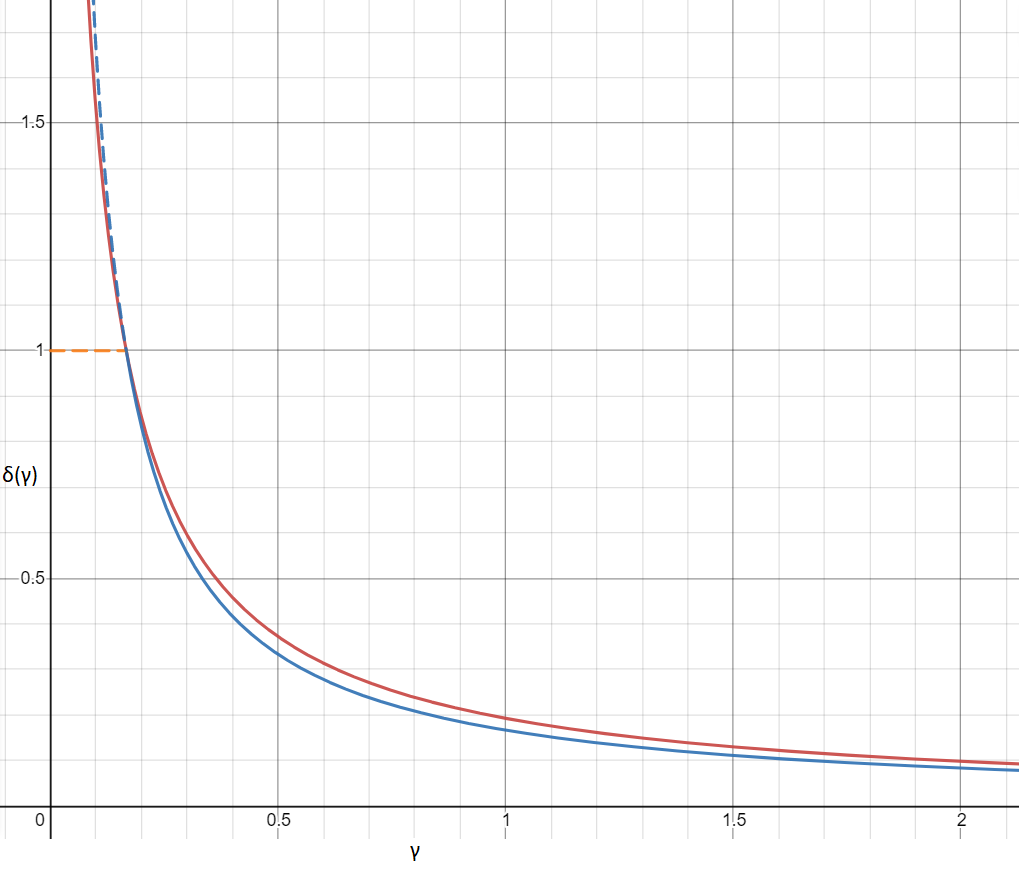
\includegraphics[width=340pt]{\resourceDir/img/Analysis/upper_bound_and_simplified_version.png}
				\end{figure}
				%\clearpage
				
				The red line is the inverse of the function ${ \delta^2 + 5\delta }$ (for positive values) that we have established as an upper bound on the value of ${ \abs{(x^2 + x) - 6} }$ and the blue line is the inverse of $6\delta$ (so ${ \delta = \frac{\epsilon}{6} = \frac{1}{6\gamma} }$).\\
				
				As we can see, for values of ${ \epsilon < 6 \iff \gamma > \frac{1}{6} }$, the blue line is underneath the red line which tells us that if we use those values for $\delta$ then we will definitely satisfy the limit condition. This can be seen more clearly in the below maginification of an area of the graph.\\
				\begin{figure}[h!]
					\centering
					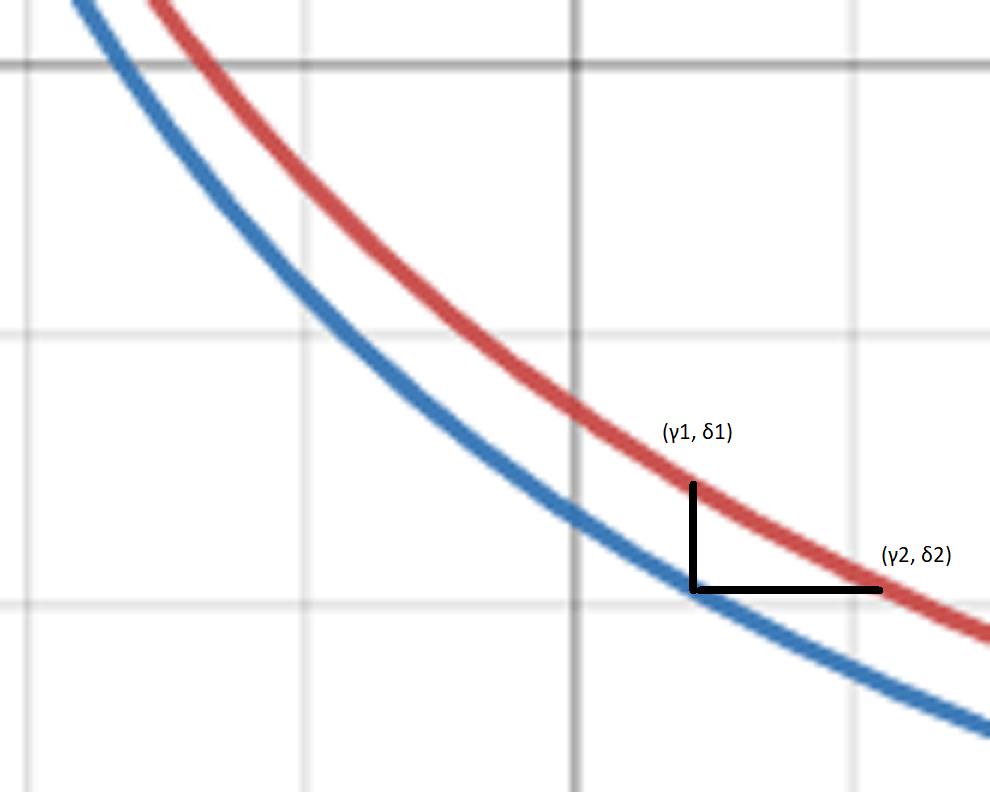
\includegraphics[width=340pt]{\resourceDir/img/Analysis/upper_bound_and_simplified_version_blow_up.png}
				\end{figure}
				
				By using the function represented by the blue line, for the value ${ \gamma = \gamma_1 }$ (which corresponds to some value of $\epsilon$) we return --- instead of $\delta_1$ --- the value $\delta_2$ with ${ \delta_2 < \delta_1 }$. The red line tells us that $\delta_2$ actually suffices for a bound ${ \gamma_2 > \gamma_1 }$. We therefore have
				\[ \abs{x - 2} < \delta_2 \implies \abs{(x^2 + x) - 6} < \frac{1}{\gamma_2} < \frac{1}{\gamma_1} \]
				which shows that the blue line gives a tighter bound than necessary and so is also valid. Referring back to the main graph, we can see that the blue dotted line shows that the blue line crosses the red line at ${ \epsilon = 6 \iff \gamma = \frac{1}{6} }$ and so is no longer valid for achieving the required $\epsilon$-neighbourhood.\\
				
				However, instead, we can use the orange dotted line as values of $\delta$ for the remaining values of $\gamma$. This corresponds to the following function,
				\[\begin{aligned}
					\delta(\epsilon) &= 	\begin{cases}
												\frac{\epsilon}{6} & \epsilon \leq 6 \\
												1 & \epsilon > 6
											\end{cases} \nn
					&= \min \left\{ \frac{\epsilon}{6}, 1 \right\}.
				\end{aligned}\]
			
				If we use this function to define the $\delta$ for any $\epsilon$ then, since \textit{both} 1 and ${ \frac{\epsilon}{6} }$ are an upper bound on the value of $\delta$ (which means that even if $\epsilon$ is arbitrarily large, $\delta$ is still upper-bounded by 1), we can therefore reason that,
				\[ \abs{(x^2 + x) - 6} < \delta (\delta + 5) \leq 6 \delta \leq 6 \frac{\epsilon}{6} = \epsilon. \]
			}
		\end{exe}
	}




% -------------------
\pagebreak
	
	
	
	\subsubsection{Continuity}
	{\tiny 
		\hyperref[ssssection:continuity-over-sequences]{continuity over sequences} \hspace{20pt} \hyperref[ssssection:continuity-on-closed-intervals]{continuity-on-closed-intervals}\\
	}

	\boxeddefinition{\textbf{(Continuity at a point)} 
		A function $ f $ is \textit{continuous at a point $a$} if
		\begin{itemize}
			\item{$f(a)$ is defined,}
			\item{${ \lim_{x \to a} f(x) = f(a) }$.}
		\end{itemize}
		\smallskip
		More formally, the definition of ${ \lim_{x \to a} f(x) = L }$ is,
		\[ \forall \epsilon > 0 \logicsep \exists \delta \suchthat 0 < \abs{x - a} < \delta \implies \abs{f(x) - L} < \epsilon. \]
		But if $f(a)$ is defined, then when ${ \abs{x - a} = 0 }$ (i.e. when ${ x = a }$) we have 
		\[ f(x) = f(a) \implies \abs{f(x) - f(a)} = 0 < \epsilon. \]
		Therefore, if $f(a)$ is defined and ${ \lim_{x \to a} f(x) = f(a) }$, then
		\[ \forall \epsilon > 0 \logicsep \exists \delta > 0 \suchthat \abs{x - a} < \delta \implies \abs{f(x) - f(a)} < \epsilon. \]		
	\label{def:continuity}}
	
	\boxeddefinition{\textbf{(Continuous Function)} A function is \textit{continuous} if it is \textit{continuous at every point in its domain}.}
	
	\boxeddefinition{\textbf{(Continuity on a closed interval)} A function is \textit{continuous on the closed interval $[a, b]$} if it is
		\begin{itemize}
			\item{continuous at every point in the open interval ${ (a, b) }$,}
			\item{${ \lim_{x \to a^+} f(x) = f(a) }$,}
			\item{${ \lim_{x \to b^-} f(x) = f(b) }$.}
		\end{itemize}
	}

	\boxeddefinition{\textbf{(Left and Right-Continuity)} A function is \textit{left continuous} or \textit{continuous on the left} at $a$ if,
		\[ \lim_{x \to a-} f(x) = f(a). \]
		Obviously, from the other side, a function can be \textit{right continuous}.
	}

	\labeledProposition{Let ${ f,g : \R{} \to \R{} }$ be functions that are continuous at ${ a \in \R{} }$ and $ c $ be
		any real number. Then ${ \abs{f}, (cf), (f - g), (f + g), (f(x)g(x)) }$ are all continuous at $ a $, and
		${ (f/g)  }$ is continuous provided ${ g(x) \neq 0 }$ for any $ x $ in some neighbourhood of $ a $.}{}
	\begin{proof}
		This follows from the algebra of finite limits of functions given in \autoref{prop:func-finite-limit-algebra}.
	\end{proof}

	\begin{corollary}
		It follows then that every polynomial is continuous. This can be seen as the most simple polynomial is a constant - which is clearly continuous; also ${ f(x) = x }$ is clearly continuous. Then powers of $x$ are continuous as they are products of continuous functions and when multiplied by coefficients this is a constant multiplying a continuous function so the resultant function is continuous. Then any polynomial is a summation of such terms so the result is continuous as the sum of continuous functions is continuous.
	\end{corollary}

	\labeledProposition{If $ g $ is a function which is continuous at $ a $, and $ f $ is a function which is
		continuous at $ g(a) $. Then ${ (f \circ g)  }$ is continuous at $ a $.}{composition-of-continuous-funcs-is-continuous}
	\begin{proof}
		Continuity of $f$ at $g(a)$ guarantees that for any ${ \epsilon > 0 }$ there exists some ${ \delta' > 0 }$ such that ${ \abs{x' - g(a)} < \delta' \implies \abs{f(x') - f(g(a))} < \epsilon }$ and continuity of $g$ at $a$ guarantees that for any ${ \delta' > 0 }$ there exists some ${ \delta > 0 }$ such that ${ \abs{x - a} < \delta \implies \abs{g(x) - g(a)} = \abs{x' - g(a)} < \delta' }$.
	\end{proof}
	\begin{corollary}
		If $ g $ is a function which is continuous at $ a $, and $ f $ is a function which is
		continuous at $ g(a) $. Then,
		\[ \lim_{x \to a} (f \circ g)(x) = \lim_{x \to a} f(g(x)) = f(\lim_{x \to a} g(x)). \]
	\end{corollary}

	\nl[12]
	\subsubsubsection{Continuity over sequences}\label{ssssection:continuity-over-sequences}
	\nl[4]
	The following proposition gives an alternative definition of continuity over convergent sequences rather than explicit subsets of $\R{}$. An important point to note is that this proposition applies to "each sequence" with the described limit. This is important as it is possible to find an individual sequence such that the inference is not valid.\\
	
	For example, the constant sequence ${ \forall n \in \N{} \logicsep x_n = a }$ clearly tends to $a$ as ${ n \to \infty }$ but this would not imply continuity of $f$ as the limit of $f(x_n)$ for such a sequence would amount to saying that ${ f(a) = f(a) }$; in actual fact it doesn't say anything about the limit of $f$ at $a$ because the definition of the limit of a function doesn't depend on the behaviour at the point (\ref{def:continuity}). The definition of continuity is assertion of the equality of the limit of $f$ over values in the neighbourhood of $a$ (but not at $a$ itself) with the value of $f$ at $a$. So, continuity is implied by the fact that the limit of $f(x_n)$ for the constant sequence $x_n = a$ is equal to the limit of $f(x_n)$ for all other sequences $x_n$ whose limit is $a$.\\
	
	Another way of looking at it is that $f$ is continuous at $a$ because the limit there equals $f(a)$ however the argument converges to $a$.\\
	
	Refer to example \ref{ex:limit-at-a-point-requires-the-function-to-converge-to-the-same-value-over-every-sequence-converging-to-the-point}.
	
	\bigskip	
	\labeledProposition{A function $ f $ is continuous at $a$ if and only if for each sequence $(x_n)$ such that ${ \lim_{n \to \infty} x_n = a  }$ we have ${ \lim_{n \to \infty} f(x_n) = f(a) }$.}{continuity-of-functions-over-sequences}
	\begin{proof}
		Suppose that for each sequence $(x_n)$ such that ${ \lim_{n \to \infty} x_n = a  }$ we have ${ \lim_{n \to \infty} f(x_n) = f(a) }$. Then, for any ${ \epsilon > 0 \in \R{} }$ there exists some $N$ such that for all ${ n > N \in \N{} }$,
		\[ \abs{f(x_n) - f(a)} < \epsilon \]
		and also,
		\[ \abs{x_n - a} < \delta \]
		for some ${ \delta > 0 \in \R{} }$. Since this applies to all such sequences it follows that
		\[ \abs{x - a} < \delta \; \implies \; \abs{f(x) - f(a)} < \epsilon \]
		and so ${ \lim_{x \to a} f(x) = f(a) }$ and $f$ is continuous at $a$.\\
		
		Conversely, suppose that $f$ is not continuous at $a$. Then
		\[\begin{aligned}
			&& \lnot ( \forall \epsilon > 0 \in \R{} \logicsep \exists \delta \logicsep \abs{x - a} < \delta \implies \abs{f(x) - f(a)} < \epsilon ) \\
			&\iff & \exists \epsilon > 0 \in \R{} \logicsep \lnot ( \exists \delta \logicsep \abs{x - a} < \delta \implies \abs{f(x) - f(a)} < \epsilon ) \\
			&\iff & \exists \epsilon > 0 \in \R{} \logicsep \forall \delta \logicsep \lnot ( \abs{x - a} < \delta \implies \abs{f(x) - f(a)} < \epsilon ) \\
			&\iff & \exists \epsilon > 0 \in \R{} \logicsep \forall \delta \logicsep \exists x \logicsep \abs{x - a} < \delta \; \land \; \abs{f(x) - f(a)} \geq \epsilon.
		\end{aligned}\]
		So, there exists a value of $\epsilon$ such that, for all ${ \delta > 0 }$, there is some $x$ in the $\delta$-neighbourhood of $a$ with ${ \abs{f(x) - f(a)} \geq \epsilon }$ and we can construct a sequence of such $x$-values in $\delta$-neighbourhoods with decreasing $\delta$ by establishing a relationship between the sequence index $n$ and $\delta$ such that $\delta$ decreases with increasing $n$. The simplest such relationship is
		\[ \delta = 1/n. \]
		Then $(x_n)$ is a sequence such that each term $x_n$ is an $x$-value in the $\delta$-neighbourhood of $a$ with ${ \abs{f(x) - f(a)} \geq \epsilon }$ and, since $\delta$ is decreasing with increasing $n$ we have ${ \lim_{n \to \infty} x_n = a }$ but there is no $N$ such that, for all ${ n > N }$, ${ \abs{f(x) - f(a)} < \epsilon }$. Therefore ${ \lim_{n \to \infty} f(x_n) \neq f(a) }$.
	\end{proof}
	\smallskip
	\begin{corollary}\label{cor:lim_of_func_of_convergent_sequence_is_func_of_limit}
		For a function $f$ that is continuous at $a$, 
		\[ \lim_{n \to \infty} f(x_n) = f\left( \lim_{n \to \infty} x_n \right). \]
	\end{corollary}
	\begin{proof}
		This is just a rewriting of \autoref{prop:continuity-of-functions-over-sequences}.
	\end{proof}

	
	
	\sep
	\begin{exe}
		\ex{
			The indicator function for rational numbers within the reals, known as the \textbf{Dirichlet Function},
			\[ 
			f(x) =	\begin{cases} 
			0 & x \text{ is irrational} \\
			1 & x \text{ is rational}
			\end{cases}. 
			\]
			This function is nowhere continuous because between every two irrational numbers there is a rational number (and vice-versa) so $f(x)$ is flipping between 0 and 1 in every neighbourhood of every point however small a neighbourhood we consider. So this function never converges anywhere but \textit{is} bounded because it only ever takes values of 1 or 0 so, clearly, its maximum is 1 and minimum is 0.
		}\label{ex:dirichlet_function}
		\bigskip
		\ex{
			The function ${ f(x) = 1/x }$ over the interval ${ (0,1] }$ is continuous at every point but unbounded as it goes to infinity as ${ x \to 0 }$. If we consider the same function over the closed interval ${ [0,1] }$ then we no longer have continuity over this interval as there is a singularity at ${ x = 0 }$.\\
			
			However, if we define the function at ${ x = 0 }$ so that we have a new function,
			\[
				g(x) =
				\begin{cases}
					1/x & x \neq 0 \\
					1 & x = 0
				\end{cases} 
			\]
			then the function $g$ is unbounded on the closed interval ${ [0,1] }$ despite also being defined at every point in the interval. The reason is that we have removed the singularity at 0 by defining a finite value at the point. This creates a jump-discontinuity at 0 so we have sacrificed continuity in order to achieve this.
		}\label{ex:reciprocal_function}
	\end{exe}
	
	
	
	
	\nl[16]
	\subsubsubsection{Continuity on Closed Intervals}\label{ssssection:continuity-on-closed-intervals}
	\nl[6]
	\boxeddefinition{\textbf{(Closed Interval)} A \textit{closed} interval is an interval in which every convergent sequence of values in the interval, converges to a point in the interval.
	\label{def:closed-interval}}

	\paragraph{The Extreme Value Theorem} shows that if a function is continuous on a closed interval then it follows that the function is bounded and attains both its maximum and minimum (i.e. its supremum is a maximum and its infimum is a minimum) on the interval.
	\note{Note that, even if $f$ is defined at every point in ${ [a,b] }$, if it is not continuous then it \textit{may} not be bounded. There \textit{do} exist functions that are not continuous but bounded (for example the Dirichlet Function \ref{ex:dirichlet_function}) but there also exist functions that are not continuous and unbounded such as the reciprocal function (\ref{ex:reciprocal_function}). So, functions that are not continuous on a closed interval may be bounded or not; and functions that are continuous on an open interval also may or may not be bounded (again, the reciprocal function is an example of a function that is continuous on an open interval but not bounded); but here we will show that functions that are continuous on a closed interval must be bounded on that interval and then it will also follow that the maximum and minimum is attained.
	}

	\bigskip
	\begin{lemma}\label{lem:continuity-on-closed-interval-implies-boundedness}
		Let $f: \R{} \longmapsto \R{} $ be continous on ${ [a,b] }$. Then $f$ is bounded on ${ [a,b] }$.
	\end{lemma}
	\begin{proof}
		Assume for contradiction, that $f$ is unbounded above on the interval. Then for any ${ M \in \R{} }$, there is some ${ x \in [a,b] }$ such that ${ f(x) > M }$. So there is a sequence $(x_n)$ such that, for all ${ n \in \N{} }$,
		\[ x_n \in [a,b] \; \land \; f(x_n) > n. \]
		But $(x_n)$ is a bounded sequence and so, by Bolzano-Weierstrass (\autoref{theo:every_bounded_seq_has_convergent_subseq}), has a convergent subsequence $(x_{k_n})$ which must converge to some point in the interval, say $c$. But then continuity of $f$ on the interval and \autoref{prop:continuity-of-functions-over-sequences} imply that ${ \lim_{k_n \to \infty} f(x_{k_n}) = f(c) }$ but
		\[ f(x_{k_n}) > k_n \; \implies \; f(x_{k_n}) \to \infty \eqword{as} k_n \to \infty. \]
		Therefore $f$ is bounded above.\\
		By a similar argument we can show that $f$ must also be bounded below.
	\end{proof}

	\bigskip
	\begin{lemma}\label{lem:continuity-and-boundedness-on-closed-interval-implies-supremum-is-max-and-infimum-is-min}
		Let $f: \R{} \longmapsto \R{} $ be continous and bounded on ${ [a,b] \subset \R{} }$. Then $f$ attains its maximum and minimum on ${ [a,b] }$.
	\end{lemma}
	\begin{proof}
		Since $f$ is bounded on ${ [a,b] }$, the set ${ S = \setc{ f(x) \in \R{} }{ x \in [a,b] } }$ is bounded. Then, by \autoref{axiom:continuum-property}, $S$ has a supremum and an infimum. Let ${ \sigma = \sup S }$. Then, by the definition of the supremum (\ref{def:supremum}),
		\[ \forall \epsilon > 0 \in \R{} \logicsep \exists s \in S \logicsep s + \epsilon > \sigma \iff \sigma - s < \epsilon. \]
		Therefore, if we let ${ \epsilon = 1/n }$, then there is a sequence $(x_n)$ such that, for all ${ n \in \N{} }$,
		\[ x_n \in [a,b] \; \land \; \sigma - f(x_n) < \epsilon = 1/n \]
		where, because $\sigma$ is an upper bound on $f(x_n)$ we have 
		\[ \sigma - f(x_n) = \abs{\sigma - f(x_n)} < \epsilon. \]
		So, clearly, for any value of $\epsilon$, there exists an ${ N = 1/\epsilon }$ such that,
		\[ \forall n > N \in \N{} \logicsep \abs{\sigma - f(x_n)} < \epsilon \]
		and ${ \lim_{n \to \infty} f(x_n) = \sigma }$.\\
		
		Furthermore, since the sequence $(x_n)$ is bounded in the interval $[a,b]$, by Bolzano-Weierstrass (\autoref{theo:every_bounded_seq_has_convergent_subseq}), it has a convergent subsequence $(x_{k_n})$ which must converge to some point in the interval, say $c$. But then continuity of $f$ on the interval and \autoref{prop:continuity-of-functions-over-sequences} imply that
		\[ f\left( \lim_{k_n \to \infty} x_{k_n} \right) = f(c) = \sigma. \]
		
		Therefore, $f$ attains its supremum. By a similar argument we can show that $f$ also attains its infimum.
	\end{proof}

	\bigskip
	\labeledTheorem{\textbf{(Extreme Value Theorem)} If a real-valued function $f$ is continous on the closed interval ${ [a,b] }$ then it attains a maximum and minimum on the interval.}{extreme-value-theorem}
	\begin{proof}
		By \autoref{lem:continuity-on-closed-interval-implies-boundedness}, $f$ is bounded on the interval and then, by \autoref{lem:continuity-and-boundedness-on-closed-interval-implies-supremum-is-max-and-infimum-is-min}, $f$ attains a maximum and minimum.
	\end{proof}

	\bigskip
	\note{This proof of Extreme Value Theorem says: Assume that $f$ is unbounded on the interval. Then we can construct a sequence of $x$-values such that, for the $n$th value $x_n$, ${ f(x_n) > n }$. This is possible because, if $f$ is unbounded, for any value of $n$, there is some subinterval of $x$-values such that for each of them ${ f(x) > n }$ and any interval of the real numbers contains an infinite number of real numbers and so, a sequence $x_n$ with ${ n \to \infty }$. Note that, at this point, $x_n$ is an arbitrary sequence which is not necessarily convergent (it could bounce around the interval).\\
		Then, we notice that this sequence $x_n$ is necessarily bounded (as it is a subinterval of ${ [a,b] }$) and so we invoke the Bolzano-Weierstrass Theorem, \autoref{theo:every_bounded_seq_has_convergent_subseq} (called Theorem 10.11 in the quoted proof), to deduce that it has a convergent subsequence which we call $x_{k_n}$ and call its limit $c$.\\
		At this point we can use the continuity of $f$ on the interval to deduce that ${ f(x_{k_n}) \to f(c) }$ as ${ n \to \infty }$ by which we obtain a contradiction to the condition we set on the values of $x_{k_n}$ when we constructed the sequence -- namely that ${ f(x_{k_n}) > n }$. Notice that this is constructing a sequence $x_{k_n}$ such that $f(x_{k_n})$ grows without bound as ${ n \to \infty }$ and then saying, "but the limit of $x_{k_n}$ as ${ n \to \infty }$ is $c$ which is inside the interval and so (by continuity) the limit of $f(x_{k_n})$ as ${ n \to \infty }$ is $f(c)$ -- a fixed finite value". This is the point where the fact that the interval ${ [a,b] }$ is closed comes into play -- if the interval were not closed it would be possible that $c$ was not inside the interval and then we would not be able to invoke continuity to assert that the limit of $f(x_{k_n})$ over this sequence was finite.\\
		So, now we have shown that if a function is continuous over a closed interval then assuming that the function is unbounded produces a contradiction and, therefore, we can conclude that it is, in fact, bounded.\\
		The last thing that needs to be proven is that $f$ obtains its maximum in the interval. Having shown that the function is bounded on the interval we now know that there exists
		\[ M = \text{sup}\setc{f(x)}{x \in [a, b]} \]
		and we need to show that there is such an $x$-value in ${ [a,b] }$ that ${ f(x) = M }$. In an open interval this might not be the case as the supremum of the function on the interval might occur as the limit of $f$ over a sequence of $x$-values converging to a point that lies outside the interval. So, in this case, we construct a convergent sequence such that ${ f(x_{k_n}) \to M }$ as ${ n \to \infty }$ by selecting $x_n$ such that ${ f(x_n) = M - \frac{1}{n} }$. This is possible because the definition of the supremum says that, because it is the \textit{lowest} upper bound,
		\[ \forall \epsilon > 0 \logicsep \exists f(x_n) \logicsep f(x_n) > M - \epsilon \]
		and so we are letting ${ \epsilon = \frac{1}{n} }$. Then, as previously, we take a convergent subsequence of this sequence and name it $x_{k_n}$. So, as before, we have a sequence converging on some point, we'll call it ${ c \in [a,b] }$, at which $f$ is continuous so that ${ f(x_{k_n}) \to M }$ as ${ n \to \infty }$ implies that ${ M = f(c) }$. This, in turn, means that $f$ obtains a maximum in the interval.
	}
	


	\bigskip
	\paragraph{The Intermediate Value Theorem} says that if a function is continuous on a closed interval and takes different value at the bounds of the function, then it must also attain any value in between the values that it attains at the bounds of the interval.\\
	Note that this theorem is \textit{not} written for an interval such that ${ f(a) \leq f(b) }$ because if ${ f(a) = f(b) }$ then the only ${ K \suchthat f(a) \leq K \leq f(b) }$ is ${ f(a) = K = f(b) }$. But now it is \textit{not} true to say that there exists some ${ c \in (a,b) }$ with ${ f(c) = K }$ as there is no reason why the value of $f(x)$ at the bounds of the interval should be repeated somewhere in the interior of the interval.
	
	\bigskip
	\labeledTheorem{\textbf{(Intermediate Value Theorem)} Let $f$ be continuous on ${ [a,b] }$ with ${ f(a) < f(b) }$. Then, for all ${ K \suchthat f(a) < K < f(b) }$, there exists some ${ c \in (a,b) }$ with ${ f(c) = K }$.
	}{intermediate_value_theorem}
	\note{\question{What is wrong with the following proof?}
		\begin{proof}Suppose ${ \centernot\exists x \in [a,b] \suchthat f(a) < f(x) < f(b) }$. Since we know that at ${ x = a }$ the value is $f(a)$ and at ${ x = b }$ the value is $f(b)$ with ${ f(b) > f(a) }$, we can deduce that,
		\[ \exists c \in [a,b] \suchthat \lim_{x \to c^-} f(x) = f(a) \land \lim_{x \to c^+} f(x) = f(b). \]
		But this contradicts the hypothesis that $f$ is continuous on the entire interval. Therefore, there must exist some
		\[ x \in [a,b] \suchthat f(a) < f(x) < f(b). \]
		But then we can recursively apply this same logic to the intervals ${ [f(a),f(x)] }$ and ${ [f(x),f(b)] }$ to show that there must be values of $f$ between them also. Since it is always possible for us to apply the reasoning to any interval however small, we can conclude that between any distinct values of the function ${ f(x_1) < f(x_2) }$, there must be an intermediate value of the function ${ f(x_1) < f(x_3) < f(x_2) }$. $\qedhere$	
		\end{proof}
	}
	\medskip
	We begin by proving a special case from which the general proof will follow.
	\begin{lemma}
		Let $f$ be continuous on ${ [a,b] }$ with ${ f(a) < 0 < f(b) }$. Then there exists some ${ c \in (a,b) }$ with ${ f(c) = 0 }$.
	\end{lemma}
	\begin{proof}
		We construct a sequence of intervals ${ [a_n, b_n] }$ such that
		\begin{enumerate}
			\item{${ f(a_n) < 0,\; f(b_n) > 0 }$ for each $ n $}
			\item{${ [a_{n+1}, b_{n+1}] \subseteq [a_n, b_n] }$ for each $ n $.}
		\end{enumerate}				
		We start by letting ${ [a_1, b_1] = [a, b]. }$ Then for each ${ n \geq 1 }$, we define ${ [a_{n+1}, b_{n+1}] }$ as follows.\\
		
		Let ${ c_n = (a_n + b_n)/2 }$, be the midpoint of the previous interval. If ${ f(c_n) = 0, }$ then the
		theorem is proved and so we need not continue constructing intervals!\\
		
		Otherwise, if ${ f(c_n) < 0 }$, we define ${ a_{n+1} = c_n }$ and ${ b_{n+1} = b_n }$. And if ${ f(c_n) > 0 }$, we define
		${ b_{n+1} = c_n }$ and ${ a_{n+1} = a_n }$. Note that the condition 1. is satisfied by choosing our intervals in this manner.
		Moreover, note that the ${ (n + 1) }$st interval is half the size of the $n$th interval and so
		${ b_{n+1} - a_{n+1} \leq (b_1 - a_1)/2^n }$. It follows that
		\[ \lim_{n \to \infty} (b_n - a_n) = 0.  \tag{*}\]
		
		Finally, note that $(a_n)$ is increasing and bounded above (by $b_1$) and so it has a limit; similarly $(b_n)$ is decreasing and bounded below and so has a limit. Thus by (*), and algebra of finite limits (\autoref{prop:func-finite-limit-algebra}), these limits are equal to, say, $c$. Thus by continuity (using \autoref{prop:continuity-of-functions-over-sequences}),
		\[ f(c) = \lim_{n \to \infty} f(b_n) \geq 0, \]
		where the last inequality follows from the fact that each ${ f(b_n) \geq 0 }$ (in fact > 0). 
		\note{Note that ${ f(b_n) > 0 }$ so the limit of $f(b_n)$ is ${ \geq 0 }$.}
		Similarly,
		\[ f(c) = \lim_{n \to \infty} f(a_n) \leq 0. \]
		Thus $ f(c) $ must be equal to zero, and the proof is complete.
	\end{proof}
	Clearly, the general proof of the Intermediate Value Theorem follows naturally from this because,
	\begin{itemize}
		\item{If ${ f(a) > f(b) }$ then we can consider the function ${ g(x) = -f(x) }$ so that we have ${ g(a) < g(b) }$,}
		\item{If we have ${ K \suchthat f(a) < K < f(b) }$ with ${ K \neq 0 }$ we can consider ${ g(x) = f(x) - K }$ so that we have ${ g(a) < 0 < g(b) }$.}
	\end{itemize}
	So, the general problem posed in the Intermediate Value Theorem is reducible to the case we have proved.
	
	\bigskip
	\begin{corollary}
		\label{coro:continuous_func_mapping_interval_to_itself_has_invariant_point}
		Suppose that the real function $f$ is continuous on the closed interval ${ [a,b] }$ and that $f$ maps ${ [a,b] }$ into ${ [a,b] }$. Then there is ${ c \in [a,b] }$ with ${ f(c) = c }$.
	\end{corollary}
	\begin{proof}
		Let ${ h(x) = f(x) - x }$ so that ${ f(c) = c }$ if and only if ${ h(c) = 0 }$. Then also we have,
		\[ a \leq f(x) \leq b \implies h(a) \geq 0,\; h(b) \leq 0. \]
		If either of $h(a)$ or $h(b)$ is equal to 0 then we have found our $c$ such that ${ f(c) = c }$. Otherwise, if neither is equal to 0, then we must have ${ h(a) > 0 }$ and ${ h(b) < 0 }$. So, we may apply the Intermediate Value Theorem to conclude that there exists ${ c \in (a,b) }$ such that ${ h(c) = 0 }$ which is to say ${ f(c) = c }$.
	\end{proof}



	\sep
	\begin{exe}
		\ex{\textit{Suppose the real function $f$ is continuous, positive and unbounded on $\R{}$ and that ${ \inf \setc{f(x)}{x \in \R{}} = 0 }$. Use the Intermediate Value Theorem to prove that the range of $f$ is ${ (0,\infty) }$. }\\\\
			Let ${ y \in (0,\infty) }$. We show that there is some ${ c \in \R{} }$ such that ${ f(c) = y }$. This shows that the range is the whole of ${ (0,\infty) }$. (The fact that it is no larger follows from the given fact that $ f $ is positive.)\\
			Now,  ${ \text{inf}\,f(\R{}) = \text{inf}\,\setc{f(x)}{x \in \R{}} = 0 }$, so, since ${ y > 0 }$, there must be some ${ y_1 \in f(\R{}) }$ with ${ y_1 < y }$. This means there is some ${ x_1 \in \R{} }$ such that ${ y_1 = f(x_1) < y }$.\\
			Similarly, because $ f $ is unbounded, which means $ f(\R{}) $ is unbounded, there must be some ${ y_2 \in f(\R{}) }$ with ${ y_2 > y }$ and there will be some ${ x_2 \in \R{} }$ such that ${ y_2 = f(x_2) > y }$.\\
			Then $ y $ lies between $ f(x_1) $ and $ f(x_2) $ and, since $ f $ is continuous, the Intermediate Value Theorem shows that there is some $ c $ between $ x_1 $ and $ x_2 $ with ${ f(c) = y }$.
		}
	
		\bigskip
		\ex{\textit{Suppose the real function $g$ is continuous on $\R{}$ and that $g$ maps ${ [a,b] }$ into ${ [d,e] }$ and maps ${ [d,e] }$ into ${ [a,b] }$ where ${ a < b,\; d < e }$. By considering the function
					\[ k(x) = g(g(x)), \]
			prove that there are ${ p,q \in \R{} }$ such that
				\[ g(p) = q,\; g(q) = p. \]
			Hence show that there is ${ c \in \R{} }$ such that ${ g(c) = c }$.
			}\\\\
			The function $k$, being a composition of continuous functions, is continuous and also maps ${ [a,b] }$ into ${ [a,b] }$ so that we can use \autoref{coro:continuous_func_mapping_interval_to_itself_has_invariant_point} to deduce that there exists ${ c \in [a,b] }$ such that ${ k(c) = c }$. If we let ${ p = c }$ and ${ q = g(p) }$ then we have,
			\[ k(p) = p \iff g(g(p)) = p \iff g(q) = p. \]
			Now we can employ the same trick again by defining
			\[ h(x) = g(x) - x \]
			and then we have
			\[ h(p) = g(p) - p = q - p, \; h(q) = g(q) - q = p - q \]
			so that ${ h(p) = -h(q) }$ and therefore, either:
			\begin{itemize}
				\item ${ h(p) = 0 = h(q) }$, in which case ${ p = c = q }$ such that ${ g(c) = c }$; or else
				\item ${ h(x) }$ changes sign between $p$ and $q$. (Note that we don't know which of $p$ and $q$ is the lower end and upper end of the interval but we know that between the two values the function changes sign.) Then, applying the Intermediate Value Theorem we have some $c$ between $p$ and $q$ such that,
				\[ h(c) = 0 \iff g(c) - c = 0 \iff g(c) = c. \]
			\end{itemize}
			
		}
	\end{exe}
	

	
	\nl[18]
	\subsubsection{Functions in $\R{m}$}
	\bigskip
	\labeledProposition{Let ${ f: \R{n} \longmapsto \R{m} }$ and ${ f_1,f_2,\dots,f_m: \R{n} \longmapsto \R{} }$ such that
		\[ \forall \x \in \R{n} \logicsep f(\x) = (f_1(\x), f_2(\x), \dots, f_m(\x))^T. \]
		Then $f$ is continuous at ${ \y \in \R{n} }$ iff every $f_i$ for ${ 1 \leq i \leq m }$ is continuous at $\y$.
	}{vector-valued-function-is-continuous-iff-each-component-function-is-continuous}
	\begin{proof}
		This is a direct consequence of \autoref{prop:seq-in-Rm-converges-iff-every-component-converges-to-same-point}.
	\end{proof}

	\bigskip
	\labeledProposition{All linear functions are continuous.}{all-linear-functions-are-continuous}
	\begin{proof}
		Let ${ f: \R{n} \longmapsto \R{m} }$ be a linear function. Then, by \autoref{prop:every-lin-transform-is-left-multiplication-by-a-particular-matrix}, $f$ can be represented as left multiplication by a ${ m \times n }$ matrix. Let ${ A \in \R{m \times n} }$ be such that, for all ${ \x \in \R{n} }$,
		\[ f(\x) = A \x. \]
		Then, by \autoref{prop:vector-valued-function-is-continuous-iff-each-component-function-is-continuous}, $f$ will be continuous at ${ \a \in \R{n} }$ if, for each $i$ such that ${ 1 \leq i \leq m }$,
		\[ f_i(\x) = \inner{\e{i}}{A\x} = \e{i}^T A \x \]
		is continuous at $\a$.\\
		Assume we have $\x$ in some $\delta$-neighbourhood of $\a$ so that ${ \norm{\x - \a} < \delta }$. For any $i$,
		\[\begin{aligned}
			\norm{f_i(\x) - f_i(\a)} &= \norm{\e{i}^T A \x - \e{i}^T A \a} \nn
			&= \norm{\e{i}^T A (\x - \a)}  &\sidecomment{} \nn
			&\leq \norm{\e{i}^T A} \norm{\x - \a}  &\sidecomment{by cauchy-schwartz (\autoref{theo:cauchy-schwarz-inequality})} \nn
			&\leq \delta \norm{\e{i}^T A}.  &\sidecomment{equality case is if 0}
		\end{aligned}\]
		Since $\norm{\e{i}^T A}$ is the norm of the first row of $A$, it is just some non-negative constant real number, say $k$. Assume $k$ is non-zero. So, the result that
		\[ \norm{\x - \a} < \delta \; \implies \; \norm{f_i(\x) - f_i(\a)} < \delta k \]
		means that for any ${ \epsilon = \delta k }$ there is a $\delta$-neighbourhood around $\a$ such that, for any $\x$ in the neighbourhood, $f_i(\x)$ is in the $\epsilon$-neighbourhood of $f_i(\a)$. Therefore $f_i$ is continuous.\\
		Consider the case where ${ k = 0 }$: In this case the function $f_i$ is identically 0 and so, as a constant function, is trivially continuous.\\
		It follows then that, in all cases, $f$ is continuous.
	\end{proof}


	\nl[12]
	\sep
	\begin{exe}
		\ex Let ${ f,g: \R{2} \setminus \{ (0,0)^T \} \longmapsto \R{} }$ and let $f$ be given by,
		\[ f\begin{pmatrix}x_1\\x_2\end{pmatrix} = \frac{{x_2}^2 - {x_1}^2}{{x_1}^2 + {x_2}^2} \]
		and $g$ be given by,
		\[ g\begin{pmatrix}x_1\\x_2\end{pmatrix} = \frac{x_1{x_2}^2}{{x_1}^2 + {x_2}^4}. \]
		
		Let's examine the behaviour of the functions as ${ \x \to \0 }$ along a straight line defined by
		\[ x_2 = \alpha x_1 \eqword{for constant} \alpha \in \R{}. \]
		So, for ${ t \in \R{} }$,
		\[ \x = t \begin{pmatrix}1\\ \alpha\end{pmatrix} \to \begin{pmatrix}0\\0\end{pmatrix} \eqword{as} t \to 0. \]
		
		Firstly, we find an expression for the function values along such a line (note that the functions are not linear so we do not have ${ f(t\v) = tf(\v) }$),
		\[ f\begin{pmatrix}t\\ \alpha t\end{pmatrix} = \frac{(\alpha t)^2 - t^2}{t^2 + (\alpha t)^2} = \frac{\alpha^2 - 1}{1 + \alpha^2}, \]
		\[ g\begin{pmatrix}t\\ \alpha t\end{pmatrix} = \frac{t(\alpha t)^2}{t^2 + (\alpha t)^4} = \frac{t\alpha^2}{1 + \alpha^4 t^2}. \]
		
		\nl[2]
		The expression for $f$ tells us that, as ${ \x \to \0 }$ along a straight line, the value of $f$ is constant at a value that depends on the value of the constant $\alpha$. So, for different lines corresponing to different values of $\alpha$, the value of $f$ is different. Therefore, since as ${ \x \to \0 }$ along different lines it has a different value, ${ \lim_{\x \to \0} f(\x) }$ \textit{does not exist}.\\
		
		On the other hand, the expression for $g$ tells us that, as ${ \x \to \0 }$ along a straight line, the value of $g$ goes to 0 regardless of the value of the constant $\alpha$. That's to say, along whichever straight line in $\R{2}$ we approach the origin, $g$ is going to 0. However, \textit{we cannot conclude that the limit of $g$ exists at $\0$} because this only covers the behaviour over straight lines. By \autoref{prop:continuity-of-functions-over-sequences} (\TODO{this proposition is about continuity; is it worth separating it into a proposition about limits of functions with a corollary about continuity?}), the limit of the function only exists at a point if the function converges to the same value along all sequences that converge to the point.\\
		
		In this case we can construct a sequence that follows a parabolic path towards the origin, ${ x_1 = \alpha {x_2}^2 }$, parametrically expressed as
		\[ \x = \begin{pmatrix}\alpha t^2\\ t\end{pmatrix} \to \begin{pmatrix}0\\0\end{pmatrix} \eqword{as} t \to 0. \]
		The expression for the value of $g$ along this parabola comes out as,
		\[ g\begin{pmatrix}\alpha t^2\\ t\end{pmatrix} = \frac{(\alpha t^2) t^2}{(\alpha t^2)^2 + t^4} = \frac{\alpha}{\alpha^2 + 1}. \]
		Therefore, for $g$, along parabolic lines of this form, the value of $g$ is a constant depending on the value of $\alpha$. So, once again, over different sequences (defined by different values of $\alpha$) approaching $\0$, the value of $g$ is converging to (actually staying constant at) different values. Once again then, the limit of $g$ \textit{does not exist} at $\0$.
		\label{ex:limit-at-a-point-requires-the-function-to-converge-to-the-same-value-over-every-sequence-converging-to-the-point}
	\end{exe}



% ----------- break ------------
\pagebreak
	
	
	
	\subsubsection{Relationship Between Sequences and Functions}\bigskip
	Let ${ f: \R{} \mapsto \R{},\; f(x) = y. }$ Now imagine that we take regular intervals on the domain, say, interval 1. We name the $x$-values at the upper bound of these intervals $x_1, x_2, \dots$ for $x = 1, 2, \dots$. Then, the corresponding $y$-values, $y = f(x_1), f(x_2), \dots$ can be named $y_1, y_2, \dots$. In this way, we have defined a sequence, ${ y_n = f(x_n) }$ where ${ x_n \in \N{} }$ (note that this is a different notation from that used before where a sequence ${ x_n = f(n) }$ for ${ n \in \N{} }$).\\
	Looking at the derivative of the function,
	\[ \frac{dy}{dx} \approxeq \frac{\Delta y}{\Delta x} = \frac{ f(x_{n+1}) - f(x_n) }{1} = f(x_{n+1}) - f(x_n). \]
	While the ratio of consecutive terms is,
	\[ \frac{y_{n+1}}{y_n} = \frac{y_n + \Delta y}{y_n} = \frac{f(x_{n+1})}{f(x_n)} =  \frac{f(x_n) + (f(x_{n+1}) - f(x_n))}{f(x_n)}. \]
	Note, also, that
	\[ \frac{y_n + \Delta y}{y_n} = 1 + \frac{\Delta y}{y_n} \approxeq 1 + \frac{dy/dx}{y} = 1 + \frac{d}{dx} \ln{y} \]
	which is to say that ${ \frac{\Delta y}{y_n} }$ is the discrete form of the log derivative.
	Clearly, when ${ \Delta y > 0 }$, we can put this in the form
	\[ \frac{y_{n+1}}{y_n} = 1 + \frac{\Delta y}{y_n} = 1 + \frac{ \Delta y/y_n }{1} = \frac{1 + h}{1}. \]
	If ${ \Delta y < 0 }$ however,
	\[ \frac{y_n + \Delta y}{y_n} = \frac{1}{y_n/(y_n + \Delta y)} = \frac{1}{\frac{y_n + \Delta y - \Delta y}{y_n + \Delta y}} = \frac{1}{1 + \frac{-\Delta y}{y_n + \Delta y}} = \frac{1}{1 + h}. \]
	If ${ \frac{\Delta y}{y_n} }$ does not go to 0 then the ratio of consecutive terms stays below 1 and the sequence converges to 0. If it does go to 0 then the ratio of consecutive terms goes to 1 and the sequence may converge to 0 or to some non-zero value. These cases appear (proof?) to be distinguishable by looking at how fast ${ \frac{\Delta y}{y_n} }$ goes to 0. For example,
	\begin{enumerate}[label=(\roman*)]
		
		\item{${\bm{ a_n = \frac{1}{n} + 1 }}$}
		\[ \lim_{n \to \infty} \frac{1}{n} + 1 = 1 \]
		\[ \frac{\Delta a}{a_n} = \frac{-1}{(n+1)^2} \]
		
		\item{${\bm{ a_n = \frac{1}{n} }}$}
		\[ \lim_{n \to \infty} \frac{1}{n} = 0 \]
		\[ \frac{\Delta a}{a_n} = \frac{-1}{n+1} \]
	\end{enumerate}
	Maybe the fact that ${ \frac{\Delta y}{y_n} }$ goes to 0 faster as ${ n \to \infty }$ in the first case indicates that it converges before it gets to 0?




% -------------- break ----------------
\pagebreak


	\searchableSubsection{Differentiation}{analysis, real analysis}{
		\bigskip
		\boxeddefinition{\textbf{(Differentiability)} A function $f$ over $\R{}$ is \textit{differentiable} over an interval ${ (a,b) \subset \R{} }$ iff, for all ${ y \in (a,b) }$, the limit
			\[ \lim_{x \to y} \frac{f(x) - f(y)}{x - y} \]
			exists. This implies, by the definition of the limit, that the left and right limits, denoted $f_r'$ and $f_l'$, \textit{both exist and are equal}.
		\label{def:differentiability}}
		
		
		\biggerskip
		\labeledProposition{Differentiability at a point $c$ implies continuity at $c$.}{differentiability-implies-continuity}
		\begin{proof}
			Differentiability at $c$, by definition (\ref{def:differentiability}), implies that
			\[ \lim_{x \to c} \frac{f(x) - f(c)}{x - c} = L \]
			for some finite ${ L \in \R{} }$. Since we also have,
			\[ \lim_{x \to c} (x - c) = 0 \]
			which, clearly, is a finite limit, we can use the algebra of finite limits (\autoref{prop:func-finite-limit-algebra}) to deduce that
			\[ \left( \lim_{x \to c} (x - c) \right) \left( \lim_{x \to c} \frac{f(x) - f(c)}{x - c} \right) = \lim_{x \to c} (f(x) - f(c)). \]
			Therefore,
			\[ 0 \times L = 0 = \lim_{x \to c} (f(x) - f(c)) \]
			and so ${ \lim_{x \to c} f(x) = f(c) }$ as is necessary for continuity. Then, we can also reason that $f(c)$ must be defined and finite for an expression involving it to be defined and finite, and so differentiability also implies that $f(c)$ is defined and finite.\\
			
			Therefore, $f$ is continuous at $c$.
		\end{proof}
	
		\bigskip
		\labeledProposition{\textbf{(Product and Quotient Rule)} Let $f,g$ be defined on ${ (a,b) }$ and differentiable at ${ c \in (a,b) }$. Then,
			\begin{enumerate}[label=(\roman*)]
				\item ${ (f + g)'(c) = f'(c) + g'(c) }$;
				\item ${ (fg)'(c) = f'(c)g(c) + f(c)g'(c) }$ where $fg$ denotes the pointwise product;
				\item if ${ g(c) \neq 0 }$ then ${ (f/g)'(c) = \frac{ f'(c)g(c) - f(c)g'(c) }{ g(c)^2 } }$.
			\end{enumerate}
		}{differentiation-product-and-quotient-rule}
		\begin{proof}\nl
			\begin{enumerate}[label=(\roman*)]
				\item Because $f'(c)$ and $g'(c)$ both exist the derivatives are finite and we can apply the algebra of finite limits (\autoref{prop:func-finite-limit-algebra}) so that,
				\[ \lim_{x \to c} \frac{f(x) + g(x) - f(c) - g(c)}{x - c} = \lim_{x \to c} \frac{f(x) - f(c)}{x - c} + \lim_{x \to c} \frac{g(x) - g(c)}{x - c}. \]
				
				\bigskip
				\item Since $f$ and $g$ are both differentiable on the interval, by \autoref{prop:differentiability-implies-continuity}, they are also both continuous. Therefore,
				\[\begin{aligned}
					&\lim_{x \to c} \frac{f(x)g(x) - f(c)g(c)}{x - c} \nnn
					&= \lim_{x \to c} \frac{f(x)g(x) - f(c)g(c) + f(x)g(c) - f(x)g(c)}{x - c} \nnn
					&= \lim_{x \to c} \frac{(f(x)g(c) - f(c)g(c)) + (f(x)g(x) - f(x)g(c))}{x - c} \nnn
					&= \lim_{x \to c} g(c)\frac{f(x) - f(c)}{x - c} + \lim_{x \to c} f(x)\frac{g(x) - g(c)}{x - c} &\sidecomment{by \autoref{prop:func-finite-limit-algebra}} \nnn
					&= f'(c)g(c) + f(c)g'(c).  &\sidecomment{by continuity}
				\end{aligned}\]
				
				\bigskip
				\item Using ${ g(c) \neq 0 }$ and the continuity of $f$ and $g$ at $c$,
				\[\begin{aligned}
					&\lim_{x \to c} \frac{f(x)/g(x) - f(c)/g(c)}{x - c} \nnn
					&= \lim_{x \to c} \frac{1}{x - c} \frac{f(x)g(c) - f(c)g(x)}{g(x)g(c)} \nnn
					&= \lim_{x \to c} \frac{1}{g(x)g(c)} \frac{ f(x)g(c) - f(c)g(x) + f(x)g(x) - f(x)g(x) }{ x - c } \nnn
					&= \lim_{x \to c} \frac{1}{g(x)g(c)} \frac{ (f(x)g(x) - f(c)g(x)) + (f(x)g(c) - f(x)g(x)) }{ x - c } \nnn
					&= \lim_{x \to c} \frac{1}{g(x)g(c)} \left( g(x)\frac{ f(x) - f(c) }{ x - c } - f(x)\frac{ g(x) - g(c) }{ x - c } \right) \nnn
					&= \frac{ f'(c)g(c) - f(c)g'(c) }{ g(c)^2 }. &\sidecomment{by continuity}
				\end{aligned}\]
			\end{enumerate}
		\end{proof}
	
		\bigskip
		\labeledTheorem{\textbf{(Chain Rule)} Let $f$ be defined on ${ (a,b) }$ and differentiable at ${ c \in (a,b) }$. Let $g$ be defined on the image of $f$ and differentiable at ${ f(c) }$. Then,
			\[ h(x) = (g \circ f)(x) \]
			defined for all ${ x \in (a,b) }$, is differentiable at $c$ and its derivative, evaluated at $c$,
			\[ h'(x) = g'(f(c)) f'(c). \]
		}{differentiation-chain-rule}
		\begin{proof}
			Observe that the equation,
			\[ \frac{ g(f(x)) - g(f(c)) }{ x - c } = \frac{ g(f(x)) - g(f(c)) }{ f(x) - f(c) } \cdot \frac{ f(x) - f(c) }{ x - c } \]
			establishes the algebraic relationship we are looking for. However, we cannot take the limit,
			\[ \lim_{x \to c} \left( \frac{ g(f(x)) - g(f(c)) }{ f(x) - f(c) } \cdot \frac{ f(x) - f(c) }{ x - c } \right) \]
			because we cannot guarantee that, for any $x$ in the neighbourhood of $c$, ${ f(x) \neq f(c) }$. So we need to create a function that is guaranteed to be continuous on any neighbourhood of $c$,
			\[ G(t) = \begin{cases}
						\frac{ g(t) - g(f(c)) }{ t - f(c) }  & t \neq f(c) \nnn
						g'(f(c))  &  t = f(c).	
					  \end{cases}
			\]
			Differentiability of $f$, by \autoref{prop:differentiability-implies-continuity}, ensures continuity so that ${ f(x) \to f(c) }$ as ${ x \to c }$ and so
			\[ \lim_{x \to c} G(f(x)) = g'(f(c)). \]
			Then,
			\[ \lim_{x \to c} \frac{ g(f(x)) - g(f(c)) }{ x - c } = \lim_{x \to c} \left( G(f(x)) \frac{ f(x) - f(c) }{ x - c } \right). \]
			Since the limits as ${ x \to c }$ of both expressions in the product $G(f(x))$ and $\frac{ f(x) - f(c) }{ x - c }$ exist and are finite we can use the algebra of finite limits (\autoref{prop:func-finite-limit-algebra}), to obtain the result
			\[ \lim_{x \to c} \left( G(f(x)) \frac{ f(x) - f(c) }{ x - c } \right) = g'(f(c)) f'(c). \qedhere \]
		\end{proof}
	
	
		\nl[8]
		\labeledProposition{If ${ f'(a) > 0 }$ then there exists ${ \delta > 0 }$ such that, for all ${ h \in (0,\delta) }$,
			\[ f(a - h) < f(a) < f(a + h). \]
		}{sign-of-derivative-at-point-determines-relative-size-of-function-values-in-neighbourhood-of-point}
		\begin{proof}
			Suppose ${ f'(a) > 0 }$. Then, by the definition of the derivative and the definition of a limit,
			\[ \forall \epsilon > 0 \in \R{} \logicsep \exists \delta \logicsep 0 < \abs{x - a} < \delta \implies \abs{\frac{f(x) - f(a)}{x - a} - f'(a)} < \epsilon. \]
			So we have
			\[ f'(a) - \epsilon < \frac{f(x) - f(a)}{x - a} < f'(a) + \epsilon \]
			and if we restrict ${ \epsilon < f'(a) }$ then
			\[ \frac{f(x) - f(a)}{x - a} > 0. \]
			Let ${ h = \abs{x - a} }$. Then
			\[ 0 < \abs{x - a} < \delta \implies 0 < h < \delta \]
			and
			\[ 
				\frac{f(x) - f(a)}{x - a} = \begin{cases}
												\frac{f(a + h) - f(a)}{h}  & x \geq a \nnn
												\frac{f(a - h) - f(a)}{-h}  & x < a.
											\end{cases}
			\]
			So, for ${ x \geq a }$,
			\[ \frac{f(a + h) - f(a)}{h} > 0 \implies f(a + h) > f(a) \]
			and for ${ x < a }$,
			\[ \frac{f(a - h) - f(a)}{-h} > 0 \implies f(a - h) < f(a). \]
		\end{proof}
		\begin{corollary}\label{coro:sign-of-derivative-at-point-determines-relative-size-of-function-values-in-neighbourhood-of-point}
			\autoref{prop:sign-of-derivative-at-point-determines-relative-size-of-function-values-in-neighbourhood-of-point} can be rewritten as: If ${ f'(a) > 0 }$ then there exists a $\delta$-neighbourhood of $a$ such that, for all ${ x,y \in (a - \delta, a + \delta) }$,
			\[ x < a < y \; \iff \; f(x) < f(a) < f(y). \]
		\end{corollary}
	
		
		\nl[8]
		\labeledProposition{If a function ${ f: \R{} \longmapsto \R{} }$ has a local minimum (or maximum) at a point $c$ and the derivative of $f$ at $c$, $f'(c)$ exists, then we have 
			\[ f'(c) = 0. \]
		}{derivative-is-0-at-local-maxima-and-minima}
		\begin{proof}
			By the definition of a local minimum (\ref{def:local-minimum-and-maximum}), if $f$ has a local minimum at $c$ then for some ${ \delta > 0 }$,
			\[ \forall x \in (c - \delta, c + \delta) \logicsep f(c) \leq f(x). \]
			It follows that, for ${ x \in I = (c - \delta, c + \delta) }$,
			\[ f(x) \geq f(c) \implies f(x) - f(c) \geq 0 \]
			so that
			\[ x < c \; \implies \; \frac{f(x) - f(c)}{x - c} \leq 0 \]
			and
			\[ x > c \; \implies \; \frac{f(x) - f(c)}{x - c} \geq 0. \]
			But since $f'(c)$ exists, we must have
			\[ \lim_{x \to c^-} \frac{f(x) - f(c)}{x - c} = \lim_{x \to c^-+} \frac{f(x) - f(c)}{x - c} \]
			therefore
			\[ \lim_{x \to c} \frac{f(x) - f(c)}{x - c} = f'(c) = 0. \]
			
			\bigskip
			\subheading{Alternative topological proof}
			\nl
			\TODO{review this proof after studying topology}\\
			By \autoref{coro:sign-of-derivative-at-point-determines-relative-size-of-function-values-in-neighbourhood-of-point}, if ${ f'(c) > 0 }$ then, for all $x$ and $y$ in some $\delta$-neighbourhood of $a$, we have
			\[ x < a < y \; \iff \; f(x) < f(a) < f(y) \]
			and if ${ f'(c) > 0 }$, then for all $x$ and $y$ in some $\delta$-neighbourhood of $a$, we have
			\[ x < a < y \; \iff \; f(x) < f(a) < f(y). \]
			But if $f$ has a local minimum at $c$ then there exists a $\delta$-neighbourhood such that, for all $x$ and $y$ in some $\delta$-neighbourhood of $a$,
			\[ x < a < y \; \centernot\implies \; f(x) < f(a) < f(y) \]
			because for all ${ x,y \in (c - \delta, c + \delta) }$, ${ f(x),f(y) \geq f(c) }$. All these $\delta$-neighbourhoods must intersect so this is a contradiction.
			Therefore
			\[ f'(c) \centernot< 0 \; \land \; f'(c) \centernot> 0 \; \implies \; f'(c) = 0. \]
		\end{proof}
	
		\bigskip
		\labeledTheorem{\textbf{(Rolle's Theorem)} If a real-valued function $f$ is continuous on ${ [a,b] }$ and differentiable on ${ (a,b) }$ and
			\[ f(a) = f(b), \]
			then there exists some ${ c \in (a,b) }$ such that
			\[ f'(c) = 0. \]
		}{rolles-theorem}
		\begin{proof}
			By continuity of $f$ on the closed interval $[a,b]$ and \autoref{theo:extreme-value-theorem}, $f$ attains its maximum and minimum on the interval. If one such extreme point is in ${ (a,b) }$ rather than at the bounds $a$ or $b$, then there is a neighbourhood around the extreme point and so we have a local maximum or minimum, at which, by \autoref{prop:derivative-is-0-at-local-maxima-and-minima}, the derivative is 0.\\
			
			If $f$ is constant on the interval then every point in the interval is both a maximum and a minimum and so we have ${ c \in (a,b) }$ such that ${ f'(c) = 0 }$. Alternatively, if we have more than one value of the $f$ on the interval, then ${ f(a) = f(b) }$ could be the maximum or the minimum but not both. So, in this case also, there must be an extreme point in ${ (a,b) }$ and so, again we have ${ c \in (a,b) }$ such that ${ f'(c) = 0 }$.
		\end{proof}
	
		\bigskip
		\labeledTheorem{\textbf{(Mean-Value Theorem)} If a real-valued function $f$ is continuous on ${ [a,b] }$ and differentiable on ${ (a,b) }$ then there exists ${ c \in (a,b) }$ such that
			\[ f(b) - f(a) = f'(c)(b - a). \]
		}{mean-value-theorem}
		\begin{proof}
			If ${ a = b }$ then ${ b - a = 0 }$ and 
			\[ f(b) = f(a) \implies f(b) - f(a) = 0. \]
			So the theorem is trivially satisfied.\\
			
			Assume ${ a \neq b }$. Let
			\[ g(x) = f(x) - \left( \frac{f(b) - f(a)}{b - a} \right) x. \]
			Then $g$ is continuous on ${ [a,b] }$ and differentiable on ${ (a,b) }$ and
			\[ g(a) = \frac{b f(a) - a f(b)}{b - a} = g(b). \]
			Therefore, by \autoref{theo:rolles-theorem}, there exists ${ c \in (a,b) }$ such that ${ g'(c) = 0 }$.\\
			
			Looking at the derivative of $g$,
			\[ g'(x) = f'(x) - \frac{f(b) - f(a)}{b - a} \]
			so that ${ g'(c) = 0 }$ implies
			\[\begin{aligned}
				&& f'(c) - \frac{f(b) - f(a)}{b - a} &= 0 \nn
				&\iff & \frac{f(b) - f(a)}{b - a} &= f'(c) \nn
				&\iff & f(b) - f(a) &= f'(c)(b - a).  \qedhere
			\end{aligned}\]
		\end{proof}
	
		
		\biggerskip
		\sep
		\begin{exe}
			\ex Suppose we are looking for an approximation to the value of ${ \sqrt{n + 1} - \sqrt{n} }$ for ${ n \in \N{} }$. We can consider instead the function
			\[ f(x) = \sqrt{x} \]
			on the interval ${ (0,\infty) }$. The function $f$ is differentiable on this interval so we can take the derivative and use the Mean Value Theorem (\autoref{theo:mean-value-theorem}),
			\[ f(n + 1) - f(n) = f'(c)(n + 1 - n) = f'(c) = \frac{1}{2\sqrt{c}} \]
			for some ${ c \in (n, n+1) }$. Therefore,
			\[ \frac{1}{2\sqrt{n+1}} \leq f(n + 1) - f(n) \leq \frac{1}{2\sqrt{n}}. \]
			\note{Note that the standard linear approximation would only have produced
				\[ f(n + 1) - f(n) \approx \frac{1}{2\sqrt{n}} \]
				without any bounds to indicate the accuracy of the approximation.
			}
		\end{exe}
	
	
	
		
		\nl[12]
		\subsubsection{Differentiation in \texorpdfstring{$\R{n}$}{Rn}}
		\biggerskip
		
		\subsubsubsection{Differentiation $\R{n} \longmapsto \R{}$}
		\nl[4]
		\boxeddefinition{\textbf{(Partial Derivative)} For a function ${ f: \R{n} \longmapsto \R{} }$, the \textit{partial derivative} $\tpd{f}{x_i}$ at a point ${ \a \in \R{n} }$ is the rate of change of the function at $\a$ \textit{only} \wrt the component $x_i$ (i.e. holding the other components fixed).\\
		
		Formally,
		\[ \dpd{f}{x_i}(\a) = \lim_{h \to 0} \frac{ f(a_1,\dots,a_{i-1},a_i + h,a_{i+1},\dots, a_n) - f(\a) }{ h }. \]
		}
	
		\boxeddefinition{\textbf{(Directional Derivative)} If $\u$ is a unit vector (\ref{def:unit-vector}) --- in this context often referred to as a \textit{direction vector} --- then the \textit{directional derivative of $f$ in the direction $\u$} at $\a$ is defined as,
			\[ \Dif_{\u} f(\a) = \lim_{h \to 0} \frac{ f(\a + h\u) - f(\a) }{ h }. \]
		\label{def:directional-derivative}}
		\note{The partial derivative can be viewed as a special case of the directional derivative in which the direction vector is one of the standard basis vectors $\e{i}$. That's to say, the partial derivative is a directional derivative along an axis.}
		
		\boxeddefinition{\textbf{(Gradient ${ \R{n} \longmapsto \R{} }$)} If $f$ is a real-valued function in $n$ variables then its \textit{gradient} at ${ \a \in \R{n} }$ is defined to be the column vector,
			\[ 
				\nabla f(\a) = 	\begin{bmatrix}
									\tpd{f}{x_1}(\a) \nnn
									\tpd{f}{x_2}(\a) \nnn
									\vdots \\
									\tpd{f}{x_n}(\a)
								\end{bmatrix}.
			\]
		}
	
		\biggerskip
		\labeledProposition{If ${ f: \R{n} \longmapsto \R{} }$ then
			\[ \Dif_{\u} f(\a) = (\nabla f(\a))^T \u. \]
		}{}
		\begin{proof}\nl
			Let ${ g(h) = f(\a + h\u) }$. Then
			\[g'(0) = \lim_{j \to 0} \frac{ g(j) - g(0) }{ j } = \lim_{j \to 0} \frac{ f(\a + j\u) - f(\a) }{ j } = \Dif_{\u} f(\a) \]
			where we have used the definition of the directional deriviative (\ref{def:directional-derivative}).\\
			
			Now, if we treat the argument to $f$ as a function, ${ \x(h) = \a + h\u }$, then by the chain rule (\autoref{theo:differentiation-chain-rule}),
			\[ g(h) = f(\x(h)) \; \implies \; g'(h) = f'(\x(h)) \x'(h) \]
			and
			\[ f'(\x(h)) \x'(h) = \dpd{f}{x_1} \dod{x_1}{h} + \dpd{f}{x_2} \dod{x_2}{h} + \cdots + \dpd{f}{x_n} \dod{x_n}{h}. \]
			
			Since ${ \x : \R{} \longmapsto \R{n} }$ we can view it as component functions ${ x_i: \R{} \longmapsto \R{} }$ for ${ 1 \leq i \leq n }$, and similarly taking $a_i$ and $u_i$ as the $i$-th components of $\a$ and $\u$ respectively, we have
			\[ \dod{x_i}{h} = \lim_{j \to 0} \frac{ x_i(h + j) - x_i(h) }{ j } = \lim_{j \to 0} \frac{ (a_i + (h + j) u_i) - (a_i + h u_i) }{ j } = u_i. \]
			
			So we have
			\[ g'(h) = \dpd{f}{x_1} u_1 + \dpd{f}{x_2} u_2 + \cdots + \dpd{f}{x_n} u_n \]
			and so
			\[ g'(0) = \dpd{f}{x_1}(\a) u_1 + \dpd{f}{x_2}(\a) u_2 + \cdots + \dpd{f}{x_n}(\a) u_n = (\nabla f(\a))^T \u. \]
			Therefore, ${ \Dif_{\u} f(\a) = (\nabla f(\a))^T \u }$ as required.
		\end{proof}

		
		
		\nl[24]
		\group{
		\subsubsubsection{Differentiation $\R{n} \longmapsto \R{m}$}
		
		\boxeddefinition{\textbf{(Derivative ${ \R{n} \longmapsto \R{m} }$)} A function ${ f: \R{n} \longmapsto \R{m} }$ is said to be \textit{differentiable} if there exists a matrix ${ A \in \R{m \times n} }$ that describes a linear function ${ \x \longmapsto A\x }$ from ${ \R{n} \longmapsto \R{m} }$ such that
			\[ \lim_{h \to 0} \frac{ f(\a + \V{h}) - f(\a) - A\V{h} }{ \norm{\V{h}} } = 0. \]
			The matrix $A$ and the linear function it describes are known as the \textit{derivative of $f$} or the \textit{Jacobian of $f$} at $\a$ and are denoted $\Dif f(\a)$.
			\[
				\Dif f(\a) = \begin{bmatrix}
								(\nabla f_1(\a))^T \\
								(\nabla f_2(\a))^T \\
								\vdots \\
								(\nabla f_n(\a))^T \\
							 \end{bmatrix} =
						 	 \begin{bmatrix}
						 	 	\tpd{f_1}{x_1}(\a) & \tpd{f_1}{x_2}(\a) & \cdots & \tpd{f_1}{x_n}(\a) \nn
						 	 	\tpd{f_2}{x_1}(\a) & \tpd{f_2}{x_2}(\a) & \cdots & \tpd{f_2}{x_n}(\a) \nn
						 	 	\vdots \nn
						 	 	\tpd{f_m}{x_1}(\a) & \tpd{f_m}{x_2}(\a) & \cdots & \tpd{f_m}{x_n}(\a).
						 	 \end{bmatrix}
			\]
		\label{def:jacobian}}}
	
	
		\bigskip
		\labeledProposition{For a function ${ f: \R{n} \longmapsto \R{m} }$ at a point ${ \a \in \R{n} }$,
			\begin{enumerate}[label=(\roman*)]
				\item the limit ${ \lim_{\x \to \a} f(\a) }$ exists iff, for every sequence $(\x_n)$ that converges to $\a$ with at most finitely many terms such that ${ \x_n = \a }$, ${ \lim_{n \to \infty} f(\x_n) = \a }$;
				\item the function is differentiable at $\a$ iff each $\tpd{f_i}{x_j}$, the partial derivative of each component function \wrt each component of $\x$, exists in some neighbourhood of $\a$ and is continuous at $\a$;
				\item if any component function $f_i$ for ${ 1 \leq i \leq m }$ is discontinuous at $\a$ then $f$ is not differentiable at $\a$.
			\end{enumerate}
		}{derivative-Rn-to-Rm-properties}
		\begin{proof}\nl
			\begin{enumerate}[label=(\roman*)]
				\item This results directly from the definition of the limit of a function (\ref{def:function-tends-to-a-value}).
				\item This is required for the existence of the Jacobian (\ref{def:jacobian}) as, obviously, each component of the matrix needs to be a defined value but also: since, by \autoref{prop:all-linear-functions-are-continuous}, all linear functions are continuous and, by \autoref{prop:vector-valued-function-is-continuous-iff-each-component-function-is-continuous}, continuity of the Jacobian requires that each component function be continuous, it follows that each partial derivative in the Jacobian must be continuous.
				\item This is a consequence of the requirements of (ii) and, by \autoref{prop:differentiability-implies-continuity}, the fact that continuity of each partial derivative requires continuity of each component function. 
			\end{enumerate}
		\end{proof}
		
		
		\nl[6]
		\sep
		\begin{exe}
			\ex Suppose that ${ f: \R{2} \longmapsto \R{} }$ is given by
			\[ f\begin{pmatrix}x\\ y\end{pmatrix} = \begin{cases}
														\frac{ x^2 y }{ x^4 + y^2 } & (x,y)^T \neq \0 \nn
														0         & (x,y)^T = \0.
													\end{cases} 
			\]
			Let ${ \v = (u,v)^T }$ be a direction vector and take the derivative at ${ \a = \0 \in \R{2} }$,
			\[ \frac{ f(\0 + t\v) - f(\0) }{ t } = \frac{1}{t} \left(  \frac{ (tu)^2 (tv) }{ (tu)^4 + (tv)^2 } \right) = \frac{ u^2 v }{ t^2 u^4 + v^2 }. \tag{*} \]
			Then, for direction vectors with ${ v \neq 0 }$, (*) tends to the finite constant ${ u^2 / v }$ as ${ t \to 0 }$. On the other hand, for direction vectors with either ${ u = 0 }$ or ${ v = 0 }$, the numerator of (*) is 0 and so its value is fixed at 0 independently of the value of $t$. Note that we cannot have \textit{both} $u$ \textit{and} $v$ 0 because the direction vector must have unit length.\\
			
			So, in all directions, the directional derivatives exist. However, $f$ is \textit{not} differentiable at $\0$. We can see this because, for example,
			\[ \lim_{t \to 0} f(t, t^2) = \frac{ t^4 }{ 2 t^4 } = \frac{1}{2} \neq 0 \]
			so $f$ is discontinuous at $\0$. By (iii) of \autoref{prop:derivative-Rn-to-Rm-properties}, it follows that $f$ is not differentiable.
		\end{exe}
	}
  
\end{document}